
%\documentclass [10pt,twoside,a4paper,titlepage,bigheadings,fleqn,openright]{report}
\documentclass [11pt,twoside,a4paper,titlepage,fleqn,openright]{report}
%\usepackage{ngerman}
\usepackage[english]{babel}
\usepackage{amsmath}
\usepackage{endnotes}
\usepackage[ansinew]{inputenc}
\usepackage{amssymb}
\usepackage{stmaryrd}
 \usepackage[numbers]{natbib}
\usepackage{graphics}
\usepackage{url}

\usepackage{pgf}

\usepackage{wrapfig}
\usepackage{color}
\usepackage{nicefrac} 
%\definecolor{myColor}{rgb}{0.9,0.9,0.6}%
\usepackage{inputenc}
\usepackage{cancel}
\usepackage{caption}
\usepackage{bbold}
\usepackage{ifthen}

\usepackage{blindtext}


\def\PD#1#2{\frac{\partial #1}{\partial #2}}
\def\TD#1#2{\frac{d #1}{d #2}}
\def\PnD#1#2#3{\frac{\partial^{#3} #1}{\partial #2^{#3}}}
\def\TnD#1#2#3{\frac{d^{#3} #1}{d #2^{#3}}}


%\titleformat*{\section}{\LARGE\bfseries}

%\lea\def\lead{ $^{208}$Pb$82+$ }
%\newcommand{\lead}{$^{208}$Pb$^{82+}$}

%\DeclareCaptionFormat{myformat}{#1#2#3\hrulefill}
%\DeclareCaptionFormat{myformat}{\centering{#1#2#3}\rule{0.5\textwidth}{0.01pt}}
%\captionsetup[figure]{format=myformat}

% Line Numbers:
%
\usepackage{lineno}
%
% enable the line numbers:
%\linenumbers
% disable the line numbers:
% \nolinenumbers



% fancyhdr for own definition of headings
%
\usepackage{fancyhdr}
%\pagestyle{fancy}
\fancyhead{}
\fancyfoot{}
\renewcommand{\chaptermark}[1]{\markboth{\slshape \thechapter. \ #1}{}}
%\fancyhead[LO,LE]{\leftmark}
%\fancyhead[RO,RE]{\pagemark}
%\renewcommand{\headrulewidth}{0.4pt}
%\renewcommand{\footrulewidth}{0pt}
%\fancypagestyle{plain}{%
%\fancyhf{}%
%\fancyhead[RO,RE]{\thepage}
%\renewcommand{\headrulewidth}{0pt}
%\renewcommand{\footrulewidth}{0pt}}





%%%%%%%%%%%%% Glossaries
%\usepackage[nonumberlist]{glossaries}     % lets latex use the package glossaries
%\makeglossaries             % allows latex to create the glossary files
% Documentation:
% usage: build and read in file with the glossary entries in the following scheme:
%
% \newglossaryentry{electrolyte}{name=electrolyte,description={solution able to conduct electric current}}
%
% read in the glossary file
% % glossary


\newglossaryentry{electrolyte}{name=electrolyte,description={solution able to conduct electric current}}

\newglossaryentry{naiive}
{
  name=na\"{\i}ve,
  description={is a French loanword (adjective, form of naïf)
               indicating having or showing a lack of experience,
               understanding or sophistication},
  sort=naiive
}

\newacronym[longplural={Frames per Second}]{fpsLabel}{FPS}{Frame per Second}
% to place the glossary in the document, use \printglossary
%Once you have defined a term, you can use it in the document. The glossaries package provides a number of commands that are described in the section "Links to Glossary Entries" in the main glossaries user manual. Here, I shall just cover the main commands:

\usepackage{setspace}
\usepackage[nonumberlist,acronyms]{glossaries}

% \newglossarystyle{supergroup}{%
%   \renewenvironment{theglossary}%
%   {\tablehead{}\tabletail{}%
%    \begin{supertabular}{@{}l@{}lp{\glsdescwidth}}}%
%   {\end{supertabular}}%
%   \renewcommand*{\glossaryheader}{}%
%   \renewcommand*{\glsgroupskip}{}%
%   \renewcommand*{\glossentry}[2]{%
%     &\multicolumn{2}{@{}l}{%
%      \bfseries\glsentryitem{##1}\glstarget{##1}{\glossentryname{##1}}%
%     }% 
%     \tabularnewline
%   }%
%   \renewcommand{\subglossentry}[3]{%
%      &\glssubentryitem{##2}%
%      \glstarget{##2}{\glossentryname{##2}}
%      &
%      \glossentrydesc{##2}\glspostdescription\space
%      ##3%
%      \tabularnewline
%   }%
% }

\newglossarystyle{mylong}{%
  \setglossarystyle{long}%
  \renewenvironment{theglossary}%
     {\begin{longtable}[l]{@{}p{\dimexpr 2cm-\tabcolsep}p{0.8\hsize}}}% <-- change the value here
     {\end{longtable}}%
 }

%\usepackage[nopostdot,  style=super, nonumberlist, toc]{glossaries} % nomain, if you define glossaries in a file, and you use \include{INP-00-glossary}
%\makeglossaries

% glossary


\newglossaryentry{electrolyte}{name=electrolyte,description={solution able to conduct electric current}}

\newglossaryentry{naiive}
{
  name=na\"{\i}ve,
  description={is a French loanword (adjective, form of naïf)
               indicating having or showing a lack of experience,
               understanding or sophistication},
  sort=naiive
}

\newacronym[longplural={Frames per Second}]{fpsLabel}{FPS}{Frame per Second}
%\loadglsentries[main]{glossary}
%\makeglossaries
%\newglossaryentry{hate}{name=\ensuremath{x}, description={$x$ is a variable, just kidding}, sort=x}



%\gls{<label>}


%This prints the term associated with <label>. Using the example in the previous section, \gls{oesophagus} will display �sophagus. If the hyperref package has also been loaded, the term will also be hyperlinked to the relevant entry in the glossary.

%\glspl{<label>}

%This prints the plural of the term associated with <label>, so \glspl{oesophagus} will display �sophagi. Aga%in, the text will be a hyperlink to the relevant entry in the glossary, if hyperlinks are defined.

%There are also versions that convert the first character to upper case if you need to start a sentence with %a term:

%\Gls{<label>}

%and

%\Glspl{<label>}

%For example:

%\Glspl{electrolyte} usually exist as solutions of salts, 
%bases or acids.
%Note that these commands all have two optional arguments that aren't discussed here, but they are described %in the section "Links to Glossary Entries" in the main glossaries user manual.


%Caveat: don't use these commands in moving arguments, such as those used by \chapter, \section and \caption.
% You can, instead, use commands such as

%\glsentrytext{<label>}


\usepackage{hyperref}

%\usepackage{MnSymbol}
%tikz
\usepackage{graphicx}
\usepackage{graphics}



%_______Packages for development

% show keys in development mode
%\usepackage{showkeys}


%%%%%%%%%%%%%%%%%%%%%%%%%%%%%%%%%%%%%%%%%%%%%%%%% TABLES %%%%%%%%%%%%%%%%%%%%%%%%%%%%%%%%%%%%%%%%%%%%%%%%%%%%%%%

\usepackage{multirow}  
% extend elements over some rows. 
% usage: \multirow{Zeilen}*{Text} 
% then: let & in other rows existant. replace \hline by \cline{2-5}

% This command computes and creates a vertical space
% depending on the number of rows to compensate for.
% It makes use of the counter verticalcompensationrows
% and the length \verticalcompensationlength which equals
% \aboverulesep plus \belowrulesep

%\newlength{\verticalcompensationlength}
%\setlength{\verticalcompensationlength}{\aboverulesep}
%\addtolength{\verticalcompensationlength}{\belowrulesep}
%\newcounter{verticalcompensationrows}
%\newcommand{\verticalcompensation}[1]{%
%\setcounter{verticalcompensationrows}{#1}%
%\addtocounter{verticalcompensationrows}{-1}%
%\vspace*{-\value{verticalcompensationrows}\verticalcompensationlength}%
%}


%\newcommand{\multirowbt}[3]{%
%\multirow{#1}{#2}{\verticalcompensation{#1}#3}%
%}

\usepackage{footnote}  
%\usepackage{makecell}  
\usepackage{rotating}  
% rotate elements of tables
% usage: \rotcell{Text}
% Description: Rotates automatically by 90 deg
\usepackage{pdflscape}
% puts selected pages in landscape mode
% usage: \begin{landscape} ... \end{landscape}

%\usepackage{caption}
%\DeclareCaptionFormat{myformat}{#1#2#3\hrulefill}
%\DeclareCaptionFormat{myformat}{#1#2#3\vspace{-6pt}\par\rule{0.15\linewidth}{0.1pt}}
%\captionsetup[figure]{format=myformat}


%\usepackage{slashbox}
\textwidth16.0cm
\oddsidemargin0.3cm
\evensidemargin-0.3cm
\setlength{\parindent}{0em}
\setlength{\parskip}{0.4ex plus0.2ex minus0.2ex}

\newcommand{\bst}{$\beta^*$}
\newcommand{\lead}{$^{208}$Pb$^{82+}\,$}

\renewcommand{\baselinestretch}{1.2}
\renewcommand{\arraystretch}{1.2}


\newcommand{\reference}[1]{ \tiny TREF: \colorbox{blue!30}{\url{#1}}\\  \normalsize }


\newcommand{\iso}[3]{$^{#1}$#2$^{#3}$}
\newcommand{\mum}{$\,\mu$m~}
\newcommand{\vect}[1]{\boldsymbol{#1}}     % vector
\newcommand{\dd}[2]{\frac{\mathrm{d}#1}{\mathrm{d}#2}}
\newcommand{\pd}[2]{\frac{\partial#1}{\partial#2}}


%\frenchspacing
\sloppy \hfuzz 2pt \vfuzz 2pt
\renewcommand{\topfraction}{0.9}
\renewcommand{\bottomfraction}{0.9}
\renewcommand{\textfraction}{0.1}

\usepackage{listings}%__________allow writing source code in the latex document

\usepackage{color}

% begin
% this part is used to allow your readers to copy the code from a PDF viewer but without copying the line numbers.
\usepackage{accsupp}
\newcommand*{\noaccsupp}[1]{\BeginAccSupp{ActualText={}}#1\EndAccSupp{}}
% end


 
\definecolor{codegreen}{rgb}{0,0.6,0}
\definecolor{codegray}{rgb}{0.5,0.5,0.5}
\definecolor{codepurple}{rgb}{0.58,0,0.82}
\definecolor{backcolour}{rgb}{0.95,0.95,0.92}
 
\lstdefinestyle{mystyle}{
    backgroundcolor=\color{backcolour},   
    commentstyle=\color{codegreen},
    keywordstyle=\color{blue},
    numberstyle=\tiny\color{codegray}\noaccsupp,
    stringstyle=\color{red},
    basicstyle=\footnotesize\ttfamily,
    breakatwhitespace=false,         
    breaklines=true,       
    frame=tb,                 
    captionpos=b,                    
    keepspaces=true,                 
    numbers=left,                    
    numbersep=5pt,                  
    showspaces=false,                
    showstringspaces=false,
    showtabs=false,                  
    tabsize=2
}

\lstset{style=mystyle}



%%%% Design of the report

\addto\captionsenglish{%
 \renewcommand\chaptername{}} %don't write chapter at beginning of chapters

\usepackage{titlesec}

%\titleformat{\chapter}[hang] 
%{\normalfont\Huge\bfseries}{\chaptertitlename\ \thechapter.}{1em}{} 

\titleformat{\chapter}[hang] 
%{\normalfont\LARGE\bfseries}{\chaptertitlename\ \thechapter.}{1em}{} 
{\normalfont\huge\bfseries}{\chaptertitlename \ \thechapter.}{1em}{} 


%%%% Definition of own symbols

\usepackage{tikz}
\newcommand*\circled[1]{\tikz[baseline=(char.base)]{
  \node[shape=circle,draw,inner sep=1pt] (char) {#1};}}

\usetikzlibrary{3d,calc}

\DeclareMathOperator{\sgn}{sgn}
\DeclareMathOperator{\erf}{erf}

\tikzset{math3d/.style= {x={(1cm,0cm)}, y={(0.353cm,0.353cm)}, z={(0cm,1cm)}}}
\tikzset{>=latex}


 
%%%% Table design

\usepackage{booktabs}%__________ use toprule midrule and bottomrule

\usepackage{xcolor}%____________ define plots of percentages and so on
\newlength{\basis}\setlength{\basis}{1cm }
\newlength{\balkenlaenge}
\newcommand*{\Balken}[1]{\setlength{\balkenlaenge}{0.01\basis}\setlength{\balkenlaenge}
 {#1\balkenlaenge} \textcolor{black!40}{\rule{\balkenlaenge}{1.5ex}} & #1\,\%}

%\renewcommand\thempfootnote{\arabic{mpfootnote}}
\renewcommand{\eqref}[1]{Eq.~(\ref{#1})}
\newcommand{\eqsref}[2]{Eqs.~(\ref{#1}) and (\ref{#2})}

\newcommand{\phase}{\phi}
\newcommand{\bone}{\mbox{Beam 1 }}
\newcommand{\btwo}{\mbox{Beam 2 }}
\newcommand{\figref}[1]{\mbox{Fig. \ref{#1}}}
\newcommand{\citedr}{\cite{CERN-2004-003-V1}}
\newcommand{\chapref}[1]{\mbox{Chap. \ref{#1}}}
\newcommand{\tabref}[1]{\mbox{Tab. \ref{#1}}}
\newcommand{\lstref}[1]{\mbox{List. \ref{#1}}}

\newcommand{\minipages}[4]{
\begin{figure}[t]
\begin{minipage}[t]{0.475\textwidth}
%\centering
\includegraphics[width=\textwidth]{pictures/#1}
\end{minipage}
\hfill
\begin{minipage}[t]{0.475\textwidth}
\centering
\includegraphics[width=\textwidth]{pictures/#2}
\end{minipage}
\caption{ #3 }
\label{#4}
\end{figure}
}

\newcommand{\minipageswidth}[5]{
\begin{figure}[t]
\begin{minipage}[t]{#5\textwidth}
%\centering
\includegraphics[width=\textwidth]{pictures/#1}
\end{minipage}
\hfill
\begin{minipage}[t]{#5\textwidth}
\centering
\includegraphics[width=\textwidth]{pictures/#2}
\end{minipage}
\caption{ #3 }
\label{#4}
\end{figure}
}

\newcommand{\minipageswidthtb}[6]{
\begin{figure}[#6]
\begin{minipage}[t]{#5\textwidth}
%\centering
\includegraphics[width=\textwidth]{pictures/#1}
\end{minipage}
\hfill
\begin{minipage}[t]{#5\textwidth}
\centering
\includegraphics[width=\textwidth]{pictures/#2}
\end{minipage}
\caption{ #3 }
\label{#4}
\end{figure}
}

\newcommand{\fourpictures}[7]{
\begin{figure}[#7]
\begin{minipage}[t]{0.5\textwidth}
%\centering
\includegraphics[width=\textwidth]{pictures/#1}
\includegraphics[width=\textwidth]{pictures/#3}
\end{minipage}
\hfill
\begin{minipage}[t]{0.5\textwidth}
\centering
\includegraphics[width=\textwidth]{pictures/#2}
\includegraphics[width=\textwidth]{pictures/#4}
\end{minipage}
\caption{ #5 }
\label{#6}
\end{figure}
}




%\renewcommand\thechapter{\Roman{chapter}}
\pagestyle{headings}

%\usepackage[a4paper,margin=1cm,landscape]{geometry}
%\usepackage{color}
%\usepackage{ifpdf}


\begin{document}



\title{\Large{\textsc{Experimentelle Physik}}
\\ \mbox{} \vspace{1cm} \\ \mbox{} \\
\huge{Heavy Ion Collimation at the Large Hadron Collider \\ - Simulations and Measurements -}}


% Befehl entfernen, um aktuelles Datum zu erzeugen
\date{\vspace{1cm}  
\large{Inaugural-Dissertation}\\\vspace{0.1cm}zur Erlangung des Doktorgrades\\\vspace{0.1cm}der Naturwissenschaften im Fachbereich Physik\\\vspace{0.1cm}der Mathematisch-Naturwissenschaftlichen Fakult\"{a}t \\ \vspace{0.1cm} der Westf\"{a}lischen Wilhelms-Universit\"{a}t M\"{u}nster \\ \vspace{1cm} vorgelegt von \\ \vspace{0.1cm} \textbf{Pascal Dominik Hermes} \\ \vspace{0.1cm} aus \\  Saarlouis \\\vspace{1cm} \large{-2016-}}
%\author{Pascal Dominik Hermes }
\maketitle

\newpage
 \vspace*{\fill}
\begin{table}[htbp]
%\caption{}
\begin{flushleft}
\begin{tabular}{ll}

Dekan: & Prof. Dr. Christian Weinheimer \\ 
Erster Gutachter: & Prof. Dr. Johannes P. Wessels \\ 
Zweiter Gutachter: &  Dr. John M. Jowett  \\ 
Tag der m\"{u}ndlichen Pr\"{u}fung: &  \\ 
Tag der Promotion: &  \\ 
\end{tabular}
\end{flushleft}
%\label{}
\end{table}




\thispagestyle{empty}
\clearpage
 \begin{flushright}
 \textit{F\"{u}r Julia}
 \end{flushright}
 
\thispagestyle{empty}
\mbox{}
\clearpage
\thispagestyle{empty}
\mbox{}
\clearpage

\addtocounter{page}{-1}


\begin{titlepage}
\pagenumbering{Roman}
\tableofcontents
\end{titlepage}

\pagenumbering{arabic}



 \newpage
 \thispagestyle{empty}
 \mbox{} 
 \newpage
 





\begin{abstract}
  The CERN Large Hadron Collider (LHC) stores and collides proton and \lead beams of unprecedented energy and intensity. Thousands of superconducting magnets, operated at 1.9\,K, guide the very intense and energetic particle beams, which have a large potential for destruction. This implies the demand for a multi-stage collimation system to provide protection from beam-induced quenches or even hardware damage. In heavy-ion operation, ion fragments with significant rigidity offsets can still scatter out of the collimation system. When they irradiate the superconducting LHC magnets, the latter risk to quench (lose their superconducting property). These secondary collimation losses can potentially impose a limitation for the stored heavy-ion beam energy. Therefore, their distribution in the LHC needs to be understood by sophisticated simulations. Such simulation tools must accurately simulate the particle motion of many different nuclides in the magnetic LHC lattice and simulate their interaction with the collimators. Previous simulation tools used simplified models for the simulation of particle-matter interaction and showed discrepancies compared to the measured loss patterns. This thesis describes the development and application of improved heavy-ion collimation simulation tools.  Two different approaches are presented to provide these functionalities. In the first presented tool, called STIER, fragmentation at the primary collimator is simulated with the Monte-Carlo event generator FLUKA. The ion fragments scattered out of the primary collimator are subsequently tracked as protons with ion-equivalent rigidities in the existing proton tracking tool SixTrack. This approach was used to prepare the collimator settings for the 2015 LHC heavy-ion run and its predictions allowed reducing undesired losses. More accurate simulation results are obtained with the second presented simulation tool, in which SixTrack is extended to track arbitrary heavy ions. This new tracking tool, called hiSixTrack, is actively coupled to FLUKA to simulate the interaction of heavy ions with matter. The new software is used to study the collimation performance for future LHC configurations. The simulation results are combined with experimental input from a quench test experiment to deduce potential intensity limitations and define required upgrades of the collimation system for High Luminosity LHC.



% Particles can still leave the collimators without being absored. If they gathered a change in rigidity during their passage through the collimator material, they are often lost in the superconducting magnets downstream of the collimation region, instead of being absorbed in subsequent collimators. Therefore, the cleaning performance of the collimation system depends crucially on the type of interactions particles undergo in the collimator material. While the collimation approach works very efficiently for proton beams, the cleaning performance is worse by two orders of magnitude for heavy-ion beams. The origin for this reduced cleaning performance are electromagnetic and nuclear interactions which can change charge and mass of the heavy-ion and hence induce large offsets in rigidity. Losses 


\end{abstract}


%\flushleft
%\printglossaries

\thispagestyle{empty}



\chapter{Introduction}

% big bang
% heavy ion collisions
% results from former LHC runs
% limitation in intensity due to the danger of magnet quenching
% lhc collimation system is a three stage system to shield the protons from the superconducting LHC magnets
% heavy ion runs: no proper simulation code which respects the break up of heavy ions in the collimators and their ensuing travel in the LHC 

\begin{itemize}
\item LHC breaking many superlatives, e.g. stored beam energy
\item Contrary to the stored beam energy very sensitive hardware, operated closely to quench limit (1K is sufficient to bring to the normal conducting state)
\item Collimation system must protect sensitive devices by inducing controlled losses in dedicated devices.
\item Heavy ion collisions for the generation of QGP
\end{itemize}
\chapter{Particle Accelerator Physics}\label{chap:2}
%
%
% The history of particle accelerators goes back to the 1930s when the first accelerators were designed to provide the particle energies required to study atomic nuclei. Nowadays, a vast variety of accelerator types is available for many different applications, reaching from low-energy machines for particle therapy in cancer treatment (for example Heidelberger Ionenstrahl-Therapiezentrum, HIT~\cite{HITref01}) over synchrotron light sources at intermediate energies (for example SOLEIL~\cite{SOLEILref01}) to high-energy synchrotron colliders for fundamental research, such as the Large Hadron Collider (LHC), presented in \chapref{thelhc}.

Particles in the magnetic lattice of high-energy synchrotrons like the LHC perform quasi-harmonic transverse oscillations around a reference trajectory. Furthermore, the accelerating devices lead to longitudinal oscillations. Obviously, these types of particle motion are important for the description of the collimation system and the simulation of particle motion for residual particles created in it. In this chapter, the theoretical background to quantify the transverse and longitudinal motion is briefly introduced. Since the new simulation tool to be developed aims for the tracking of multiple different isotopes, the magnetic bending is quantified for different isotopes in the first section of this chapter. The second section quantifies the transverse quasi-harmonic oscillations of beam particles in a lattice of bending and focusing magnets. The last section describes the longitudinal particle motion.

%

\section{Particle Dynamics in Electromagnetic Fields}

\subsection{Reference Frame} \label{chap:refframe}


\input{pictures/refframe.tex}
% \label{fig:frame}


Particle beams in circular accelerators are bent by means of magnetic dipole fields. With the design of the machine, a closed reference trajectory is defined. Typically the ideal trajectory goes through the center of the beam pipes and magnets. This trajectory corresponds to the orbit of a particle at design momentum without transverse offsets, which is referred to as the reference (or ideal) particle. 

The position of the reference particle in a curvilinear reference frame of curvature $h_x = \frac{1}{\rho_0}$, where $\rho_0$ is the bending radius, is defined as $\textbf{r}(s)$ with the parametrization $s$. The latter is the distance the reference particle has traveled from a reference point. The position $\textbf{R}(s)$ of an arbitrary particle can then be defined as
%
\begin{align}
\textbf{R}(x,y,z,s) = \textbf{r} (s) + x  \, \textbf{e}_x + y \,  \textbf{e}_y + z \, \textbf{e}_z \, , \label{eq:refframe}
\end{align}
%
where $\textbf{r}(s)$ now serves as a support vector defining the origin of the moving coordinate system spanned by the unitary vectors $\textbf{e}_x (s)$, $\textbf{e}_y (s)$ and $\textbf{e}_z (s)$ as shown in \figref{fig:frame}. Usually, the magnetic bending fields are aligned with $y$, such that the bending force acts in the horizontal plane $x$.



% Electromagnetic fields are generally defined by the gradient of the electric scalar potential $V$ and the magnetic vector potential $\textbf{A}$. In the curvliniar reference system $(x,y,s,t)$, spanned by the unitary vectors $(\textbf{e}_x,\textbf{e}_y,\textbf{e}_s)$, the electromagnetic fields $\textbf{E}$ and $\textbf{B}$ can then be derived from the scalar potential $V(x,y,s,t)$ and the vector potential $\textbf{B}(x,y,s,t)$ as follows~\cite{wolski2014beam}
% \begin{align}
% \textbf{E} &= -\nabla V - \PD{\textbf{A}}{t}  \, , \\
% \textbf{B} &= \nabla \times \textbf{A} = \left( \partial_y A_s - \frac{\partial_s A_y}{1+h_x x } \right) \textbf{e}_x + \left( \frac{\partial_s A_x}{1+h_x x} - \frac{\partial_x A_s}{1+h_x x}  - \partial_x A_s \right) \textbf{e}_y + (\partial_x A_y - \partial_y A_x) \textbf{e}_z \, .
% \end{align}




\subsection{Magnetic Bending of Charged Particles}\label{transverse:ions}

In the upcoming sections, the motion of heavy ions with mass and charge unmatched to the magnetic lattice of the accelerator shall be accurately described. For particles of the main beam species (mono-isotopic case), dispersive effects arise only from momentum offsets. For particles of other species, additional dispersive offsets are caused by the different mass and charge with respect to the reference isotope. In this section, basic definitions are introduced to quantify the rigidity offset of heavy ions with respect to the main beam. In \chapref{chap:multitrack}, they shall be used to derive the equations of motion and thereupon transfer maps for the individual accelerator elements. 


\subsubsection{General Case}
%
The accelerator lattice is designed to provide bending and focusing fields for a reference particle of a defined particle species. Consider a heavy-ion accelerator with magnetic fields matched to the reference species
\begin{align}
^{A_0}X_0^{(Z_0-n_{e,0})+}  \, ,
\end{align}
where $X_0$ is the element name, $A_0$ is the number of nucleons, $Z_0=q_0/e$ is the nuclear charge multiplicity and $n_{e,0}$ is the number of electrons attached to the ion. Furthermore, $m_0$ is defined as the rest mass of this heavy ion. Here and in the following, quantities sub-scripted with zero refer to the reference particle. We want to describe the magnetic bending of an arbitrary ion, which is not necessarily of the same species as the reference particle:
\begin{align}
^{A}X^{(Z-n_{e})+}\, .
\end{align}
The rest mass of this ion shall be given as $m$. Charged particles moving in electromagnetic fields are subject to the Lorentz force~\cite{griffiths13}
\begin{align}
\mathbf{F} = q \, ( \mathbf{E} + \mathbf{v} \times \mathbf{B} ) \, ,
\end{align} 
where $q$ is the particle charge, $\mathbf{E}$ is the electric field vector, $\mathbf{v}$ is the particle velocity vector, and $\mathbf{B}$ is the magnetic field vector. In absence of an electric field, the Lorentz force becomes purely transverse and the interplay between the centrifugal force and the Lorentz force bends the particle trajectory by a certain radius $\rho$, defined by~\cite{wiedemann1999particle}
\begin{align}
B  \rho = \frac{P}{q} \, . \label{eq:rigidity}
\end{align}  
Here, $P$ is the particle momentum and $B \rho$ is referred to as the magnetic rigidity. The relativistic particle momentum and energy can be expressed as
\begin{align}
P = m \, \beta \, \gamma \, c \, , \quad \text{and} \quad E = m \, \gamma \, c^2 \, ,
\end{align}
where $\beta=\frac{v}{c}$ is the particle speed normalized by the speed of light $c$ and the Lorentz factor is defined as $\gamma = \frac{1}{\sqrt{1-\beta^2}}$. Following \eqref{eq:rigidity}, the design rigidity can be expressed  in terms of the momentum per rest mass $\bar{p}_0=P_0/m_0 = \beta_0 \, \gamma_0 \, c$ of the reference particle:
\begin{align}
B  \rho_0 = \frac{P_0}{q_0} = \frac{m_0 \, \bar{p}_0}{Z_0 \, e} \, . \label{eq:14121901}
\end{align}
The rigidity of an arbitrary ion with a different momentum per rest mass $\bar{p}_i = \bar{p}_0 + \Delta \bar{p}$ can then be expressed in the generic way
\begin{align}
B \rho = \frac{m \, (\bar{p}_0 + \Delta \bar{p})}{Z \, e} \, .
\end{align} 
Merging these two equations and applying elementary transformations, the contributions from velocity offset and the mass to charge ratio with respect to that of the reference isotope can be separated into two different factors. The rigidity of an arbitrary ion can then be expressed in terms of the rigidity $B \rho_0$ of the reference particle as
\begin{align}
B  \rho = \frac{m}{m_0} \frac{q_0}{q} \, B  \rho_0 \, \left( 1 + \frac{\bar{p} - \bar{p}_0}{\bar{p}_0} \right) =  B  \rho_0 \, \frac{\left( 1 + \delta \right)}{\chi}  \, . \label{eq:15080401}
\end{align}
Apparently, $\frac{(1+\delta)}{\chi}$ is the offset in rigidity relative to the main beam. The quantities $\chi$ and $\delta$ are independent from each other and define the dispersive offset a particle acquires in the magnetic accelerator lattice. Following \eqref{eq:15080401}, the relative momentum per mass offset $\delta$ can be expressed in terms of the full ion momenta or the relativistic $\beta \gamma$ as
\begin{align}
\delta = \frac{P \, \frac{m_0}{m} - P_0}{P_0} = \frac{\bar{p} - \bar{p}_0}{\bar{p}_0} = \frac{\beta \gamma - \beta_0 \gamma_0}{\beta_0 \gamma_0} \, . \label{eq:15010701}
\end{align}
In the latter expression the dependence of the ion masses is fully eliminated so it is a pure function of the particle velocity. The relative mass to charge offset $\chi$ scales with the mass to charge ratio relative to the reference species, defined as
\begin{align}
\chi =  \frac{q}{q_0}  \frac{m_0}{m}\, .	\label{eq:chidef}
\end{align}
%
An alternative way to derive the relation described in \eqref{eq:15080401} is by considering the ratio of the rigidities defined in \eqref{eq:14121901} and \eqref{eq:rigidity}:
\begin{align}
\frac{B \rho}{B \rho_0} = \frac{P}{P_0} \frac{q_0}{q} = \frac{q_0}{q} \frac{m}{m_0} \, \frac{\beta \gamma}{\beta_0 \gamma_0} = \frac{(1+\delta)}{\chi} \, . \label{eq:brho_brho0}
\end{align}
Both $\delta$ and $\chi$ shall become the fundamental quantities in the description of multi-isotopic particle motion, presented in \chapref{chap:multitrack}. The rigidity of an ion with $\chi \neq 1$ and arbitrary $\delta$ is identical to that of an ion of the reference species ($\chi=1$) having an effective momentum offset
%
\begin{align}
  \delta_\text{eff} = \frac{(1+\delta)}{\chi} -1 \,. \label{eq:d_effective}
\end{align}
%
Hence, the motion of an arbitrary ion  with momentum offset $\delta$ and mass/charge offset $\chi$ in a magnetic field is identical to that of a particle of the reference species with the momentum \mbox{offset $\delta_\text{eff}$}. This relation will be of importance in \chapref{chap:stier}.
 \newpage
\subsubsection{Mono-Isotopic Case}
The mono-isotopic scenario (all particles are of the same species as the reference isotope) is the standard case which is discussed in literature (see \cite{wiedemann1999particle,lee2012accelerator}). The mono-isotopic equations are obtained from the generic multi-isotopic relations by the following substitutions
\begin{align}
m \rightarrow m_0, \quad \quad \quad q \rightarrow q_0, \quad \quad \quad  \chi \rightarrow 1\, .
\end{align}
In this case, \eqref{eq:15010701} yields the standard expression used in literature
\begin{align}
\delta = \frac{P - P_0}{P_0} = \frac{\beta \gamma - \beta_0 \gamma_0}{\beta_0 \gamma_0} \, . \label{delta:mono}
\end{align}
Note that the latter expression remains unchanged, so $\delta$ is always a pure function of the particle velocity, which can be drawn back to the velocity dependence of the Lorentz force. Furthermore, the quantity $\delta$ is also a relative momentum offset in the mono-isotopic case and a relative momentum per mass offset if multiple ion types are present.



\section{Linear Transverse Dynamics}


The particle beams in a high-energy synchrotron are guided and focused by means of dedicated magnetic fields of different multipole orders. The magnets are assembled to a beam line  to guide the beam on the foreseen trajectory and to confine its transverse dimensions. An example of a short section in the region IR1 of the beam line of the CERN Large Hadron Collider (see \chapref{thelhc}) is shown in \figref{pic:16060601}. In this subsection, a brief overview of the functionality of the different beam line elements is given. The equations of transverse particle motion in a lattice of accelerator magnets are described and solved in the next subsection.

\begin{figure}[htbp]  
    \centering
    \includegraphics[width=0.9\textwidth]{pictures/16091202.pdf}
    \caption{Example for a short section of an accelerator beam line. The individual symbols represent different beam line elements which are described on top.}  
    \label{pic:16060601}
    %/home/phermes/Dropbox/codes/madx/160426_blg_hllhc/annotated/beamline-crop_annotated.pdf
\end{figure}

\subsection{Magnetic Beam Line Elements}

\subsubsection{Dipole Magnets} 


\begin{figure}[b]
  \centering
  \begin{tikzpicture}
    \node[anchor=south west,inner sep=0] (image) at (0,0) {\includegraphics[width=0.80\linewidth]{pictures/16061102.pdf}};
    %
    %  \node [draw,rotate=90,x={(image.south east)},y={(image.north west)}]  at (0.50,0.50)  {text0};
    %  pure text 
    %  \node [draw,rotate=0 ,x={(image.south east)},y={(image.north west)}]       at (0.22,0.965)  {text1};
    \footnotesize
      \node [rotate=0 ,x={(image.south east)},y={(image.north west)}]       at (0.14,1.2)    {\textit{Dipole}};
      \node [rotate=0 ,x={(image.south east)},y={(image.north west)}]       at (0.49,1.2)    {\textit{Quadrupole}};
      \node [rotate=0 ,x={(image.south east)},y={(image.north west)}]       at (0.85,1.2)    {\textit{Sextupole}};

      \node [rotate=0 ,x={(image.south east)},y={(image.north west)},anchor=west]       at (0.115,0.86)    {N};
      \node [rotate=0 ,x={(image.south east)},y={(image.north west)},anchor=west]       at (0.115,0.13)    {S};

      \node [rotate=0 ,x={(image.south east)},y={(image.north west)},anchor=west]       at (0.375,0.15)    {N};
      \node [rotate=0 ,x={(image.south east)},y={(image.north west)},anchor=west]       at (0.56,0.15)    {S};

      \node [rotate=0 ,x={(image.south east)},y={(image.north west)},anchor=west]       at (0.375,0.82)    {S};
      \node [rotate=0 ,x={(image.south east)},y={(image.north west)},anchor=west]       at (0.56,0.82)    {N};

      % sextupole

      \node [rotate=0 ,x={(image.south east)},y={(image.north west)},anchor=west]       at (0.835,0.08)    {S};
      \node [rotate=0 ,x={(image.south east)},y={(image.north west)},anchor=west]       at (0.56,0.15)    {S};
      \node [rotate=0 ,x={(image.south east)},y={(image.north west)},anchor=west]       at (0.735,0.28)    {N};

      \node [rotate=0 ,x={(image.south east)},y={(image.north west)},anchor=west]       at (0.935,0.28)    {N};
      \node [rotate=0 ,x={(image.south east)},y={(image.north west)},anchor=west]       at (0.935,0.74)    {S};
      \node [rotate=0 ,x={(image.south east)},y={(image.north west)},anchor=west]       at (0.735,0.74)    {S};
      \node [rotate=0 ,x={(image.south east)},y={(image.north west)},anchor=west]       at (0.835,0.93)    {N};

    %
  \end{tikzpicture}
  \caption{Schematic illustration of the magnetic field lines in different magnet types.}  
  \label{pic:16061101}
  %/home/phermes/Dropbox/PhD/pictures/160607_magnets/drawing.pdf
  \end{figure}

Dipole magnets provide uniform transverse magnetic fields to bend the beam orbit. The main dipoles (light blue rectangles in \figref{pic:16060601}) provide the bending force to keep the beams on a circular trajectory. 

If the beam orbit differs from the ideal orbit, it can be corrected with correction (kicker) magnets. Compared to the main dipoles, the reference trajectory in the kicker magnets is not bent, thus $h_x=0$. Also the crossing angle and the separation bumps are created by kicker magnets.  

Close to the experiments, where the beams collide, the two counter-rotating beams have to be guided from separated beam pipes into a common beam pipe. The recombination and separation dipoles serve this purpose. In the beam line plot they are shown as green rectangles.

\subsubsection{Quadrupole Magnets} \label{quad:intro}

Quadrupole magnets (see \figref{pic:16061101}) are used to provide focusing in order to confine the transverse dimensions of the particle beams. The magnetic field strength in a quadrupole increases linearly with the transverse distance from the quadrupole center, as described by
\begin{align}
B_y = g \, x \, , \quad \text{and} \quad B_x = - g \, y \, .
%g = \PD{B_\varphi}{r}  \quad \quad \text{where} \quad \quad r^2 = x^2+y^2 \quad \quad \text{and} \quad \quad [g] = \text{T}/\text{m}\, .
\end{align}
The magnetic field gradient $g$, measured in T/m, defines the strength of the quadrupole. The quantity $g$ is often expressed normalized by the rigidity, which is referred to as the focusing strength $k$ with the unit m$^{-2}$
%
\begin{align}
  k = \frac{q_0}{P_0} \, g \, . \label{norm:quadstr}
\end{align}
%
If a particle is not moving through the center of the quadrupole it is subject to a transverse force which is focusing (directed towards the ideal trajectory) in one transverse direction and defocusing in the other. Therefore, the effective confinement of the beam dimensions in both transverse directions requires multiple quadrupole magnets which are arranged in a specific manner. Given that the ideal particle is not exposed to a magnetic field, the reference trajectory in a quadrupole is straight and $h_x=0$. 

\subsubsection{Sextupole Magnets}

The Lorentz force depends on the magnetic rigidity of the particle traversing the magnetic field. Thus, the focal length of a quadrupole magnet depends on the particle momentum, so the guidance of the optical lattice becomes momentum dependent. In circular accelerators this momentum dependence, together with an inevitable spread in momentum between the beam particles, can lead to instabilities and resonances. They are compensated by means of sextupole magnets, with a cross-section shown on the right hand side of \figref{pic:16061101}. Sextupoles are shown in the beam line plot as pink rectangles.


\subsection{Equation of Motion}\label{chap:eqmotion}
\subsubsection{General Solution}

The transverse motion can be described in leading order by expanding the magnetic dipole and quadrupole fields and considering the equation of motion in the approximation of small $x,y$ \mbox{and $\delta$}~\cite{lee2012accelerator}. Higher orders are ignored in this approach. The resulting equation of motion for the case of $\chi=1$ in horizontal direction\footnote{This chapter refers to the horizontal direction as $x$. The derivation for $y$ is equivalent with the difference that the reference radius in vertical direction yields $h_x=0$. Furthermore it should be kept in mind that the quadrupole is always focusing in one and defocusing in the other plane.} is given by:
\begin{align}
x'' &- \left(k(s) - h_x^2(s)\right) x = \delta \, h_x (s) \, , \label{eq:hill1} 
\end{align}
%
where $x'= \frac{\mathrm{d}x}{\mathrm{d}s}$. The general solution of the homogeneous part of this equation is described by 
\begin{align}
\begin{pmatrix} x \\ x' \end{pmatrix} = \begin{pmatrix} C_x (s) & S_x(s) \\ C_x'(s) & S_x'(s)  \end{pmatrix} \, \begin{pmatrix} x_0 \\ x_0' \end{pmatrix}\, , \label{eq:general_solution}
\end{align}
where, $x_0$ and $x_0'$ are the initial conditions and  the quantities $S_x(s)$, $C_x(s)$ are defined as
%
\begin{alignat}{4}
&S_x(s) &&= \frac{1}{\sqrt{K}} \, \sin \left( \sqrt{K} \, s \right) \quad && \text{and}  \quad  C_x (s) &&= \cos \left(\sqrt{K} \, s\right) \quad \quad \text{for } K>0 \,,\\ 
&S_x(s) &&= \frac{1}{\sqrt{-K}} \, \sinh \left( \sqrt{-K} \, s \right)  \quad && \text{and}  \quad   C_x (s) &&= \cosh \left(\sqrt{-K} \, s\right) \quad  \text{for } K<0\, ,
\end{alignat}
%
using the substitution $K(s) = -k(s)+h_x^2(s)$. The particle trajectories in any dipoles and quadrupoles are thus either harmonic oscillations or exponential functions depending on the sign of $K$. A widely used application of the general solution in \eqref{eq:general_solution} is the derivation of transfer matrices for the individual beam line elements, defined by their length $L$ and strength $K$. The particle coordinates $x,x'$ at the end of the beam line element are then related to the coordinates $x_0,x_0'$ at its beginning by means of the matrix multiplication
%
\begin{align}
\begin{pmatrix} x \\ x' \end{pmatrix} = \begin{pmatrix} C_x (L) & S_x(L) \\ C_x'(L) & S_x'(L)  \end{pmatrix} \, \begin{pmatrix} x_0 \\ x_0' \end{pmatrix} = \mathcal{M} \, \begin{pmatrix} x_0 \\ x_0' \end{pmatrix} \, . \label{eq:transfer_matrix}
\end{align}
%
The transfer matrix $\mathcal{M}$ is specific for every beam line element. The transformation of the particle coordinates by a sequence of beam line elements can be described by a combined matrix obtained by a matrix multiplication of all involved transfer matrices. 
Using \eqref{eq:transfer_matrix}, the transfer matrices $\mathcal{M}_D$ of a drift space ($K=0$), $\mathcal{M}_{Q,f}$ of a focusing quadrupole ($K>0$) and $\mathcal{M}_{Q,d}$ of a defocusing quadrupole ($K<0$) yield
\begin{align}
  \mathcal{M}_D &= \begin{pmatrix} 1 & L \\ 0 & 1   \end{pmatrix} \,, \\
\mathcal{M}_{Q,f} &=  \begin{pmatrix} \cos \left(\sqrt{K}L\right) &  \frac{1}{\sqrt{K}}\sin \left(\sqrt{K}L\right) \\ - \sqrt{K} \, \sin \left( \sqrt{K} L \right) & \cos \left(\sqrt{K} L \right)    \end{pmatrix}  \, , \\ 
%
\mathcal{M}_{Q,d} &=  \begin{pmatrix} \cosh \left(\sqrt{|K|}L\right) &  \frac{1}{\sqrt{|K|}}\sinh \left(\sqrt{|K|}L\right) \\  \sqrt{|K|} \, \sinh \left( \sqrt{|K|} L \right) & \cosh \left(\sqrt{|K|} L \right)    \end{pmatrix}  \,.
%
\end{align}



\subsubsection{Thin Lens Approximation}


\begin{figure}[b]  
  \centering
  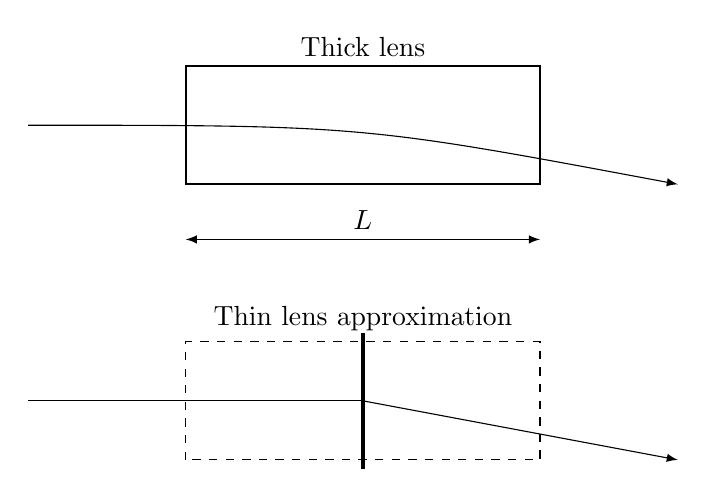
\begin{tikzpicture}
%    \draw[black,thin] (0.0,0.0) grid (16.0,9.0);

    % thick lens 
    \draw[thick] (6.0,4.5) rectangle (10.5,6.0);
    \draw[->] (4.0,5.25) .. controls (8.25,5.25) .. (12.25,4.5);
    \node [rotate=0]  at (8.25,6.25)    {Thick lens};


    %  thin lens
    \draw[dashed]      (6.0,1.0) rectangle (10.5,2.5);
    \draw[<->] (6.0,3.8) -- (10.5,3.8);
    \node [rotate=0]  at (8.25,4.05)    {$L$};

    \draw[thick] (8.24,0.9) rectangle (8.26,2.6);
    \draw (4.0,1.75)  -- (8.25,1.75);
    \draw[->] (8.25,1.75) -- (12.25,1.0);
   \node [rotate=0]  at (8.25,2.80)    {Thin lens approximation};


   
  \end{tikzpicture}
  \caption{Schematic illustration of the thin lens approximation. The transverse bending of a magnet of length $L$ is approximated by a point-like kick the particle receives only at the center of the magnet. Left and right of the magnet center the transverse particle momentum remains unchanged.}
  \label{pic:thinlens}
\end{figure}









The analytic treatment of the transfer matrices can be significantly simplified if the magnet length $L$ is small compared to $1/KL$. The magnetic bending can then be treated as a point-like transverse kick which is given to the particle at the center of the magnet. In the rest of the element length, the particle trajectory remains undisturbed, hence behaves like a drift space (see \figref{pic:thinlens}). Mathematically, this thin lens approximation~\cite{CERN-SL-95-12} corresponds to the limit
\begin{align}
  L \rightarrow 0 \quad \text{with} \quad K \, L = \text{const.} 
\end{align} 
The transfer matrix for a quadrupole magnet simplifies in the thin lens approximation to
\begin{align}
  \mathcal{M}_{Q,f/d} = \begin{pmatrix}  1 & L \\   KL & 1  \end{pmatrix} \, ,
\end{align}
which is equivalent to the transfer matrix of a thin optical lens with focal length $f=\frac{1}{KL}$.
%
\subsubsection{Periodic Solution and Betatron Motion}
An alternative to the solution of the homogeneous part of the equation of motion, given before in matrix form, is given by
%
\begin{align}
x(s) = \sqrt{\tilde{\epsilon}_x} \, \sqrt{\beta_x(s)} \, \cos \left( \psi_x(s) + \phi \right) \, , \label{eq:betatron_oscillation}
\end{align}
%
where $\tilde{\epsilon}$ and $\phi$ are mathematically the integration constants and represent the initial conditions of the particle. The function $\beta_x(s)$ is called the betatron function. The latter is related to the maximum amplitude the particle trajectory can take at the position $s$. 

\newpage
In circular accelerators the quantity $K(s)$ is periodic with the same period as the machine circumference $C$
\begin{align}
K(s) = K(s+C) .
\end{align}
The equation of motion (\ref{eq:hill1}) with periodic $K(s)$ is the Hill differential equation~\cite{wiedemann1999particle}. The solution of Hill's equation is identical to \eqref{eq:betatron_oscillation}, but the periodicity implies that also $\beta_x(s)$ is periodic in $s$ with period $C$
%
\begin{align}
  \beta_x (s) = \beta_x (s+C) \, .
\end{align}
The betatron function is purely defined by the magnetic lattice in the accelerator. The particles perform transverse quasi-harmonic oscillations in $x$, around the ideal trajectory. The local amplitude of these so-called betatron oscillations is defined by $\tilde{\epsilon}_x$, the betatron function $\beta_x(s)$ and the betatron phase $\psi_x(s)$, defined as
%
\begin{align}
  \psi_x(s) = \int_0^s \frac{\mathrm{d}s}{\beta_x(s)} \, .
\end{align}
%
The total number of betatron oscillations over one turn is called the machine tune
%
\begin{align}
  Q_x = \frac{1}{2 \pi} \int_0^C \frac{\mathrm{d}s}{\beta_x(s)} \, .
\end{align}
%
%
From \eqref{eq:betatron_oscillation} and its derivative, it can be deduced that $\tilde{\epsilon}_x$ is a constant of motion, mathematically the Courant-Snyder invariant, for the individual particle and can be expressed as
%
\begin{align}
\tilde{\epsilon}_x = \gamma_x(s) \, x^2(s) + 2 \, \alpha_x(s) \, x(s) \, x'(s) + \beta_x(s) \, x'^2 (s) \, . \label{eq:parameric_ellipse}
\end{align}
%
The quantities $\beta_x(s)$, $\alpha_x(s)$ and $\gamma_x(s)$ are the so-called Twiss parameters~\cite{wiedemann1999particle}. They are defined by the magnetic lattice in the machine which transforms the beam equivalently to a lattice of lenses in classical optics. The Twiss parameters are therefore also referred to as the optical functions, and the configuration of the magnetic lattice as the beam optics.

The derivative of the betatron function $\beta_x(s)$ defines the two remaining Twiss parameters as
\begin{align}
\alpha_x(s) = - \frac{1}{2} \beta_x'(s) \quad \quad \gamma_x(s) = \frac{1+\alpha_x(s)^2}{\beta_x(s)} \, .
\end{align}

%
\begin{figure}[b]  
    \centering
    \includegraphics[width=1\textwidth]{pictures/16021801.pdf}
    \caption{Individual particle trajectories in a periodic quadrupole lattice.}  
    \label{pic:16021801}
    %/home/phermes/Dropbox/PhD/pictures/160217_beam_enveloppe/enveloppe.pdf
\end{figure}

The evolution of an initial set $(\alpha_{x,0},\beta_{x,0},\gamma_{x,0})$ of Twiss parameters in the accelerator depends on the lattice elements and is, equivalent to the transformation of the particle coordinates in \eqref{eq:transfer_matrix}, described by their transfer matrices as follows
%
\begin{align}
  \beta_x(s) = C_x^2 \, \beta_{x,0} -2 \, S_x^2 \, C_x^2 \, \alpha_{x,0} + S_x^2 \, \gamma_{x,0} \, .
\end{align}
%
Furthermore, the expression in \eqref{eq:parameric_ellipse} is the parametric representation of an ellipse in $x,x'$ enclosing a phase space surface of $\pi \tilde{\epsilon}_x$. Shape and orientation of the phase space ellipse are changing as a function of the Twiss parameters. The surface in phase space that is enclosed by the ellipse remains unchanged if only conservative forces act on the beam particles (Liouville's theorem)~\cite{wiedemann1999particle}. Following \eqref{eq:betatron_oscillation}, the largest possible amplitude in $x$ and $x'$ the individual particle can reach yields (see \figref{pic:ell}):
%
\begin{align}
  x_\text{max} = \sqrt{\tilde{\epsilon}_x \, \beta_x(s)} \quad \text{and} \quad x_\text{max}' = \sqrt{\tilde{\epsilon}_x \, \gamma_x} \, .
\end{align}
%
The quantity $x_\text{max}$ is hence related to the peak amplitude of the betatron oscillation for a given $\beta$-function. If many particles compose the beam, the RMS value of the individual $\tilde{\epsilon}_x$ is referred to as the emittance, which is directly related to the RMS beam size $\sigma_x(s)$:
%
%
\begin{figure}[t]  
  \centering
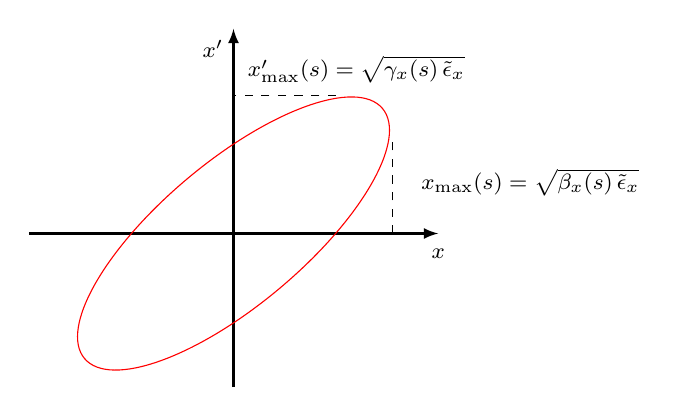
\begin{tikzpicture}[scale=1.3]
  \footnotesize
  % helper grid: comment for final drawing
  % \draw[help lines,step=.2] (0,0) grid (16.0,9.0);
  % \draw[help lines,line width=.6pt,step=1] (0,0) grid (16.0,9.0);
  % \foreach \x in {0,1,2,3,4,5,6,7,8,9,10,11,12,13,14,15,16}
  %      \node[anchor=north] at (\x,-0.1) {\x};
  % \foreach \y in {0,1,2,3,4,5,6,7,8,9}
  %     \node[anchor=east] at (-0.2,\y) {\y};

  % % text
  % \node [draw,rotate=90]  at (3.50,5.50)  {Injection};
  % % straight line and parabola
  % \draw [red,thick]          (0,0) -- (4,3);
  % \draw [black,thick,dashed] (0,0) parabola (4,4);
  % % bezier lines
  % \draw (6,0) .. controls (6,4) and (10,0) .. (10,4);
  % % circular shapes
  % \draw (5,5) circle (2cm);
  % \draw (7,2) ellipse (3cm and 1cm);
  % \draw (3,5) arc (0:75:3cm);
  % % filled rectangle



  % lower blms
%  \filldraw[fill=orange, draw=black] (9.2,3.8) rectangle (9.6,4.0);



  % % axes
  \draw[->,thick] (5,1.5) -- (5,5);
  \draw[->,thick] (3,3) -- (7,3);

  \draw[rotate around={40:(5,3)},red] (5,3) ellipse (1.9 and 0.7);

  % \draw[->,thick] (3.5,1) -- (3.5,4);
  % \draw[dashed] (3.5,2.0) circle (1.0);
  % \draw[red,thick,->] (3.5,3.0) arc (90:40:1.0);
  % \draw[red,thick,-] (3.5,3.0) arc (90:130:1.0);

  % \draw[->,thick] (3.5,2) -- (3.9,2.9);
  \draw[dashed] (6.55,3) -- (6.55,3.9);
  \draw[dashed] (6.0,4.35) -- (5.0,4.35);
  \node  at (7.9,3.5)  {$x_\text{max}(s) = \sqrt{ \beta_x(s) \, \tilde{\epsilon}_x}$};
  \node  at (6.2,4.6)  {$x_\text{max}'(s) = \sqrt{ \gamma_x(s) \, \tilde{\epsilon}_x}$};
  % \node  at (3.9,2.4)  {$\rho_0$};
  % \node  at (4.4,2.8)  {$S$};
  % \node  at (5.0,2.8)  {$z$};
  \node  at (7.0,2.8)  {$x$};
  \node  at (4.8,4.8)  {$x'$};
  % \node  at (4.3,3.4)  {$X$};

  % \draw[thick,->] (0,0) -- (0,4.5);

\end{tikzpicture}
  \caption{Phase space ellipse with $x_\text{max}$ and $x_\text{max}'$.}
  \label{pic:ell}
  \end{figure}
%
%
%
\begin{align}
  \sigma_x (s) = \sqrt{\epsilon_x \, \beta_x} \quad \text{with} \quad \epsilon_x = \langle \tilde{\epsilon_x} \rangle_{\text{rms}} \, .
\end{align}
%
The quantity $\sigma_x(s)$ defines an RMS beam envelope at the position $s$ which contains $1 \, \sigma_\text{rms}$ of the beam particles. In \figref{pic:16021801}, the betatron motion of particles with different initial conditions within $\epsilon_x$ is shown in a periodic lattice of quadrupoles and bending dipoles. It is clearly visible how the individual particle tracks are confined by $\sigma_x$.
%

The emittance is a measure for the beam quality and should be as small as possible. If the particle beam is accelerated, only the longitudinal momentum is increased. It can be shown that the ratio of transverse momentum to longitudinal momentum decreases $\frac{1}{\beta \, \gamma}$, which is referred to as adiabatic damping~\cite{wiedemann1999particle}. Consequently, the normalized horizontal emittance is defined as 
%
\begin{align}
  \epsilon_N = \epsilon_x \, \beta \gamma \, ,
\end{align}
and remains constant for all particle energies, assuming that, besides the acceleration, only conservative forces  act on the beam. The emittance is measured in units of $\mu$m rad.




\subsubsection{Solution of the inhomogeneous Equation of Motion}


The solution of the inhomogeneous equation of motion \eqref{eq:hill1} can be expressed as
%
\begin{align}
  x(s) = x_h(s) + x_i(s) \, , \label{eq:inhsol}
\end{align}
%
where $x_h(s)$ is the solution of the homogeneous equation shown in \eqref{eq:general_solution} and $x_i$ is one particular solution of the inhomogeneous equation, for example
%
\begin{align}
  x_i(s) = \bar{D}_x(s) \, \delta \, .
\end{align}
%
The dispersion function $\bar{D}_x(s)$ is a periodic function in $s$ with period length $C$, depending on the magnetic elements in the entire ring. It is defined as
%
\begin{align}
  \bar{D}_x (s) = - \frac{\beta_x(s)}{2 \, \sin (\pi \, Q_x)} \, \int_{s_0}^{s_0+C} \, h_x(\tilde{s}) \, \sqrt{\beta(\tilde{s})} \, \cos \left[ 2 \pi \, \left( \psi(\tilde{s}) - \psi(s_0) - \frac{Q_x}{s} \right) \right] \, \mathrm{d} \tilde{s} \, .
\end{align}

In order to be coherent with the definition in the simulation tools used, in the following the dispersion function will be expressed in terms of $D_x(s)$, defined as
%
\begin{align}
  D_x(s) = -\bar{D}_x(s) \, . \label{eq:dispoff}
\end{align}
%
As shown in \eqref{eq:inhsol}, the dispersion function relates the momentum offset of the particle to an additional transverse amplitude. The quantity $D_x (s) \, \delta$ hence gives the closed orbit around which  off-momentum particles perform betatron oscillations. For multi-isotopic beams, \eqref{eq:dispoff} still applies, but the relative momentum offset is replaced by $\delta_\text{eff}$.

It is often useful to also define the local dispersion function $\tilde{D}_x(s)$, which quantifies the dispersive offset an off-rigid particle acquires between two defined locations. This becomes important, when the rigidity of a particle changes at a given location and the particle trajectory should be followed from the location at which the rigidity offset was acquired.

Note that this mathematical description represents a linear approximation and higher order dispersive effects are not taken into account. For particles with large momentum offsets, a more accurate description is given by a fully symplectic transformation without truncation, which can be derived from the accelerator Hamiltonian (see \chapref{chap:hamiltonian}). 



\section{Longitudinal Particle Dynamics}

\input{pictures/cavity.tex}

The beams in the LHC are accelerated and longitudinally confined by means of radio frequency cavities (RF cavities)~\cite{wiedemann1999particle}. They consist of a periodic resonator structure (illustrated in \figref{pic:cavity}) and are operated with RF waves and provide a longitudinal electric field $V(t)$ of a defined frequency $\phi_\text{RF} = \omega_\text{RF} \, t$
%
\begin{align}
  V(t) = V_0 \, \sin (\phi_\text{RF} + \phi_s) \, ,
\end{align}
%
where $V_0$ is the peak amplitude of the electric field and $\phi_s = \omega_s \, t$ is the phase of the synchronous particle. The frequency of the RF cavity is adapted to the revolution frequency $f_\text{rev}$ of the synchronous particle, to provide the same accelerating voltage at every turn
%
\begin{align}
  f_\text{RF} = h \, f_\text{rev} \, ,
\end{align}
%
where $h$ is the harmonic number. Assuming that $q=q_0$, the energy $\Delta E$ transferred to a particle arriving at phase $\phi$ compared to the phase of the synchronous particle $\phi_s$ is given by~\cite{CAS2013}
%
\begin{align}
  \Delta E =  q_0 \, V_0 \, \left( \sin \phi - \sin \phi_s \right) \, .
\end{align}
%
The phase dependence of the energy transfer leads to a different energetic kick for particles arriving at different times than the synchronous particle. If $\phi_s$ is correctly chosen, particles with momentum $P$ smaller than the reference momentum $P_0$ (which arrive with time delay), receive a larger momentum transfer and those with $P>P_0$ receive a smaller momentum transfer than the synchronous particle. This is illustrated in the top plot of \figref{pic:16081703}. 

It can be shown~\cite{CAS2013} that the difference in phase $\Delta \phi = \phi - \phi_s$ with respect to the reference particle obeys the differential equation
%
\begin{align}
  \frac{ \mathrm{d}^2}{\mathrm{d} t^2 } \phi + \frac{\Omega_s^2}{\cos \phi_s} \, ( \sin \phi - \sin \phi_s ) = 0 \quad \text{with} \quad \Omega_s^2 = \frac{h \, \eta \, \omega_\text{rs} \, q_0 \, V_0 \, \cos \phi_s}{ C \, P_0} \, . \label{eq:syncmo}
\end{align}
Here, $h$ is the harmonic number, $\eta = \frac{\Delta \omega_\text{r}/\omega_\text{rs}}{\Delta P / P_0}$ is the slip factor which quantifies the change in revolution frequency implied by a change in momentum, $\omega_\text{rs}$ is the revolution frequency of the synchronous particle and $C$ is the circumference of the machine. 


\begin{figure}[t]
  \centering
  \begin{tikzpicture}
    \node[anchor=south west,inner sep=0] (image) at (0,0) {\includegraphics[width=0.6\linewidth]{pictures/16081703.png}};
    %\node [draw,rotate=90,x={(image.south east)},y={(image.north west)}]                   at (0.50,0.50)    {text0};
    %\node [draw,rotate=0 ,x={(image.south east)},y={(image.north west)}]                   at (0.22,0.96)    {text1};
    %\node [draw,rotate=0 ,x={(image.south east)},y={(image.north west)},anchor=west]       at (0.22,0.80)    {text2};
    %\draw[->,color=black,thick,x={(image.south east)},y={(image.north west)}]             (0.42,0.22) -- (0.37,0.23);
  \end{tikzpicture}
  \caption{Top panel: longitudinal electric field $V$ as a function of the particle phase $\phi$. Particles with $P<P_0$ which arrive later than the reference particle (1) receive a larger energy transfer. Accordingly, particles arriving before the reference particle (2) receive a smaller energetic kick. The particles perform an oscillation in the $\phi, \frac{\Delta P}{P_0}$-plane (bottom panel). The stable region in $\phi, \Delta P/P_0$ is defined by a separatrix. Figure courtesy of \cite{CAS2013}.}  
  \label{pic:16081703}
  %/home/phermes/Dropbox/PhD/thesis//home/phermes/Desktop/separartrix.png
  \end{figure}

For small phase deviations $\Delta \phi_s$, the expression in \eqref{eq:syncmo} can be simplified to~\cite{CAS2013}
%
\begin{align}
  \frac{ \mathrm{d}^2}{\mathrm{d} t^2 } \phi + \Omega_s^2 \,  \Delta \phi = 0 \, ,
\end{align}
which describes a harmonic oscillation (the so-called synchrotron oscillation) in $P$ and $\phi$, with frequency $\Omega_s$. Stability of the longitudinal motion implies that $\Omega_s^2>0$, which is the case when $\eta \, \cos \phi>0$, as illustrated in \figref{pic:16081703}.


Stable and unstable regions in the $\phi, \Delta P/P_0$ plane are separated by the so-called separatrix, which defines the largest amplitude in $\phi, \frac{\Delta P}{P_0}$ that is compatible with stable synchrotron oscillations. The region inside the separatrix is called RF bucket. 

By virtue of the periodicity of the electric field in the RF cavity, multiple buckets are available to store particles in the machine. The concrete number of buckets is determined by the harmonic number. Thus, the accelerating RF cavities imply a bunching of the particle beam. 





\chapter{The Large Hadron Collider}\label{thelhc}
%
\section*{Introduction}
%
\begin{figure}[b]
  \centering
  \includegraphics[width=0.6\textwidth]{pictures/14050501.png}
  \caption{LHC Beam Momentum vs. Stored Energy in comparison to other Particle Accelerators~\cite{Christiane:1260465}. In both means, the LHC is far beyond previous accelerators. The maximum stored energy in the LHC will be 362\,MJ. } \label{pic:14050501} 
\end{figure}
%
The Large Hadron Collider (LHC) is the world's largest and most particle accelerator, designed to store and accelerate proton and \lead beams at unprecedented energies of 7$\,Z\,$TeV. The LHC is a synchrotron of 26.7\,km length, installed in the underground tunnel of the former LEP\footnote{Large Electron Positron collider} accelerator at the CERN\footnote{Centre Europ\'{e}en pour la Recherche Nucl\'{e}aire} research center in proximity to Geneva, Switzerland. Besides the Relativistic Heavy-Ion Collider (RHIC) at the Brookhaven National Laboratory in Long Island (USA), it is one of the two heavy-ion colliders operating worldwide and the third heavy-ion collider ever built~\cite{Fischer2014}. In the first operational period (LHC run 1), the LHC reached energies up to 4$\,Z\,$TeV and collected an integrated luminosity of 29.2\,fb$^{-1}$~\cite{lamont_moyab101} with proton beams and xx.x\,fb$^{-1}$ with \lead beams. With the collected data, the discovery of the long sought Higgs Boson could be announced in July 2012~\cite{}. After a phase of machine and detector upgrades from 2013 to 2015, the LHC re-started and accelerated proton beams to the unprecedented energy of $6.5\,$TeV.
%
%
%
%Breaking many barriers in terms of beam intensity and energy, the topic of collimation was never as important as for the LHC.  
%
%
%\newpage

\section{The LHC Accelerator Complex}

  \begin{figure}[t]
  \centering
  \includegraphics[width=1.0\textwidth]{pictures/14052201.png}
  \caption{ The CERN Accelerator Complex }  
  \label{pic:14052201}
  \end{figure}

High energy accelerators like the LHC can not be operated independently, but are installed at the end of a complex chain of injectors which pre-accelerate and shape the beam for the requirements of the end using machine. The CERN accelerator complex is schematially illustrated in Fig.~\ref{pic:14052201}. The generation of proton beam starts at an ion source 

% PH: 140516
Heavy-ion beams originate from the ion source which is connected upstream of the linear accelerator LINAC3. The ions are generated from a block of isotopically pure $Pb^{208}$ by means of microwave heating~\cite{}. The source delivers ions at a momentum\footnote{For clarity, in this chapter the momementum is given in natural units. All given momenta shall correspond to the correct unit of eV$/c$. Furthermore, the energies for the non fully stripped ions are given in terms of momentum per nucleon, while for the fully stripped ions, the general convention of using the momentum per charge is followed.} of 2.5\,keV/$u$, which are sent to a spectrometer in order to extract the desired Pb$^{+27}$ charge state. After the filtering, a multi-stage RF system accelerates the selected ion species to a momentum of $4.2\,$MeV/$u$. The following stripper foil removes more electrons, such that an ion beam of Pb$^{+53}$ is extracted from LINAC3 and transferred to the circular accelerator LEIR (Low Energy Ion Ring). In the latter, the ion beams are cooled, e.g. the transverse emittance (see \chapref{}) is reduced by an adiabatic process using electron scattering. In parallel, the beam is accelerated to a momentum of 72$\,$keV$/u$ at which it is extracted and transferred into the Proton Synchrotron (PS). At this machine, the ions are accelerated to a momentum of 5.9$\,$GeV$/u$ and sent to the Super Proton Synchroton (SPS). 

A final stripper foil installed at the PS-SPS transfer line removes the remaining electrons from the ions, such that a beam of \lead is injected into the SPS. The SPS provides the acceleration to the energy of $450\,Z\,$GeV at which the beams are injected into the LHC.


\section{LHC Layout}
\subsection{Global Layout}

\figref{pic:15032201} shows the LHC layout with its eight straigt insertion regions (IR), four of which host the main experiments (IR1, IR2, IR5 and IR8) and four providing operational functionalities. The straight sections are seperated by eight arc regions, in which the particle beams are transported from IR to IR by means of a total of 1232 superconducting dipole magnets and 392 superconducting quadrupole magnets in a so-called FODO lattice. 



  \begin{figure}[t]
  \centering
  \includegraphics[width=0.7\textwidth]{pictures/15092509.pdf}
  \caption{The layout of the LHC. Based upon \cite{Bruning2012705,CERN-2004-003-V1}. }  
  \label{pic:15032201}
  %/home/phermes/Dropbox/codes/latex/150305_eps2pgf/test.pdf
  \end{figure}


\subsection{Insertion Region Layout}




\section{Beam Parameters}

%%%%%\multicolumn{1}{l|}{$^{208}_{82}$Pb}

The LHC Beam Parameters for protons and lead ions are summarized in \tabref{tab:14052101}. In heavy ion operation, the design luminosity is significantly smaller than for proton operation, which can be traced back to the lower number of bunches and the smaller number of bunches per beam. 

%\begin{table}[htb

% \begin{table}[htbp]
% \caption{Comparison of LHC beam parameters in proton and lead mode~\citedr. }
% \begin{center}
% \begin{tabular}{lccc}
% \toprule
% \midrule
%  & & Proton & $^{208}$Pb$^{+82}$ \\ \midrule
% Total energy &[GeV]\phantom{abc} & 7000 & 574000 \\ \midrule
% Energy per nucleon &[GeV]\phantom{abc} & 7000 & 2759 \\ \midrule
% Lorentz factor $\gamma$ &\phantom{abc} & 7461 & 2963.5 \\ \midrule
% Normalized tr. emittance  &[$\mu$m rad]\phantom{abc} & 7461 & 2963.5 \\ \midrule
% Stored Energy per beam  &[MJ]\phantom{abc} & 362 & 3.81 \\ \midrule
% Particles per bunch  &\phantom{abc} & $1.15 \cdot 10^{11}$ & $7 \cdot 10^{7}$  \\ \midrule
% Number of bunches  &\phantom{abc} & 2808 & 592  \\ \midrule
% Design luminosity  &[cm$^{-2}\,$s$^{-1}$]\phantom{abc} & $1\cdot 10^{34}$ & $5.4\cdot 10^{25}$  \\ \midrule
% \bottomrule
% \end{tabular}
% \end{center}
% \label{tab:14052101}
% \end{table}

\section{The LHC as a Nucleus-Nucleus Collider}

The LHC is one of the two operating heavy-ion colliders worldwide. Other than the LHC only the Relativistic Heavy-Ion Collider (RHIC) at the Brookhaven National Laboratory in Long Island is presently in operation, but provides energies far below the LHC design collision energy. The beam parameters for the LHC in heavy-ion operation are summarized in \tabref{tab:lhc_parameters}. Especially in terms intensity, emittance and luminosity, the LHC has outreached the design values. The number of 

\begin{tiny}
\begin{table*}[t]
\centering
\caption{Comparison of the LHC design beam parameters for heavy-ion beams and proton beams in comparison to the parameters typically achieved in the LHC heavy-ion runs.~\cite{CERN-2004-003-V1,pPbref01,jowett-RLIUP13,PbPbref01,Jowett:1492972}. The parameters given for p-Pb operation refer to the \lead beam.}
\label{tab:lhc_parameters}
\begin{tabular}{cc|cc|cccc}

\multicolumn{2}{c|}{} &  \multicolumn{2}{c|}{Nominal} & \multicolumn{4}{c}{Achieved in the LHC} \\ \toprule

\multicolumn{2}{c|}{Year}     &  &  & 2010 & 2011 & 2013 & 2015 \\% \midrule
\multicolumn{2}{c|}{Species}  & p-p & Pb-Pb & Pb-Pb & \multicolumn{1}{c}{Pb-Pb} & p-Pb & \multicolumn{1}{c}{Pb-Pb} \\ \midrule


$E$ & {[}TeV{]} & 7 & 7$\,Z$ & 3.5$\,Z$ & 3.5$\, Z$ & 4.0$\, Z$ & 6.37$\,Z$\\

$\gamma$ & & 7460.5 & 2963.5 & 1481.8 & 1481.8 & 1693.4 & 2696.8\\

$n_b$ & & 2808 & 592 & 137 & 358 & 338 & 111\\

$n_p$ &{[}$10^8${]} & 1.15$\times 10^{3}$ & 0.7 & 1.12 & $1.20 \pm 0.25$ & $1.40\pm0.27$ & $1.11$\\

$\epsilon_N$ & {[}$\mu$m$\,$rad{]} & 3.75 & 1.5 & 2.0 & $1.7\pm0.2$ & - & 1.11 \\

$E_s$ &{[}MJ{]} & 362 & 3.81 & 0.71 & 1.98 & 2.18 & 1.11\\

$\mathcal{L}_\text{peak}$ &[$10^{27}\,$cm$^{-2}\,$s$^{-1}$] & $1.0\times 10^7$ & \begin{tabular}[c]{@{}l@{}}1 (Pb-Pb)\\ 115(p-Pb)\end{tabular} & 0.03 & 0.5 & 110 & 111\\ 

\bottomrule
\end{tabular}
\end{table*}
\end{tiny}
%\chapter{Collimation at the LHC}\label{chap:3}
%
\section*{Introduction}
%
At design energy and beam intensity, the LHC stores proton beams with a combined energy of $2 \times $362$\,$MJ~\cite{CERN-2004-003-V1}, corresponding to the amount of energy required to melt 600$\,$kg of copper. Besides the highly destructive potential of such energetic beams, which could cause serious damage at LHC components, already tiny amounts of this energy suffice to quench the superconducting LHC magnets~\cite{}. Such quenches are undesired because they interrupt the operation of the machine and reduce the time available to collect integrated luminosity for the experiments and therefore the statistics for rare events occuring at the particle collisions. 

Many processes continuously scatter beam particles to large transverse amplitudes or cause them to lose fractions of their momentum. One example for these processes is intra-beam scattering (IBS). Particles which have been scattered to such large amplitudes compose a beam halo which continues moving inside the machine. If no countermeasures are taken, these halo particles are scattered further outside until they have reached a large enough amplitude to be absorbed at the global machine aperture bottleneck. The processes which continuously re-populate the beam halo can not be avoided such that beam losses during machine operation become unpreventable. 

The ensemble of particles at betatronic amplitudes far from those of the beam core are referred to as the beam halo. In order to avoid uncontrolled losses of such halo particles, they are removed from the beam by intercepting them with a set of dedicated solid devices, the LHC collimation system. 

In this chapter, the design, functionality and performance of the LHC collimation system are discussed for both, proton and heavy-ion beams.



%
\section{The LHC Collimation System}
\subsection{Concept}
  \begin{figure}[t]
  \centering
  \includegraphics[width=1.0\textwidth]{pictures/15071301.pdf}
  \caption{Schematics of the LHC multi stage collimation system. Particles at large betatronic amplitudes are intercepted by the primary collimators (TCP) from which they should be scattered to even larger amplitudes to be captured by the secondary collimators (TCS), which are equipped with dedicated shower absorbers (TCLA). Particles escaping from the TCS constitute a tertiary beam halo which would be absorbed in the global aperture bottleneck, which are the superconducting triplet magnets in the experimental insertions. Therefore, the latter are protected with the tertiary collimators (TCT). Particles which have lost energy but have not been scattered enough in the TCP can still bypass the TCS and are most likely absorbed in the dipole magnets of the LHC arcs, where the dispersion rises.}  
  \label{pic:15071001}
  %/home/phermes/Dropbox/PhD/pictures/collimationsystem_drawing_thesis/drawing2.pdf
  \end{figure}

The aim of the system is the interception and controlled absorption of the transverse beam halo which is continuously re-populated during operation~\cite{}. In other accelerators, such halo particles can be intercepted and absorbed by means of collimators with two movable jaws that are brought closely to the beam center~\cite{}. Contrary to such low-energy machines, the highly energetic and destructive LHC beam halo can not be removed from the beam by means of a single collimation unit. With the high particle momenta and the large stored beam energies, no known material possesses a large enough absorption cross section and radiation hardness to immediately stop halo particles circulating in the LHC. Therefore, the LHC is equipped with a three-stage collimation system which is schematically illustrated for the example of the betatron cleaning insertion IR7 in \figref{pic:15071001}.

The primary beam halo of particles at large betatronic amplitudes is intercepted with the primary collimator (abb. Target   Collimator  Primary, TCP). This collimator type is the only collimator which should be exposed to the main beam. In order to provide enough radiation hardness, the collimator jaws are composed of a dedicated carbon-fibre composite (CFC). The collimation system relies upon the scattering of the halo particles at their passage through the CFC to even larger betatronic amplitudes. If a halo particle receives a sufficiently large transverse kick, it is intercepted by the secondary collimators (abb. Target Collimator Secondary, TCS). 

The TCS collimators are retracted with respect to the TCP, thus it should be only exposed to the secondary beam halo which carries a significantly lower amount of energy. Compared to the TCP collimators of 0.6$\,$m length, the TCS collimators are significantly longer being 1$\,$m long. Downstream of the TCS collimators, the secondary shower absorbers shall provide protection from particle showers arising from the interaction with the TCS.

Scattered particles can still leak out of the TCS collimators and continue moving inside the machine (the so-called tertiary beam halo). In the LHC high luminosity mode with squeezed beams in the experimental insersions, these particles are most likely absorbed in the triplet magnets where the betatronic functions are extreme. In order to avoid beam losses in the triplet magnets, they are protected by the tertiary collimators (abb. Target Collimator Tertiary, TCT). This collimator type consists of copper to provide a high absorption cross section. The three described stages compose the three stage collimation system of the LHC.

\begin{figure}
\centering
\resizebox{1.0\textwidth}{!}{\input{pictures/14121239.pgf}}
\resizebox{1.0\textwidth}{!}{\input{pictures/14121503.pgf}}
%\resizebox{1.0\textwidth}{!}{\input{pictures/14121222.pgf}}
\caption{Optical functions in the two LHC collimation insertions.}
\label{pic:14121222}
\end{figure}

The functionality of the momentum cleaning insertion in IR3 is the same as for IR7, with the difference that the optics in IR7 is matched for large betatronic functions at the TCP, while in IR3 it is matched for a larger dispersion function (see \figref{pic:14121222} for a comparison). In consequence, the TCP in IR3 intercepts off-momentum particles rather than particles at large betatronic amplitudes. 

Besides the presented collimators of the three-stage collimation system, functional collimators are installed for other purposes than halo-cleaning. The TDI collimators installed in the two injection insertions IR2 and IR8 protect the LHC hardware from beam loss which could occur due to injection failures. They are composed of graphite in a different alloy than the CFC used for the TCP and TCT collimators. In order to protect a larger area in phase space, the TCLI collimators are installed downstream of the TDI. In case of a dumping failure, multiple components of the LHC could be seriously damaged, in particular the dumping system, magnets downstream of IP6 or even the detector components in the experimental insertions. Therefore, IR6 is equipped with the single-jaw dump protection collimator TCDQ and the double-jaw TCSG collimator (the same collimator type as it is used for the secondary collimators in IR3 and IR7). The jaw of the prior is composed of graphite and is the longest collimator used in the LHC having a length of 6$\,$m. 

An overview of the different collimator types is given in \tabref{tab:collimator_types}. In the design phase of the machine, a progressive upgrade of the LHC collimation system was foreseen to increase the performance of the protection with increasing luminosity and energy~\citedr. 


 \subsection{Collimator Settings}


\begin{table}[htbp]
\caption{LHC collimator settings applied in the LHC heavy ion runs compared to the design settings. }
\begin{center}
\begin{tabular}{lcccccc}
\toprule
\midrule
 \multicolumn{2}{c}{Collimator} & \multicolumn{4}{c}{Half gap ($\sigma$)} \\
Type & Region & 2010 & 2011 & 2013 & 2015 & Design \\ \midrule
TCP  & IR7 & 5.7  & 5.7  & 4.3  & 9.9 & 6.0  \\
TCS  & IR7 & 8.5  & 8.5  & 6.3  & 9.9 & 7.0  \\
TCLA & IR7 & 17.7 & 17.7 & 8.3  & 9.9 & 10.0 \\ \midrule
TCP  & IR3 & 12.0 & 12.0 & 12.0 & 9.9 & 15.0 \\
TCS  & IR3 & 15.6 & 15.6 & 15.6 & 9.9 & 18.0 \\
TCLA & IR3 & 17.6 & 17.6 & 17.6 & 9.9 & 20.0 \\ \midrule
TCT  & IR1/IR2/IR5/IR8    & 15.0 & 11.8 &  9.0 & 9.9 & 8.3  \\ \midrule 
 \multicolumn{2}{c}{Energy [TeV]} & 3.5 & 3.5 & 4.0 & 6.5 & 7.0 \\
\bottomrule
\end{tabular}
\end{center}
\label{tab:14070901}
\end{table}

The multi-stage collimation system relies upon the scattering of the halo-particles 

The functionality of the LHC betatron cleaning system is schematically illustrated in \figref{pic:14052202}. In the collimation regions IR3 and IR7, primary collimators (TCPs) are set to a collimator opening of $N_1$ (transverse distance from beam centre expressed in terms of $\sigma$) to intercept the trajectories of particles at large amplitudes. These particles interact with the collimator material, such that they are either scattered back into the beam or to a larger amplitude~\citedr.\

Depending on the angular kick, the latter can then intercept the secondary collimators (TCS) of opening $N_2$, which is slightly retracted with respect to the TCPs ($N_2>N_1$). This is provided, if the angular kick $\Delta x'$ fulfills the condition~\cite{jeanneret1998optics}

\begin{align}
\Delta x' > \sqrt{\frac{(N_1^2 - N_2^2) \, \epsilon_N }{ \gamma \, \beta_x } } \,,
\end{align}
where $\epsilon_N$ is the transverse normalized emittance, $\beta_x$ is the horizontal optical $\beta$-function at the primary collimator and $\gamma$ is the Lorentz factor.


\section{Measurement of Losses during LHC Operation}

The LHC is equipped with more than 4500 ionization chambers, the beam loss monitors (BLM)~\cite{BLMref1,BLMref02}, installed at the outer side of superconduction magnets, collimators and other locations which keep track of the particle losses at the particular locations. The ionization chambers measure secondary particle showers arising from the interaction of the ultra-relativistic particles interacting with the collimator material or with the beam pipe and surrounding components if they are lost. The BLM data is continuously monitored by the LHC interlock system which triggers a beam dump if a certain loss threshold is exceeded~\cite{guaglio2005reliability}. This is done to protect the machine from beam damage e.g. in the case of sudden instabilities or changes in the beam configuration inducing too much losses. Also losses of collisional debris can be monitored with this system. The so-obtained data is used to show the longitudinal distribution of losses as a so-called physics loss map.

Besides the monitoring of the losses in operation, the BLM system can be used for a dedicated evaluation of the cleaning efficiency of the collimation system if the beams are excited to large transverse amplitudes or purposely momentum shifted by the RF system. This kind of measurement is described in the following as a qualification loss map.

\subsection{The LHC Beam Loss Monitors}
\begin{figure}[t]
  \centering
   \def\svgwidth{1.0\linewidth}
   \input{pictures/hybrid_pictures/14062001.pdf_tex}
  \caption{Illustrated positioning of BLMs at a superconducting LHC magnet~\cite{dehning2002lhc}.}
\label{pic:14061701}
\end{figure}
%
The BLMs used at the LHC are ionization gas detectors of cylindrical shape, which are installed outside the beam pipe. They measure the particle showers which are produced by a particle hitting the LHC beam pipe.
Inherently, the BLMs do not provide full azimutal or longitudinal coverage, such that the BLM response for the same amount of lost particles may vary between two different locations. Thus, the comparability of experimental measurements of the distribution of loss positions in the machine (lossmaps) with simulation data is therefore limited. Also, the translation of BLM signals into magnet heating and therefore the quench limit in terms of BLM signal is not trivial. Dedicated monte carlo simulations are necessary, in order to estimate the heating at a specific magnet due to a specific configuration of initial particle hits, under respect of the individual magnet geometry. However, the measurements give a very good idea of frequent loss positions and approximately the expectable loss intensity. 


\subsection{Physics Loss Maps}

During operation of the LHC, the losses in the machine are continuously monitored. The losses observed in this case arise from many different effects, the most important ones are summarized in the following:
%
\paragraph{Collimation losses} Different physical processes continuously re-populate the beam halo or lead to an energy loss of the involved particles. These particles should be intercepted by the LHC collimation system. The losses are registered by the BLMs installed at the collimators. Furthermore losses at the magnets arise from particles escaping from the collimation system. 
%
\paragraph{Losses from temporary instabilities} Furthermore, changes of magnet strengths, for example occuring during the ramp or squeeze, may lead to temporary instabilities causing losses that can be monitored by means of the BLM system. 
%
\paragraph{Physics debris} Debris from the experiments can involve [...] for protons. For the case of heavy-ions important debris arises from the bound free pair production (BFPP) process from the interaction of two \lead ions closely encountering each other at the interaction point. During the encounter of the two particles, an electron-positron pair is produced by the exchanged photon. The electron is then captured by the electron shell of one of the two involved nuclei:
\begin{align}
^{208}\text{Pb}^{82+} + ^{208}\text{Pb}^{82+} \rightarrow ^{208}\text{Pb}^{82+} + ^{208}\text{Pb}^{81+} + e^+ \, .
\end{align}
Compared to the fully stripped nucleus, the $^{208}\text{Pb}^{81+}$ ion possesses a different mass to charge ratio and is thus subject to dispersion. The ion is lost at the DS at the end of the IR. Owing to the large cross section of the process, the BFPP loss is dominant in the physics loss map during heavy-ion operation.

Examples for physics loss maps are shown for the case of proton and heavy-ion beams in \figref{fig:physics_loss_maps1}. In the measured loss map the contributions from the two beams can not be distinguished. Also, it is in general not trivial to de-convolute the contributions of the different processes described above. 
%
\subsection{Qualification Loss Maps}


In order to selectively study the cleaning efficiency of the LHC collimation system the collimation losses must dominate in the loss maps.


[] AC Dipole for beam excitation
[] Resonance crossing techniques



\section{Collimation of Heavy-Ion Beams at the LHC}

At their passage through matter, heavy ions interact differently than protons. Instead of being mainly scattered to larger transverse amplitudes as it is the case for protons, ions are less subject to scattering but have large cross-sections for the fragmentation into other isotopes.  In this section the interaction of ions with matter is discussed and the consequences on the collimation efficiency are outlined. The collimation efficiency measured at the LHC is compared for heavy-ion beams and proton beams.


\subsection{Heavy-Ion Qualification Loss Maps}

\begin{figure}[b]
  \begin{center}
\begin{minipage}[t]{0.49\textwidth}
\includegraphics[width=1\textwidth]{pictures/15091803.pdf}
\end{minipage}
\begin{minipage}[t]{0.49\textwidth}
\includegraphics[width=1\textwidth]{pictures/15091802.pdf}
\end{minipage}
%\includegraphics[width=0.49\textwidth]{pictures/15091801.pdf}
%\includegraphics[width=0.49\textwidth]{pictures/15091802.pdf}
\caption{Qualification loss maps with proton and \lead beams at $3.5\,Z\,$TeV with identical collimator settings and optics, except in IR2. The proton loss map is taken from \cite{Bruce2014a}. Both measurements were taken during the 2011 proton and heavy-ion operation. The vertical dashed lines mark the LHC octants. The upper plots show the full LHC ring, the bottom plots a zoom to IR7.}
\label{fig:meas_lm_comparison}
  \end{center}
\end{figure}


In Fig.~\ref{fig:meas_lm_comparison} qualification loss maps are compared from measurements taken in 2011 with heavy-ion beams and proton beams at energies of $3.5\,Z\,$TeV with identical optical und collimator settings, except in IR2. In the latter, heavy-ion beams were squeezed to \mbox{$\beta^*=0.8\,$m} instead of the $\beta^*=10\,$m applied for protons. The applied collimator settings are summarized in Tab.~\ref{tab:14070901}. As usual, all BLM signals are normalized to the highest signal, typically seen at the TCP or just downstream. 

\textit{The heavy-ion loss distribution is dominated by losses in the betatron collimators of IR7, followed by the momentum collimators in IR3. Downstream of the betatron collimation region, two loss clusters in the dispersion suppressor region were measured at amplitudes of $\eta_\text{max} = 10^{-2}$ (two orders of magnitude larger than the DS loss clusters for protons). Four loss peaks at $\eta_\text{max} = 10^{-4} - 10^{-2}$ are present downstream of the dispersion suppressor in the arc magnets between IR7 and IR8. The losses at the TCT in IR8 are smaller with heavy-ion beams than for proton beams. Two loss peaks in the arc region between IR8 and IR1 are visible in both loss maps, but is larger by 2-3 orders of magnitude for the heavy-ion beam. The TCT losses in IR1 are followed by a large loss peak in the arc region between IR1 and IR2, with $\eta_\text{max}=10^{-3}$. While IR2 is free of losses beyond the noise level in the proton loss map, four major loss peaks, one being at the TCT, are visible in octant 2 with the heavy-ion beams. The difference loss patterns in this region can be explained from the different optical configuration used in the two measurements. The loss rate in IR3 is larger by 2 orders of magnitude for the heavy-ion case, indicating the large amount of effectively off-momentum ions which is present in the machine. The losses at the IR5 TCT and the dump protection devices in IR6 are higher with proton beams than with heavy-ion beams.}

In the IR7 DS, the collimation efficiency for heavy-ion beams is worse by two orders of magnitude with respect to proton beams. 



\begin{table}[htbp]
\caption{Physics processed of protons and lead ions in the collimator material, with characteristic quantities~\cite{braun2004collimation}.}
\begin{center}
\begin{tabular}{ l c c }
\toprule
Physics Process & Proton & \lead \\ \midrule
$\frac{dE}{E\,\mathrm{d}x}$ due to ionization & -0.0088\%/m & -0.73\%/m \\ 
Multiple Scattering (projectred r.m.s. angle) & 4.72$\,\mu$rad/$\sqrt{m}$ & 4.72$\,\mu$rad/$\sqrt{m}$ \\ 
Nuclear Interaction length ($\approx$ fragmentation length) & 38.1$\,$cm & 2.5$\,$cm \\ 
Electromagnetic dissociation length & - & 19$\,$cm \\ \bottomrule
\end{tabular}
\end{center}
\label{}
\end{table}

\subsection{Ion-Matter Interaction} \label{chap:ionmatterinteraction}

Ultrarelativistic ions interact (collide) with the atoms of the traversed material in different manners. Such collisions do not require a physical overlap of the involving particles, but it is sufficient if the impact parameter $b$ (the smallest distance between the projectile and the target) is small enough such that a strong or electromagnetic interaction can take place. 

\subsubsection{Energy Loss from Ionization}

  \begin{figure}[b]
  \centering
  \includegraphics[width=0.85\textwidth]{pictures/15091401.png}
  \caption{}  
  \label{pic:15091401}
  %/home/phermes/Desktop/lec1.png
  \end{figure}

Particles at the passage through matter can interact inelastically with the electrons of the constituing atoms. At such encounters, the target atoms are ionized and the liberated electron receives a fraction of the projectile's kinetic energy. This energy loss is described by the Bethe-Bloch formula:
\begin{align}
- \left\langle\frac{dE}{dx}\right\rangle = \frac{4 \pi}{m_e c^2} \cdot \frac{nz^2}{\beta^2} \cdot \left(\frac{e^2}{4\pi\varepsilon_0}\right)^2 \cdot \left[\ln \left(\frac{2m_e c^2 \beta^2}{I \cdot (1-\beta^2)}\right) - \beta^2\right]
\end{align} \, .
The average energy loss depends on the projectile mass and velocity and on the atomic density of the target. The energy loss is shown in function of $\beta \gamma$ and the particle type in \figref{pic:15091401}.

\subsubsection{Electromagnetic Dissociation}
Electromagnetic dissociation occurs at ultraperipherical collisions of the involved nuclei ($b>R_1 + R_2$). The Lorentz contracted electric fields lead to the exchange of a large number of virtual photons that can induce the nuclear excitation of one or both of the involved nuclei. The excited nuclei decay under the emission of one or more nucleons, where the emission of neutrons has the largest cross section for heavy nuclei such as \lead. An important example for the electromagnetic dissociation of lead is the production of $^{207}$Pb$^{82+}$ in the carbon material of the primary collimators 
\begin{align}
^{208}\text{Pb}^{82+} &+ ^{12}\text{C} \rightarrow ^{207}\text{Pb}^{82+}  + ^{12}\text{C} + n \, .
\end{align}
The resulting heavy ion can be subject to a sub-sequent EMD resulting in $^{206}$Pb$^{82+}$, a main contributor to the ion losses in the aperture of the LHC arcs, as discussed in \chapref{chap:isocontributions}.

\subsubsection{Nuclear Fragmentation}
Nuclear encounters with impact parameters smaller or equal than the sum of the radii of the involved nuclei can lead to interactions by means of the strong force. One or both of the overlapping nuclei desintegrate typically into many different nuclear fragments. The particular composition of isotopes generated by such an interaction is different for every interaction. 

\subsubsection{Multiple Coulomb Scattering}

Coulomb scattering occurs if the projectile is deviated from its trajectory while interacting with the coulomb field of the atoms in the collimator material.This elastic scattering can occur many times throughout the passage through the collimator materials, thus the many small scattering angles can superimpose to a larger final angle at exit of the material. The RMS angle due to multiple Coulomb scattering is well-described by the Moliere formula~\cite{Beringer:1900zz}
\begin{align}
\theta_0 = \frac{13.6\,\text{MeV}}{\beta \, c \, p} \, Z \, \sqrt{\frac{\Delta s}{X_0}} \, \left[ 1 + 0.038 \, \ln \left( \frac{\Delta s}{X_0} \right) \right] \, ,
\end{align}
where $\beta\,c = v$ and $p$ are particle speed and momentum, $\Delta s$ is the distance the particle traversed inside the material, $Z$ is the charge of the beam particle and $X_0$ is the characteristic scattering length (see \chapref{xxx}). The latter is depending on the material and is either accessible via tabulated data or by means of the approximated formula in function of the charge $Z_m$ and nucleon number $A_m$ of the atoms constituing the material:
\begin{align}
X_0 = \frac{716.4 \, A_m}{Z_m (Z_m+1) \, \ln (287/\sqrt{Z_m})} \, .
\end{align}


\subsection{Fragmentation and Scattering at the Primary Collimators}

 \begin{figure}[b]
 \begin{minipage}[t]{0.5\textwidth}
 \includegraphics[width=1\textwidth]{pictures/15091301.pdf}
 \end{minipage}
 \begin{minipage}[t]{0.5\textwidth}
 \includegraphics[width=1\textwidth]{pictures/15091003.pdf}
 \end{minipage}
 \caption{Comparison of the distribution $P_\text{eff}$ and the scattering angle of particles leaking out the TCP carbon material between a proton beam (top) and a heavy-ion beam (bottom). The simulation was carried out using FLUKA at an energy 3.5$\,Z\,$TeV with the beam impacting perpendicularly at a carbon target of thickness $10.3\,$cm. The thickness corresponds to the interaction length in the TCP material with an impact parameter of $b=3\,\mu$m (see Sec.~\ref{chap:stier_description}).} %The black lines indicate $\pm \Delta \theta_\text{min}$ as shown in Eq.~(\ref{minkick}). Ions with $\Delta \theta$ between the two lines are not captured by the secondary collimators. }
 \label{fig:15022301}
 \end{figure}




The momentum per nucleon $p=P/A$ and the transverse angle of the fragment trajectories $\theta$ therefore acquire offsets of $\Delta p,\Delta \theta$ with respect to the heavy-ion which initially impacted the collimator material.



\begin{figure}[b]
  \begin{center}
\includegraphics[width=0.65\textwidth]{pictures/15091004.pdf}
\caption{Energy fraction of particles leaking out of the primary collimator which are uncaptured by the secondary collimators. Simulation carried out by FLUKA for an initial proton beam (blue) and \lead beam (black). Out-scattered protons are mostly concentrated at the reference momentum $P_E=3500\,\text{GeV}/c$. On the contrary, many ion fragments are effectively off-momentum and therefore likely to be absorbed in the aperture at a dispersive maximum. The dashed lines show the integral of the fragment energy starting at 1000$\,$GeV/$c$. Only 0.5\% of the escaping proton energy is carried by particles with rigidity offsets larger than 1\%, while for ions the corresponding value is 84.2\%. }
\label{fig:15062510.pdf}
  \end{center}
\end{figure}
 



To visualize the difference between fragmentation of  \lead ions and scattering of protons in the material of the primary collimators, two dedicated simulations were carried out with FLUKA~\cite{bohlen2014fluka,ferrari2005fluka}. In both cases, a particle beam with an energy of $3.5\,Z\,$TeV is simulated to perpendicularly hit a carbon target of 10.3$\,$cm thickness. This corresponds to the interaction length of the heavy-ions in the primary collimator with an impact parameter of $b=3\,\mu$m (see Sec.~\ref{chap:stier_description}). The resulting distribution in $P_E$ and the scattering angle $\theta$ of all out-coming particles is presented for both simulations in Fig.~\ref{fig:15022301}. The two horizontal lines respresent the minimum anglular kick required such that a particle intercepts the secondary collimator, as calculated using Eq.~(\ref{minkick}). We consider the collimator openings shown in Tab.~\ref{tab:collimator_gaps} and a normalized emittance of $\epsilon_N=3.5\,\mu$m rad. All ions in between these lines are not captured by the secondary collimators. The proton spectrum shows a sharp cut at $P/q=3.5\,$TeV/$c$, while the heavy-ion fragments can have larger effective momenta than the impacting ion, if $\chi>1$. 

% Fig.~\ref{fig:15022301} shows the distribution of momentum per charge vs. the scattering angle of atomic nuclei produced by the interaction of an initial proton beam compared to an initial \lead beam at $3.5\,Z\,$TeV with the solid graphite material of the horizontal LHC IR7 TCP as simulated with FLUKA. In the simulated case, the incoming beams hit the collimator material at an angle $\theta<0$ with an impact parameter (the transverse distance of the impacting particle beam from the collimator edge) of $b=3\,\mu$m as shown in Fig.~\ref{fig:15021801.pdf}. Therefore, particles with positive scattering angles are suppressed in the spectrum, due to their larger interaction length in the material.


On the basis of this simulation, Fig.~\ref{fig:15062510.pdf} shows the distribution of particles which have not received an angular kick large enough to be captured by the secondary collimators, in function of the momentum per charge unit. For the proton case, the energetic fraction carried by particles with $P_E \ll 3500\,\text{GeV}/c$ takes values between $10^{-5}$ and $4 \times 10^{-5}$ and the distribution shows only a sharp peak at the reference energy. We conclude that in this case, only small amounts of the uncaptured protons have significant momentum offsets and are likely to be absorbed in regions with large dispersion. For the heavy-ion fragments, energy amounts between $10^{-4}$ to $2 \times 10^{-2}$ are carried by fragments with significant momentum offsets (note that in this case, also fragments with $P_E>3500\,\text{GeV}/c$ are present). For the ion case, 82.5\% of the out-leaking ion energy is carried by isotopes with $P_E$ offsets larger than $0.02$ which remain uncaptured by the TCS and intercept with the aperture in the IR7 DS region and at other dispersive maxima. This becomes apparent in the worse cleaning efficiency measured in the past heavy-ion runs, as shown in the next section.






\subsection{Measurements in 2011}
The reference for the analysis of the lossmaps created by the new simulation code are the measurements which have been performed during the 2011 heavy ion runs. In the following, the optical configuration and the collimator settings which have been applied during these measurements will be discussed.
\subsubsection{Collimator and Optical Settings}
The collimator settings which have been used in the 2011 heavy ion runs are summarized in \tabref{14050501}. The machine configuration was such that the $\beta^*$ values in IR1/IR2/IR5/IR8 were
\begin{align}
\beta^*(\text{IP1,IP2,IP5,IP8}) = (1\text{m},1\text{m},1\text{m},3\text{m}) \, .
\end{align}


\subsubsection{Measured Lossmaps}\label{140619}
In the 2011 LHC runs, several measurements have been carried out, using different conditions. Besides different settings for the crossing and separation schemes, some measurements were done using a different RF frequency in the accelerating cavities, to the particle beams were off-momentum, which was of particular interest for the p-Pb run performed in early 2013. A not complete list showing the measured lossmaps in 2011 is given in \tabref{tab:14051601}. 

In nominal operation with heavy ion collisions, losses at the dispersion suppressor of the IRs with colliding beams have been absorbed. 

However, these increased losses are not visible in the lossmaps from the measurements even with collisions taking place in the IRs, since these losses are covered by the higher losses in other regions during the beam excitation.

\begin{table}[htbp]
\caption{Measured Lossmaps in 2011 (not complete list)}
\begin{center}
\begin{tabular}{cccc}
\toprule
Date & Beam/Direction & Time & $\Delta f_{\text{RF}}$ (Hz) \\ %\hline
(year-month-day) &  & (hours-min-sec) &  \\ \toprule %\hline
\multicolumn{4}{c}{Non-Colliding Beams, $\beta^*=$(1m,1m,1m,3m)}  \\ \midrule
2011-11-06 & B1/H & 23-37-24 & 0 \\ %\hline
2011-11-06 & B1/V & 23-39-23 & 0 \\ %\hline
2011-11-06 & B2/H & 23-40-32 & 0 \\ %\hline
2011-11-06 & B2/V & 23-41-14 & 0 \\ %\hline
2011-11-06 & both & 23-43-50 & $+500$ \\ %\hline
2011-11-07 & both & 04/10/11 & $-500$ \\ \midrule
\multicolumn{4}{c}{Colliding Beams, $\beta^*=$(1m,1m,1m,3m)}  \\ \midrule
2011-11-06 & B1/H & 19-48-01 & 0 \\ %\hline
2011-11-06 & B2/H & 19-50-29 & 0 \\ 
2011-11-06 & B1/V & 19-53-11 & 0 \\
2011-11-06 & B2/V & 19-54-34 & 0 \\ \midrule
\multicolumn{4}{c}{Non-Colliding Beams, ALICE Crossing angle $\theta = -80 \, \mu$rad}  \\ %\hline
\multicolumn{4}{c}{$\beta^*=$(1m,1m,1m,3m)}  \\ \midrule
2011-10-30 & B1/V & 00-41-39 & 0 \\ %\hline
2011-10-30 & B1/H & 00-43-55 & 0 \\
2011-10-30 & B2/V & 00-48-04 & 0 \\ 
2011-10-30 & B2/H & 00-49-33 & 0 \\ \midrule
\multicolumn{4}{c}{Non-Colliding Beams, End of Ramp before Squeeze}  \\ %\hline
%\multicolumn{4}{c}{}  \\ \hline
\multicolumn{4}{c}{$\beta^*=$(11m,10m,11m,10m)}  \\ \midrule
2011-11-05 & B1/V & 17-09-13 & 0  \\ %\hline
2011-11-05 & B2/V & 17-14-04 & 0 \\ %\hline
2011-11-05 & both & 17-20-07 & $-1000$ \\ %\hline
2011-11-05 & B1/H & 19-18-26 & 0 \\ %\hline
2011-11-05 & B2/H & 19-24-01 & 0 \\ %\hline
2011-11-05 & both & 19-26-20 & $+1000$ \\ \bottomrule
\end{tabular}
\end{center}
\label{tab:14051601}
\end{table}








  \begin{figure}[t]
  \centering
  \includegraphics[width=1\textwidth]{pictures/14062619.pdf}
  \caption{Comparison of the simulated with the measured heavy ion losses in the betatron cleaning region IR7.}  
  \label{pic:14062610}
  \end{figure}



  \begin{figure}[t]
  \centering
  \includegraphics[width=1\textwidth]{pictures/14062620.pdf}
  \caption{Comparison of the simulated with the measured heavy ion losses in the whole LHC ring.}  
  \label{pic:14062610}
  \end{figure}


\begin{figure}[htb]
  \centering
   \def\svgwidth{1.0\linewidth}
   \input{pictures/hybrid_pictures/14062604.pdf_tex}
  \caption{Realistic model to simulate fragmentation at collimators }
  \label{pic:14062604}
\end{figure}


%\chapter{Simulation Tools}\label{chap:simulation_tools}
\section*{Introduction}
Important contributions to the excellent performance of the LHC came from theoretical simulations. Many tools have been developed and used to predict various physics aspects of the machine. For collimation, particularly software for particle tracking and simulations of particle-matter interaction are important. The former requires also a detailed model for optics computation, as the configuration of the magnetic lattice is crucial for the particle motion in the machine. In order to have a complete picture of the collimation efficiency, information must be exchanged between the tracking tool and the particle-matter interaction, which can be realized in different manners. In this chapter, different software tools important for the description and development of the heavy-ion collimation simulations are presented.




\section{MAD-X}
MAD-X (Methodical Accelerator Design)~\cite{MADXref01} is the standard tool at CERN to simulate beam dynamics and compute beam optics in particle accelerators. The software is a complete migration of MAD-8 (written in FORTRAN77) to C++ and was introduced in 2002 for the design and simulation of the LHC optics~\cite{MADXref02}.

The software computes the global Twiss parameters by means of transfer matrices for the individual lattice elements. The structure of the machine and the strengths of the magnets are given by the user by means of dedicated input files. A matching function provides the functionality to adjust specific variables such that previously defined constraints are fulfilled. An aperture model of the machine can be processed and compared with the beam position and dimensions to evaluate the available normalized aperture throughout the machine. A dedicated function produces the required optics input for SixTrack (see next Chapter). 



% ----------------------------------- PARTICLE MATTER INTERACTION ----------------------------------

\section{FLUKA}


% \begin{figure}[t]
% \centering
% \resizebox{1.0\textwidth}{!}{\input{pictures/15010501.pgf}}
% \caption{}
% \label{pic:15010501}
% %/home/phermes/Dropbox/codes/python/140105_plot_deltakin/my-awesome-plot.pgf
% \end{figure}

\begin{itemize}
\item Integrated Monte-Carlo package to simulate the interaction of particle beams with matter. 
\end{itemize}




\subsection{FLUKA element database} \label{chapter:fedb}


\begin{figure}[t]  
    \centering
    \includegraphics[width=1.0\textwidth]{pictures/16031203.pdf}
    \caption{FLUKA geometry of the three primary collimators in IR7 for beam 1.}  
    \label{pic:16031201}
    %/home/phermes/Desktop/eeeee.png
\end{figure}



\section{ICOSIM}
ICOSIM (Ion Collimation Simulation) was the first tool developed for the simulation of heavy-ion beam collimation in the LHC. Before the first LHC heavy-ion run took place in 2010  




\section{SixTrack}

SixTrack~\cite{SixTrackref01,SixTrackref02,SixTrackref03,SixTrackref04} is designed to provide symplectic six-dimensional tracking of relativistic proton beams in high energy synchrotrons over many turns. Initially developed for dynamic aperture studies, the software was extended by many functionalities, such as an integrated routine for the simulation of proton collimation in high energy colliders as the LHC~\cite{colltrack}. 



Designed and maintained at CERN, the software is subject to regular updates providing new features for dedicated functions or improved physics models. 

The tracking algorithm is based on symplectic transfer maps which are computed for all lattice elements in thin lens approximation. Chromatic effects are simulated up to 20th order, making SixTrack an excellent tool to provide accurate tracking for off-momentum beam particles. 


  \begin{figure}[t]
  \centering
  \includegraphics[width=1\textwidth]{pictures/15070701.png}
  \caption{}  
  \label{pic:15070701}
  %/home/phermes/Desktop/tra.png
  \end{figure}

The collimation subroutine provides an integrated environment for 6D tracking together with a Monte-Carlo Module to simulate the interaction of the protons with the material of the collimation devices. The individual particle tracks are compared to a detailed model of the LHC aperture. If a beam particle is identified to intercept the aperture of the beam pipe, the loss location is saved. By default, this is done on a post-processing level, but a recently developed integrated on-line aperture check~\cite{} provides the same functionality without the time- and space-consuming write-out of the individual particle tracks. The aperture check is first carried out at dedicated markers. If the aperture is intercepted at a marker, the particle track between this and the previous marker are interpolated as a straight line and the aperture check is repeated on this line in steps of $10\,$cm. The latter is therefore the precision at which aperture losses are simulated. 

Particles interacting with the collimators are considered to be lost if they undergo nuclear inelastic scattering. 

\begin{itemize}
\item good agreement for protons

\end{itemize}





\subsection{Input}

The input for SixTrack is essentially based on two files: \textbf{fort.2} and \textbf{fort.3}.



\section{SixTrack-FLUKA Coupling}

\begin{itemize}
\item Network port for the exchange of particles
\item Injection/Extraction markers in the LHC lattice to identify locations where particles should be sent.
\end{itemize}

The lattice used in SixTrack is adjusted to provide injection and extraction markers identifying the beginning and end of the collimator tanks (see Fig.~\ref{fig:coupling_extraction}).
\chapter{SixTrack with Ion-Equivalent Rigidities }\label{chap:stier}
%
%
%\section*{Challenges in Heavy-Ion Collimation}
%
% The design of the LHC collimation system forsees the primary collimator in the betatron cleaning insertion IR7 as the first collimator in the cleaning hierarchy. It should be the only collimator exposed to particles of the main beam and is under normal circumstances the location with the highest amount of lost particles in the LHC ring. Besides the losses in the primary collimator, the measured qualification loss maps is expected to be dominated by secondary ion fragments from the interaction of the main beam with the material of the primary collimator. Tertiary particles generated from scattering and fragmentation in collimators downstream of the TCP should only contribute marginally to the final loss map. 

% Based on these assumptions, an intermediate simulation tool for heavy-ion cleaning was established. Instead of using a simplified fragmentation model for all collimators, this approach relies upon a detailed fragmentation simulation at the TCP, while the particle-matter interaction with other collimators is neglected. The resulting heavy-ion distribution starting at the TCP is tracked as protons with equivalent momenta in SixTrack, to take into account for the rigidities of the different heavy ions. The approach is referred to as SixTrack with Ion-Equivalent Rigidities (STIER). Initially developped to study the effect of the simplifications in ICOSIM and to determine the requirements for an improved simulation tool, STIER simulations proved to be in good agreement with the measured losses. It was used in the 2015 heavy-ion run to validate the collimator settings and to develop loss mitigation strategies, which were successfully tested in operation (see \chapref{}).

The benchmarking of ICOSIM simulations against measured LHC beam loss patterns unveiled that the simulation result shows discrepancies with respect to the measurement. Possible reasons might be the simplified fragmentation algorithm in ICOSIM, which does not take into account the transverse momentum transfer and changes of the kinetic energy from the fragmentation process. Also, the simplified tracking algorithm and contributions from light ions to the measured loss patterns could be reasons for the observed discrepancies.  


As a part of this thesis, the simulation tool SixTrack with Ion-Equivalent Rigidities (STIER) was developed, in order to verify or falsify these hypotheses. The aforementioned physics aspects can be individually probed with STIER. Comparisons to measurements and the ICOSIM simulation result allow for conclusions on their relevance for accurate predictions of heavy-ion loss patterns. Based on the results, the requirements for a further improved collimation simulation software are outlined. The content of this chapter has been published in part in~\cite{phermes_hb2014,NIM:819}.



\section{Efficiency of Staged Collimation for Heavy Ions} \label{colleff:ions}

Before the new simulation tool for heavy-ion fragmentation and tracking is presented, the origin for the worse cleaning performance with heavy-ions compared to protons shall be studied. 

The loss location of out-scattered particles that inevitably leave the primary collimator in IR7 depends on the type of interaction the particles have undergone. By virtue of its design, the collimation system is most efficient if the particles have been subject to small changes in rigidity, but received transverse momentum transfers large enough to scatter them into the secondary collimators. This is described by the relation defined in \eqref{dx:secon}. 

Among all superconducting LHC magnets, those in the IR7 DS are exposed to highest amount of collimation debris. It is therefore the region with the highest risk of beam-induced quenches.

Particles lost in the IR7 DS have been insufficiently scattered in the primary collimator, but have acquired rigidity offsets $1+\delta_\text{eff} = (1+\delta)/\chi$ that are outside of the rigidity acceptance of the dispersion suppressor magnets in IR7. A rough estimate for the latter is given by 
%
\begin{align}
  \delta_\text{eff}^\text{max}  = \pm A_g \, \tilde{D}_x \, . \label{rigacc}
\end{align}
%
where $A_g$ is the horizontal aperture in the magnet (approximately 22~mm in the IR7 DS) and $\tilde{D}_x$ is the horizontal dispersion generated locally between the TCP and the DS magnet considered. This relation is only valid in linear approximation and for particles without betatron offset. For real particles with betatron offsets, the acceptance may be reduced or enhanced, such that the expression in \eqref{rigacc} is only approximate and the real value for $\delta_\text{eff}^\text{max}$ becomes a distribution, rather than a constant.



\begin{figure}[htbp]
  \centering
  \begin{tikzpicture}
    \small
    \node[anchor=south west,inner sep=0] (image) at (0,0) {\includegraphics[width=1.0\linewidth]{pictures/16080301.pdf}};
    \node [x={(image.south east)},y={(image.north west)}]                   at (0.85,0.65)    {Protons};
    \node [x={(image.south east)},y={(image.north west)}]                   at (0.85,0.976)    {\lead};
    %\node [draw,rotate=0 ,x={(image.south east)},y={(image.north west)}]                   at (0.22,0.96)    {text1};
    \node [rotate=90 ,x={(image.south east)},y={(image.north west)},anchor=west]       at (1.02,0.45)    {Abundance [a.u.]};
    \draw[<-,color=black,x={(image.south east)},y={(image.north west)}]       (0.80,0.52) -- (0.84,0.47);
    \draw[<-,color=black,x={(image.south east)},y={(image.north west)}]       (0.87,0.53) -- (0.84,0.47);
    \node [x={(image.south east)},y={(image.north west)},anchor=west,align=center]       at (0.78,0.44)    {Angular \\ acceptance};
    \node [fill=white,x={(image.south east)},y={(image.north west)},anchor=west,align=center]       at (0.58,0.41)    {Rigidity \\ acceptance};
    \draw[->,color=black,x={(image.south east)},y={(image.north west)}]       (0.69,0.42) -- (0.725,0.44);
    \draw[->,color=black,x={(image.south east)},y={(image.north west)}]       (0.69,0.42) -- (0.755,0.39);

    \node [x={(image.south east)},y={(image.north west)}]                   at (0.5,0.10)    {Protons};
    \node [x={(image.south east)},y={(image.north west)}, align=center]                   at (0.40,0.25)    {\lead \\ fragments};

        \filldraw[fill=white,draw=white,x={(image.south east)},y={(image.north west)}] (0,0.1) rectangle (0.049,0.3);

    \node [rotate=90,x={(image.south east)},y={(image.north west)}]                   at (0.025,0.20)    {Relative Abundance};

    \node [draw,x={(image.south east)},y={(image.north west)}]                   at (0.3,0.33)    {Particles inside the angular acceptance};


   % \draw[help lines,step=.05,x={(image.south east)},y={(image.north west)}] (0,0) grid (1,1);
   %  \draw[help lines,line width=.6pt,step=0.1,x={(image.south east)},y={(image.north west)}] (0,0) grid (1,1);
   %  \foreach \x in {0,0.1,0.2,0.3,0.4,0.5,0.6,0.7,0.8,0.9,1.0}
   %     \node[anchor=north,x={(image.south east)},y={(image.north west)}] at (\x,-0.01) {\x};
   %  \foreach \y in {0.0,0.1,0.2,0.3,0.4,0.5,0.6,0.7,0.8,0.9,1.0}
   %     \node[anchor=east,x={(image.south east)},y={(image.north west)}] at (-0.01,\y) {\y};
  \end{tikzpicture}
  \caption{Top and middle plot: FLUKA simulated map of transverse angular kick received at the passage through a 10.3~cm thick carbon target vs particle momentum per nucleon for an initial beam of \lead ions (top) and protons (middle). The horizontal lines represent the TCSG acceptance and the vertical lines the rigidity acceptance of the MQ.11R7.B1. All data points are weighted with the total energy per bin. The bottom plot shows a projected histogram of all particles inside the TCSG acceptance as a function of the momentum per nucleon. Both histograms are weighted with the particle energy and are normalized to cover a surface of 1. }  
  \label{pic:16072101} %/media/phermes/ph3tboffice/ph1tbwd/FLUKA_results/150506_HeavyIon_3500GeV_perpendicular_3um/scattering_protons_ions.pdf
  \end{figure}




% Therefore, the effectiveness of the LHC multi-stage collimation system with low residual collimation losses in the IR7 DS region depends is best if the particles leaving the primary collimator 


% different cleaning situations for protons:
%    1. proton lost in primary collimator
%    2. elastic proton scattering in primary collimator to an angle x' large enough such that the particle is
%       intercepted by the secondary collimator
%    3. elastic proton scattered in primary collimator (small losses from ionization and showering) but 
%       uncaptured of the secondary collimator, particle is captured at one of the next passages
%    4. inelastic scattering (single diffractive events), particles lose significant amounts of energy and
%       are lost in the DS region downstream of the collimator 


In the following, the distribution in angle and energy of residual particles created by \lead ions and protons impacting the TCP is studied by FLUKA simulations. In both cases, a particle beam with an energy of $3.5\,Z\,$TeV is simulated to perpendicularly hit a carbon target of 10.3$\,$cm thickness. This is comparable to the distance particles traverse in the material of the primary collimator with impact parameters of $3\,\mu$m at an angle of 29.1$\,\mu$rad.

The resulting distribution in terms of the momentum per nucleon and the scattering angle $\Delta x'$ of all  particles scattered out of the collimator material is shown for both simulations in the top and middle plots of Fig.~\ref{pic:16072101}. The horizontal lines show the minimum angular kick $\Delta x'$ required such that a particle intercepts the secondary collimator. The vertical lines show the rigidity acceptance of the MQ.11R7.B1 around the nominal beam energy of $3.5\,Z\,$TeV. Assuming an aperture of $A_g = \pm 22~\,$mm and a local dispersion function of $\tilde{D}_x = 2.4\,$m, the rigidity acceptance yields approximately \mbox{$\delta_\text{eff}^\text{max}=9 \times 10^{-3}$}. Particles not lost in this magnet are lost at locations downstream of the DS clusters. Note also that the dispersion function in this magnet is larger than in the DS1 cluster upstream, so the rigidity acceptance of the DS1 is larger.

The comparison demonstrates that the number of particles outside the rigidity acceptance of the DS magnets but inside the angular acceptance of the TCSG is significantly larger for the heavy-ion fragments than for out-scattered protons. The bottom plot of \figref{pic:16072101} shows the projected number of nucleons inside the angular acceptance of the TCSG collimators. For rigidities beyond $\pm \delta_\text{eff}^\text{max}$, the fraction of heavy ions (black line) is larger by up to three orders of magnitude compared to the proton distribution. 

The integral of the distribution outside the rigidity acceptance in the bottom plot of \figref{pic:16072101} yields approximately $5.1 \times 10^{-3}$ for protons and $8.6 \times 10^{-1}$ for heavy ions. This difference is the origin of the larger cleaning inefficiency with \lead ions, which is two orders of magnitude above the cleaning inefficiency for proton beams. Given the drastic impact on the cleaning inefficiency, the effect of fragmentation and the motion of the ion fragments in the LHC must be accurately modeled in a simulation tool for heavy-ion collimation.







%\newpage
\section{The STIER Simulation Tool}

The design of the LHC collimation system foresees the TCPs in IR7 as the first collimators in the cleaning hierarchy. For every plane (H,V,S), the respective TCP should be the only collimator exposed to particles of the main beam. It is under normal circumstances the location with the highest amount of lost particles in the LHC. The pattern of collimation losses should hence be dominated by residual fragments generated from the interaction of the main beam particles with the TCP. It should hence be possible to accurately describe the loss distribution by a simulation model which takes into account only the fragmentation at the primary collimator.

Based on these assumptions, a new simulation tool for heavy-ion cleaning was established as an alternative to ICOSIM. Instead of using a simplified fragmentation model for all collimators, the approach relies upon a detailed fragmentation simulation only at the TCP. This includes taking into account all residual fragments and kicks in angle and energy from the fragmentation process. Other collimators are treated as perfect absorbers. 

The resulting distribution of residual heavy-ion fragments is tracked as protons with ion-equivalent rigidities in SixTrack, starting from the TCP. The approach is referred to as SixTrack with Ion-Equivalent Rigidities (STIER). Initially developed to study the effect of the simplifications used in ICOSIM, and to determine the requirements for an improved simulation tool, STIER simulations proved to be in good agreement with the measured loss patterns. It was used in the 2015 heavy-ion run to validate the collimator settings and to develop loss mitigation strategies, which were successfully tested in operation (see \chapref{chap:sim_meas}).

%
  \begin{figure}[b]
  \centering
  \includegraphics[width=0.5\textwidth]{pictures/15063001.pdf}
  \caption{Three stages of the STIER simulation setup.}  
  \label{pic:15062601}
  %/home/phermes/Dropbox/PhD/pictures/STIER-schematics/thesis/simulation-overview4.pdf
  \end{figure}
%

STIER relies upon three consecutive simulation steps shown in \figref{pic:15062601}. In the first step, the phase space properties of the particles impacting the collimator jaws of the TCP are determined by means of MAD-X. The angle of incidence is then used as an input for the following simulation step in which the interaction of the primary heavy-ion beam with the material of the primary collimator is simulated with FLUKA. The information about the out-scattered ion fragments is then converted to input for SixTrack where the ions are tracked as protons with momenta that match the rigidities of the individual ion fragments.

In the following sub-sections, the three STIER stages are described in detail and important simulation results for every stage are summarized. Some of the results are also important for the development of a further advanced heavy-ion collimation tool described in \chapref{chap:hisix}.
%
%
\subsection{Optics Calculation}
%
\begin{figure}[htpb]
  \centering
   \def\svgwidth{0.6\linewidth}
   \input{pictures/hybrid_pictures/16021601.pdf_tex}
  \caption{Phase space diagram of particles at a maximum normalized betatron amplitude $N_P$. Particles hitting the left and right jaw of the TCP have specific coordinates in phase space.}
  \label{pic:14070304}
\end{figure}
%
As a first step of the STIER simulation approach, the optical functions are computed with MAD-X. Particles impacting the primary collimator have specific properties in phase space, as illustrated in \figref{pic:14070304}. The collimator jaw is assumed to be in parallel to the nominal closed orbit (i.e. it is not aligned to the divergence of the beam envelope). Furthermore, it is assumed that the diffusion is slow enough for particles to hit the TCP close to their maximum spacial amplitude. Then one can conclude from \figref{pic:14070304} that the particles impacting the collimator do so with a non-zero angle of incidence, if $\alpha \neq 0$. This is illustrated in \figref{pic:14112701}. 

The angle of incidence $x_{l/r}'$ at the left ($x>0$ for B1 and vice versa for B2) and right collimator jaw is defined by the normalized half gap $N_P$, the geometric emittance $\epsilon_x$ and the Twiss parameters $\beta_x,\alpha_x$ at the location of the TCP as follows~\cite{wiedemann1999particle}
\begin{align}
x_{l/r}' = \mp N_P \, \alpha_x \, \sqrt{\frac{\epsilon_x}{\beta_x}} \, . \label{eq:angle_of_incidence}
\end{align}
%
For LHC emittances and collimator settings, the distance the primary beam particles traverse in the collimator material scales, in good approximation, linearly with the impact parameters. They were found in SixTrack simulations for protons to be between 1\mum\, and 10\mum\,\cite{Bruce2014a}.  Assuming that the diffusion for heavy-ion beams is similar, and taking into account the angle of incidence for $3.5\,Z\,$TeV presented in \tabref{tab:optical_functions}, the traversed distances lie in the range from $\approx 3\,$cm to $30\,$cm. This is in the same order of magnitude as the mean free path for nuclear interactions (see \tabref{tab:physics_ions_matter}). The fragment composition of the out-scattered heavy ions hence depends strongly on the angle of incidence and on the impact parameter.


% The geometrical collimator settings are 
% While the settings for proton assume a normalized emittance of $\epsilon_x^{p}=3.5\,\mu$m, the design normalized emittance of the heavy-ion beams is $\epsilon_x^{\text{Pb}}=1.5\,\mu$m. 

% For the past heavy-ion runs in 2011, 2013 and 2015, the geometrical collimator gaps of the previous proton runs were kept for heavy-ion operation. 

% than for protons mainly due to the electron cooling in LEIR. 

% Given the different masses, the geometrical emittances for heavy-ion beams and 


% The equivalent emittance of heavy-ion beams is given in \tabref{tab:optical_functions}.
%
A summary of the Twiss parameters at the TCP, the collimator opening and the resulting angles of incidence for different scenarios are shown in \tabref{tab:optical_functions}. Note that the optics in IR7 remains unchanged during the LHC cycle and for the different configurations. 

%
%
\begin{table}[b]
\centering
\caption{Summary of the parameters used to calculate the angle of incidence at the primary collimator for different LHC configurations. The Twiss parameters $\beta_x$ and $\alpha_x$ are computed using MAD-X. The angle $x'$ is calculated by means of \eqref{eq:angle_of_incidence}.}
\label{tab:optical_functions}
\begin{tabular}{cccccccc}
\toprule
Year & \begin{tabular}[c]{@{}c@{}}$E$\\ {[}$Z$ GeV{]}\end{tabular} & \begin{tabular}[c]{@{}c@{}}$\beta_x$\\ {[}m{]}\end{tabular} & \begin{tabular}[c]{@{}c@{}}$\alpha_x$\\ {[} {]}\end{tabular} & %
\begin{tabular}[c]{@{}c@{}}$\epsilon_N$\\ {[}$\mu$m rad{]}\end{tabular} & %
\begin{tabular}[c]{@{}c@{}}$\gamma$\\ {[} {]}\end{tabular} & \begin{tabular}[c]{@{}c@{}}$N_p$\\ {[}$\sigma${]}\end{tabular} & \begin{tabular}[c]{@{}c@{}}$x'$\\ {[}rad{]}\end{tabular} \\ \midrule
2010/2011 & 3500 &  148.46 & 2.04 & 1.50 & 1482.8 & 5.7 & $-2.9\times 10^{-5}$ \\
2015 & 6370 &  148.46 & 2.04 & 1.41 & 2696.8 & 5.5 & $-2.1\times 10^{-5}$ \\
Design & 7000 &  148.46 & 2.04 & 1.50 & 2964.5 & 5.7 & $-2.1\times 10^{-5}$ \\ \bottomrule
\end{tabular}
\end{table}
%
 %%%%%%%%%%%%%%%%%%%%%%%%%%%%%%%%%%%%%%%%%%%%%%%%%%%%%%%%%%%%%%%%%%%%%%%%%%%%%%%%%%%%%%%%%%%%%%%%%%%%%%%%%%%%%%%%%%%%%%%%%%%%%%%%%%%%%%%%%%%%%%%%
 %
 %  FRAGMEnTATION SIMULATION
 %  
 %
 %
 %%%%%%%%%%%%%%%%%%%%%%%%%%%%%%%%%%%%%%%%%%%%%%%%%%%%%%%%%%%%%%%%%%%%%%%%%%%%%%%%%%%%%%%%%%%%%%%%%%%%%%%%%%%%%%%%%%%%%%%%%%%%%%%%%%%%%%%%%%%%%%%%
%
\subsection{Fragmentation Simulation} \label{chap:STIERfrag}
%
\subsubsection{Simulation Setup}
%
\begin{figure}[t]
  \centering
  \def\svgwidth{0.65\linewidth}
  \input{pictures/hybrid_pictures/14112701.pdf_tex}
  \caption{
    Geometry used for the FLUKA simulation of the fragmentation
    at the TCP.%
  }
  \label{pic:14112701}
\end{figure}
%
The fragmentation at the TCP is simulated with FLUKA. The primary collimator is modeled as a simple rectangular carbon cuboid of 60~cm length (see \figref{pic:14112701}). Alternatively, the more accurately modeled collimator geometry of the FEDB can be used. Comparisons between fragmentation simulations using the two geometries have shown no significant discrepancy in the resulting spectrum of heavy-ion fragments. The density of the carbon composite is set to 1.61~g/cm$^3$ to account for the CFC material used for the TCPs. 

Species, energy and transverse momentum of the heavy ions arriving at the end of the collimator jaw are saved to an output file. Other particles than protons or heavy ions are ignored. They are most probably lost in the warm aperture immediately downstream of the TCP. While this approximation is valid for simulations of the collimation performance, detailed shower simulations of energy deposition and radiation dose in the collimation region IR7 take them into account~\cite{NucDataSheet:120}.  

The FLUKA simulation input file is adjusted to take into account for electromagnetic dissociation, nuclear fragmentation using the DPMJET-III model~\cite{MC2000:DPMJETIII} and nuclear evaporation. 

In the presented simulations of the 2011 cleaning performance, the primary beam is simulated as $10^7$ particles of \lead at an energy of $3.5\,Z\,$TeV, impacting the TCP at an angle of incidence of $x'_{r,l}= \pm 2.91\times 10^{-5}\,$rad. They have been carried out for three different impact parameters: $b=1$\mum, $b = 3$\mum\, and $b=10$\mum. The beam is simulated to impact with fixed $x,x'$ (in contrast to a distribution in $x,x'$) and no amplitude in $y,y'$. This setup is called pencil beam.

\subsubsection{Fragment Spectrum}


\begin{figure}[htbp]
  \centering
  \begin{tikzpicture}
    \node[anchor=south west,inner sep=0] (image) at (0.1,0) {\includegraphics[width=0.75\linewidth]{pictures/16081208.pdf}};
    %\node [draw,rotate=90,x={(image.south east)},y={(image.north west)}]                   at (0.50,0.50)    {text0};
    %\node [draw,rotate=0 ,x={(image.south east)},y={(image.north west)}]                   at (0.22,0.96)    {text1};
    %\node [draw,rotate=0 ,x={(image.south east)},y={(image.north west)},anchor=west]       at (0.22,0.80)    {text2};
    %\draw[->,color=black,thick,x={(image.south east)},y={(image.north west)}]             (0.42,0.22) -- (0.37,0.23);
  \end{tikzpicture}
  \caption{Energy fraction carried by the individual isotopes in the fragmentation of $10^7$ \lead ions impacting the TCP at an impact parameter of $b=3$\mum. The data is normalized to the total energy of all ions scattered out of the  collimator.}  
  \label{fig:stier_fragmentation}
  %/media/phermes/ph3tboffice/ph1tbwd/FLUKA_results/150127_HeavyIon_3500GeV_5e6particles_b03um/output/isotopeMap_thesis.pdf
  \end{figure}





% \begin{figure}[htbp]
%   \centering
%   \begin{tikzpicture}
%     \node[anchor=south west,inner sep=0] (image) at (0,0) {\includegraphics[width=0.7\linewidth]{pictures/15092404.pdf}};
%     \node [fill=white,rotate=90,x={(image.south east)},y={(image.north west)}]                   at (0.975,0.58)    {Energy fraction};
%     %\node [draw,rotate=0 ,x={(image.south east)},y={(image.north west)}]                   at (0.22,0.96)    {text1};
%     %\node [draw,rotate=0 ,x={(image.south east)},y={(image.north west)},anchor=west]       at (0.22,0.80)    {text2};
%     %\draw[->,color=black,thick,x={(image.south east)},y={(image.north west)}]             (0.42,0.22) -- (0.37,0.23);
%   \end{tikzpicture}
%   \caption{Energy fraction carried by the individual isotopes, normalized with the total ion energy which leaks out of the collimator.}  
%   \label{fig:stier_fragmentation}
%   %/media/phermes/ph3tboffice/ph1tbwd/FLUKA_results/141013_HeavyIon_3500GeV_1e6particles_b1um/A_distribution.pdf
%   \end{figure}



\begin{figure}[htbp]
  \centering
  \begin{tikzpicture}
    \node[anchor=south west,inner sep=0] (image) at (0,0) {\includegraphics[width=0.7\linewidth]{pictures/16080303.pdf}};
    %\node [draw,rotate=90,x={(image.south east)},y={(image.north west)}]                   at (0.50,0.50)    {text0};
    %\node [draw,rotate=0 ,x={(image.south east)},y={(image.north west)}]                   at (0.22,0.96)    {text1};
    %\node [draw,rotate=0 ,x={(image.south east)},y={(image.north west)},anchor=west]       at (0.22,0.80)    {text2};
    %\draw[->,color=black,thick,x={(image.south east)},y={(image.north west)}]             (0.42,0.22) -- (0.37,0.23);
  \end{tikzpicture}
  \caption{Mass numbers of ion fragments simulated by FLUKA simulated for \lead ions impacting the TCP at three different impact parameters $b=1$\mum, $b=3$\mum\, and $b=10$\mum. The individual contribution of each isotope is weighted with the momentum. The distributions are normalized to the total energy carried by all ions.}  
  \label{pic:16080302}
  %/media/phermes/ph3tboffice/ph1tbwd/FLUKA_results/141013_HeavyIon_3500GeV_1e6particles_b1um/A_distribution.pdf
  \end{figure}


From the FLUKA simulations for the three impact parameters $1$\mum, $3$\mum\, and $10$\mum, the isotope spectra  can be derived for the different simulation cases. In \figref{fig:stier_fragmentation}, the fraction of energy carried by the different isotopes is shown for the simulation with $b=$$3$\mum. The fragment spectrum covers almost the full range of nuclei lighter than \lead, with over 3000 different fragments created. 

In \figref{pic:16080302}, the distribution of $A$, weighted with the particle momentum, is shown for the simulations with the three impact parameters. With an impact parameter of $b=1$\mum, the distribution is clearly dominated by heavy fragments, with masses closely to the main beam. For $b=3$\mum, the production yield of lighter ion fragments increases. For \mbox{$b=10$\mum}\, the spectrum is dominated by very light fragments such as helium nuclei, tritium, deuterium and protons. In all simulations, the main amount of energy is carried by either very light ion fragments or isotopes with $A$ and $Z$ close to the main beam. 
\newpage
A detailed overview of the energy fraction carried by the most important isotopes is given for the different impact parameters in \tabref{tab:importance}.

%
%
\begin{table}[b]
\centering
\caption{Isotopes with the largest energetic fractions scattered out of the collimator material from the initial fragmentation simulation. }
\small
\setlength\tabcolsep{2.5pt}
\label{tab:importance}
\begin{tabular}{ccccccc}
\toprule
          \multicolumn{1}{c}{}     &     &  \multicolumn{5}{c}{Energetic Fraction}                    \\

\multicolumn{1}{c}{Isotope}       &   & \multicolumn{1}{c}{$b=1\,\mu$m} &            & \multicolumn{1}{c}{$b=3\,\mu$m}      &       & \multicolumn{1}{c}{$b=10\,\mu$m}            \\ \midrule
$^1$H$^{1+}$      & \phantom{a} & $4.7 \times 10^{-2}$ & \phantom{a} & $6.3 \times 10^{-2}$ & \phantom{a} & $4.0 \times 10^{-1}$  \\
$^2$H$^{1+}$      &  & $2.1 \times 10^{-2}$ & & $2.5 \times 10^{-2}$ & & $1.2 \times 10^{-1}$  \\
$^3$H$^{1+}$      &  & $1.5 \times 10^{-2}$ & & $1.7 \times 10^{-2}$ & & $7.4 \times 10^{-3}$  \\
$^3$He$^{2+}$     &  & $5.8 \times 10^{-3}$ & & $8.1 \times 10^{-3}$ & & $4.9 \times 10^{-3}$ \\
$^4$He$^{2+}$     &  & $3.6 \times 10^{-2}$ & & $4.2 \times 10^{-2}$ & & $1.6 \times 10^{-1}$  \\
$^{205}$Pb$^{82+}$&  & $7.1 \times 10^{-3}$ & & $2.3 \times 10^{-3}$ & & $1.1 \times 10^{-5}$  \\
$^{206}$Pb$^{82+}$&  & $1.7 \times 10^{-2}$ & & $5.0 \times 10^{-3}$ & & $ 1.4 \times 10^{-5}$ \\
$^{207}$Pb$^{82+}$&  & $3.3 \times 10^{-2}$ & & $ 8.4\times 10^{-3}$ & & $1.0 \times 10^{-5}$  \\
$^{208}$Pb$^{82+}$&  & $3.6 \times 10^{-1}$ & & $3.6\times 10^{-2}$  & & $1.4 \times 10^{-5}$  \\

\bottomrule
\end{tabular}
\end{table}
%
%
%



The reason for the increasing number of light ion fragments with larger impact parameters is the linear relation between the impact parameter and the distance the particles travel through the material. The probability of fragmentation increases exponentially with the traversed distance through the collimator. As shown in \tabref{tab:importance}, for an impact parameter of $b=1\,\mu$m, the amount of energy carried by protons is approximately one order of magnitude below the energy carried by out-scattered \lead ions. At $b=10\,\mu$m, approximately 40\% of the out-scattered beam energy is carried by protons and 16\% by $^4$He$^{2+}$ ions, while the contribution of particles of the main beam is lower by four orders of magnitude. This demonstrates that the impact parameter is important for the isotope spectrum generated at the passage through the collimator. The impact on the resulting loss distribution is studied in the following chapters.


\begin{figure}[htbp]
  \centering
  \begin{tikzpicture}
    \footnotesize
    \node[anchor=south west,inner sep=0] (image) at (0,0) {\includegraphics[width=0.6\linewidth]{pictures/16090202.pdf}};
    \node [fill=white,rotate=90 ,x={(image.south east)},y={(image.north west)},align=center]                   at (0.49,0.81)    {$P_0/A_0 =$\\$1379.8\,$GeV/$c$};
  \end{tikzpicture}
  \caption{Momentum per nucleon of ion fragments with $A>5$ (blue) and $A<5$ (green) generated in the interaction of $10^6$ ions of \lead with the TCP material for an impact parameter of $3\,$\mum. Both distributions are normalized such that the sum of all data points yields one. The vertical line shows the momentum per nucleon of the reference particle.}  
  \label{pic:15091701}
  %/media/phermes/1E10-926A/160902_PA/PAAbundance.pdf
  \end{figure}


In ICOSIM it is assumed that the momentum per nucleon $P/A$ of the fragments generated in NF and EMD processes is similar to the momentum per nucleon of the main beam ($\delta \approx 0$). The FLUKA simulation allows to analyze the spectrum of $P/A$ for the out-scattered ions. This spectrum is shown for ion fragments with $A<5$ and $A>5$ in \figref{pic:15091701}. The comparison shows that the heavy fragments have indeed mostly $P/A$ values close to that of the main beam ($1379.8\,$GeV$/c$). Light fragments, however, have a broad distribution in terms of mass per nucleon and some fragments have significantly larger $P/A$ than the main beam. Parts of the Fermi-motion in the nucleus can be transferred to individual ion fragments, which can lead to a significant gain in momentum for the light fragments. The largest $P/A$ obtained from the FLUKA simulation is approximately 1950$\,$GeV$/c, A$. This broad spectrum of momenta indicates that an improved heavy-ion collimation tool should include the change of kinetic energy from the fragmentation process, especially if light fragments shall be included in the simulation.


% \begin{figure}[htbp]  
%     \centering
%     \includegraphics[width=0.6\textwidth]{pictures/16021602.pdf}
%     \caption{Transverse angles of the two ion species $^{207}$Pb$^{82+}$ and $^{4}$He$^{2+}$.}  
%     \label{pic:16021601}
%     %/media/phermes/ph3tboffice/ph1tbwd/FLUKA_results/150506_HeavyIon_3500GeV_perpendicular_3um/transverse_angle.pdf
% \end{figure}









\subsection{Heavy-Ion Tracking in STIER}

SixTrack is designed for the tracking of protons, so the tracking algorithm does not include effects of dispersion from a different mass to charge ratio. Following \eqref{eq:d_effective}, the rigidity offset $1+\delta_\text{eff}$ of an ion fragment with momentum per mass offset $\delta$ and mass to charge offset $\chi$, can be described as
%
\begin{align}
1+\delta_\text{eff} = \frac{(1+\delta)}{\chi}  \,. 
\end{align}
%
If the reference particle is a proton, the applicable proton momentum to obtain the same rigidity as the heavy ion to be tracked yields:
\begin{align}
  P_E = P_0 \, (1+\delta_\text{eff}) = \frac{P}{Z} \, .
\end{align}
%
The transverse motion of a heavy ion not matched to the magnetic lattice can therefore be accurately simulated by assigning the ion-equivalent momentum $P_E$ to a proton. From the FLUKA simulation output, the momentum and charge of every ion fragment can be extracted and converted into proton momenta to track the heavy-ion distribution in STIER. Furthermore, the transverse positions and angles are taken into account for the initial conditions. 

\newpage
Losses in the aperture of the LHC magnets are identified with \texttt{BeamLossPattern}, which is also used for proton studies with SixTrack. Momenta of ions generated from the fragmentation of \lead span over two orders of magnitude. Therefore, particle losses are weighted with the total energy of the impacting nuclei, as described in \eqref{eq:eta:ions}.

The Monte-Carlo routine implemented in SixTrack to simulate the proton interaction with the collimators must be avoided because it is not adapted to heavy ions. In STIER, the collimators are therefore set to perfect absorbers. This approach will lead to an overestimation of the collimator losses which should be considered in the analysis of the simulated loss patterns. 

Accelerating RF cavities are switched off, because the acceleration depends on the particle charge, which is not incorporated in the framework. However, it is expected that the number of turns that a heavy-ion fragment can perform in the machine without being lost is very small compared to the synchrotron period of $\approx 500$ turns.



\section{Simulation Results} \label{chap:STIERresults}
\subsection{Full Heavy-Ion Loss Map Simulations} \label{chap:STIER:full}

% \subsection{Loss Map simulations} \label{sec:lm_simulations}
% \begin{figure*}[htbp]
% \begin{minipage}[t]{0.495\textwidth}
% \includegraphics[width=\textwidth]{pictures/15102001.pdf}
% \end{minipage}
% \begin{minipage}[t]{0.495\textwidth}
% %\includegraphics[width=\textwidth]{pictures/15102002.pdf}

%  \begin{tikzpicture}
%     \tiny
%     \node[anchor=south west,inner sep=0] (image) at (0,0) {\includegraphics[width=1\linewidth]{pictures/15102002.pdf}};
%     \node [fill=white,x={(image.south east)},y={(image.north west)}]                   at (0.30,0.48)    {DS1};
%     \node [x={(image.south east)},y={(image.north west)}]                   at (0.35,0.48)    {DS2};
%     %\node [draw,rotate=0 ,x={(image.south east)},y={(image.north west)},anchor=west]       at (0.22,0.80)    {text2};
%   \end{tikzpicture}

% \end{minipage}
% \caption{Comparison of the B1H loss map simulations using ICOSIM (top row), the simplified STIER approach (second row), a full STIER simulation (third row) and the measured B1H qualification loss maps during the 2011 LHC heavy-ion run at 3.5\,$Z\,$TeV. The right graph in the bottom row also shows the locally generated dispersion function $D_x$ starting at $D_x=0$ at the TCP. The left column shows the loss map over the full LHC ring, while the right column shows the same loss map zoomed into the betatron collimation region IR7. The STIER simulations are carried out assuming an impact parameter of $b=3\,\mu$m. The losses in the DS are denominated DS1 and DS2, those in the arc A1 to A4.}
% \label{fig:comparison_lossmaps}
% \end{figure*}



\begin{figure}[htbp]
  \centering
  \begin{tikzpicture}
    \footnotesize
    \node[anchor=south west,inner sep=0] (image) at (0,0) {\includegraphics[width=1.0\linewidth]{pictures/16090102.pdf}};
  \node [fill=white,x={(image.south east)},y={(image.north west)}]   at (0.60,0.930)    {ICOSIM};
  \node [fill=white,x={(image.south east)},y={(image.north west)}]   at (0.60,0.700)    {Simplified STIER};
  \node [fill=white,x={(image.south east)},y={(image.north west)}]   at (0.60,0.475)    {Full STIER};
  \node [fill=white,x={(image.south east)},y={(image.north west)}]   at (0.60,0.255)    {Measurement};

  \node [x={(image.south east)},y={(image.north west)}]   at (0.31,0.435)    {DS1};
  \node [x={(image.south east)},y={(image.north west)}]   at (0.35,0.435)    {DS2};
  \node [x={(image.south east)},y={(image.north west)}]   at (0.4,0.435)    {A1};
  \node [x={(image.south east)},y={(image.north west)}]   at (0.525,0.435)    {A2};  
  \node [x={(image.south east)},y={(image.north west)}]   at (0.69,0.435)    {A3};
  \node [x={(image.south east)},y={(image.north west)}]   at (0.86,0.435)    {A4};
  \node [fill=white,x={(image.south east)},y={(image.north west)}]   at (0.125,0.475)    {W1};

  \node [fill=white,x={(image.south east)},y={(image.north west)}]   at (0.78,0.245)    {$\tilde{D}_x$};

  % \node [draw,rotate=0 ,x={(image.south east)},y={(image.north west)}]                   at (0.22,0.96)    {text1};
  % \node [draw,rotate=0 ,x={(image.south east)},y={(image.north west)},anchor=west]       at (0.22,0.80)    {text2};
  % \draw[->,color=black,thick,x={(image.south east)},y={(image.north west)}]             (0.42,0.22) -- (0.37,0.23);

 % \draw[help lines,step=.05,x={(image.south east)},y={(image.north west)}] (0,0) grid (1,1);
 % \draw[help lines,line width=.6pt,step=0.1,x={(image.south east)},y={(image.north west)}] (0,0) grid (1,1);
 % \foreach \x in {0,0.1,0.2,0.3,0.4,0.5,0.6,0.7,0.8,0.9,1.0}
 %      \node[anchor=north,x={(image.south east)},y={(image.north west)}] at (\x,-0.01) {\x};
 % \foreach \y in {0.0,0.1,0.2,0.3,0.4,0.5,0.6,0.7,0.8,0.9,1.0}
 %     \node[anchor=east,x={(image.south east)},y={(image.north west)}] at (-0.01,\y) {\y};

  \end{tikzpicture}
  \caption{Comparison of the B1H loss map simulations using ICOSIM (top row), the simplified STIER approach (second row), a full STIER simulation (third row) and the measured B1H qualification loss maps (bottom) for the 2011 LHC heavy-ion run at 3.5\,$Z\,$TeV. The bottom row also shows the locally generated dispersion function $\tilde{D}_x$ from the TCP. The STIER simulations are carried out assuming an impact parameter of $b=3\,\mu$m. }  
  \label{fig:comparison_lossmapsIR7}
  %/media/phermes/local/141003_compareICOSIMSixTrackMeasurement/IR7comparisonThesis.pdf
  \end{figure}




\begin{figure}[htbp]
  \centering
  \begin{tikzpicture}
    \footnotesize
    \node[anchor=south west,inner sep=0] (image) at (0,0) {\includegraphics[width=1.0\linewidth]{pictures/16090103.pdf}};
  % \node [draw,rotate=90,x={(image.south east)},y={(image.north west)}]                   at (0.50,0.50)    {text0};
  % \node [draw,rotate=0 ,x={(image.south east)},y={(image.north west)}]                   at (0.22,0.96)    {text1};
  % \node [draw,rotate=0 ,x={(image.south east)},y={(image.north west)},anchor=west]       at (0.22,0.80)    {text2};
  \draw[->,color=black,x={(image.south east)},y={(image.north west)}]             (0.45,0.215) -- (0.52,0.215);
  \node [x={(image.south east)},y={(image.north west)}]   at (0.48,0.225)    {Beam};

 % \draw[help lines,step=.05,x={(image.south east)},y={(image.north west)}] (0,0) grid (1,1);
 % \draw[help lines,line width=.6pt,step=0.1,x={(image.south east)},y={(image.north west)}] (0,0) grid (1,1);
 % \foreach \x in {0,0.1,0.2,0.3,0.4,0.5,0.6,0.7,0.8,0.9,1.0}
 %      \node[anchor=north,x={(image.south east)},y={(image.north west)}] at (\x,-0.01) {\x};
 % \foreach \y in {0.0,0.1,0.2,0.3,0.4,0.5,0.6,0.7,0.8,0.9,1.0}
 %     \node[anchor=east,x={(image.south east)},y={(image.north west)}] at (-0.01,\y) {\y};

  \node [x={(image.south east)},y={(image.north west)}]   at (0.20,0.961)    {ICOSIM};
  \node [x={(image.south east)},y={(image.north west)}]   at (0.20,0.725)    {Simplified STIER};
  \node [x={(image.south east)},y={(image.north west)}]   at (0.20,0.490)    {Full STIER};
  \node [x={(image.south east)},y={(image.north west)}]   at (0.20,0.255)    {Measurement};

  \node [x={(image.south east)},y={(image.north west)}]   at (0.10,0.215)    {A7};
  \node [x={(image.south east)},y={(image.north west)}]   at (0.21,0.215)    {A8};
  \node [x={(image.south east)},y={(image.north west)}]   at (0.245,0.215)    {A9};

  \node [x={(image.south east)},y={(image.north west)}]   at (0.90,0.215)    {A5/A6};

  \node [x={(image.south east)},y={(image.north west)}]   at (0.965,0.42)    {S78};
  \node [x={(image.south east)},y={(image.north west)}]   at (0.14,0.42)    {S12};


  \end{tikzpicture}
  \caption{Comparison of the B1H loss map simulations using ICOSIM (top row), the simplified STIER approach (second row), a full STIER simulation (third row) and the measured B1H qualification loss maps during the 2011 LHC heavy-ion run at 3.5\,$Z\,$TeV. The STIER simulations are carried out assuming an impact parameter of $b=3\,\mu$m. }  
  \label{fig:comparison_lossmapsLHC}
  %/media/phermes/local/141003_compareICOSIMSixTrackMeasurement/IR7LHCcomparisonThesis.pdf
  \end{figure}






In this section, the simulated B1H loss maps in the 2011 configuration at $3.5\,Z\,$TeV (see \tabref{tab:betastar} and \tabref{tab:14070901}) from ICOSIM and STIER are compared to the measured B1H qualification loss map. The STIER simulation is carried out with an impact parameter of $3$\mum. 

To compare with ICOSIM, an additional STIER simulation with simplified out-scattering from the TCP is carried out. Angular and energetic kicks from the fragmentation simulation are not taken into account. The approach is referred to as \textit{simplified STIER}. ICOSIM and the simplified STIER approach are not fully comparable because of the different aperture checks, different tracking routines and the losses from subsequent fragmentation processes included in ICOSIM but not in STIER. Furthermore, simplified STIER includes light ion fragments. Their contribution to the loss pattern is studied separately later-on. 

The result of the ICOSIM simulation presented before in \chapref{firstICOS} is shown in the first row of Fig.~\ref{fig:comparison_lossmapsIR7} (zoomed to IR7) and \figref{fig:comparison_lossmapsLHC} (full LHC ring). The measured losses are shown as a comparison to all simulations in the bottom row of these figures.

\subsubsection{Simplified STIER}

The loss map simulated with the simplified STIER approach is shown in the second row of \figref{fig:comparison_lossmapsIR7} and \figref{fig:comparison_lossmapsLHC}. The comparison unveils that some additional loss features are visible compared to ICOSIM. This applies, for example, to the S12 losses in the arc between \mbox{IR1 and IR2}. 

Also the A6 loss peak downstream of IR8, which is also measured with the BLMs, is visible in the simplified STIER approach, but not in ICOSIM. Further analysis shows that mainly \iso{206}{Pb}{82+} ions are lost in the A6 peak in the simplified STIER simulation. Possibly, this discrepancy can be explained by the different tracking algorithms applied in the two simulation approaches. The error from the simplified tracking in ICOSIM is further studied in \chapref{chap:crotr}.

Compared to ICOSIM, the two loss clusters in the IR7 DS (called DS1 and DS2) simulated with the simplified STIER approach are at larger amplitudes. The measured A2 loss peak in the arc downstream of IR7 is simulated in ICOSIM and the simplified STIER approach. Neither of the loss peaks A1, A3 and A4 is simulated in ICOSIM or the simplified STIER simulation. From this finding one can conclude, that STIER can indeed be used to produce loss maps comparable to ICOSIM. Both approaches show discrepancies to the measurement. Apparently the sole inclusion of light ion fragments in the simulation framework does not improve the agreement. With the full STIER simulation, it can now be studied if the agreement improves if the angles and energies of the ion fragments are taken into account.

%In conclusion, the sole inclusion of light fragments changes the composition of losses in the IR7 DS, but cannot explain the discrepancies of ICOSIM with respect to the loss clusters A1 to A4. 



\subsubsection{Full STIER}

The loss maps simulated with the full STIER approach are shown in the third row of Fig.~\ref{fig:comparison_lossmapsIR7} and \figref{fig:comparison_lossmapsLHC}. Compared to ICOSIM and the simplified STIER approach, it shows a significantly better agreement to the measured data. It shall again be emphasized that the simulated loss patterns should not be compared quantitatively to the measurements. The characteristic loss locations are discussed and analyzed below.

\mbox{} \\ 
\textit{Warm Region W1}
\\ 
The losses in the warm region W1 are more broadly distributed than in the simplified STIER approach. The isotopes lost in the W1 region are listed, sorted by their energetic contribution to the loss cluster, in Tab.~\ref{tab:contrib}. The analysis shows that the simulated losses are mainly composed of protons and other light ions. 

It shall again be emphasized that losses in warm regions simulated with STIER are not comparable to measured loss patterns in these regions. In reality, the BLM signals are caused by hadronic and electromagnetic showers starting from the collimators, which are not simulated in STIER. To define the risk of beam induced quenches, these losses are irrelevant, because all magnets in this region are normal conducting. If these losses should be understood by simulations, detailed shower propagation simulations can be carried out with FLUKA. 

\begin{table*}[t]
\caption{STIER simulated contributions on the total deposited energy at the warm magnets in IR7 (W1), the two loss clusters in the IR7 DS (DS1 and DS2) and in the arcs downstream of IR7 (A1, A2, A3, A4) as shown in Fig.~\ref{fig:comparison_lossmapsIR7} }
\small
\setlength\tabcolsep{2.5pt}
\centering
\label{tab:contrib}
\begin{tabular}{cc|cc|cc|cc|cc|cc|cc}
\toprule
\multicolumn{2}{c}{W1}                 & \multicolumn{2}{c}{DS1}                 & \multicolumn{2}{c}{DS2}         & \multicolumn{2}{c}{A1}                 & \multicolumn{2}{c}{A2}                 & \multicolumn{2}{c}{A3}                 & \multicolumn{2}{c}{A4}                    \\ \midrule
Ion            &  (\%) & Ion            &  (\%) & Ion  & (\%)   &   Ion            &  (\%) & Ion            &  (\%) & Ion            &  (\%) & Ion            &  (\%) \\ \midrule
$^{1}$H$^{1+}$ & 57.0              & $^{3}$H$^{1+}$ & 8.6              & $^{206}$Pb$^{82+}$ & 34.0            & $^{204}$Tl$^{81+}$ & 61.0              & $^{204}$Tl$^{81+}$ & 74.6              & $^{204}$Tl$^{81+}$ & 86.6              & $^{204}$Tl$^{81+}$ & 86.7              \\

$^{3}$H$^{1+}$ & 38.0              & $^{4}$He$^{2+}$ & 4.5              & $^{205}$Pb$^{82+}$ & 16.2          & $^{206}$Pb$^{82+}$ & 18.7              & $^{206}$Pb$^{82+}$ & 10.3              & $^{199}$Au$^{79+}$ & 6.7               & $^{199}$Au$^{79+}$ & 7.2               \\

$^{2}$H$^{1+}$ & 2.6               & $^{2}$H$^{1+}$ & 3.2               & $^{204}$Pb$^{82+}$ & 11.6            & $^{199}$Au$^{79+}$ & 7.4               & $^{199}$Au$^{79+}$ & 5.7               & $^{206}$Pb$^{82+}$ & 2.2               & $^{206}$Pb$^{82+}$ & 1.7               \\

$^{3}$He$^{2+}$     & 1.4               & $^{203}$Pb$^{82+}$ & 3.2               & $^{203}$Tl$^{81+}$ & 8.7         & $^{1}$H$^{3+}$     & 3.5               & $^{201}$Hg$^{80+}$ & 2.3               & $^{194}$Ir$^{77+}$ & 1.2               & $^{202}$Hg$^{80+}$ & 1.6              
\\ \bottomrule             
\end{tabular}
\end{table*}

\newpage
%\mbox{} \\ 
\textit{Dispersion Suppressor DS1 and DS2}

\vspace{0.2cm}

The two loss clusters DS1 and DS2 in the IR7 DS are accurately modeled in STIER. The isotopes with the highest energy contribution to the losses in the DS1 and DS2 are listed in Tab.~\ref{tab:contrib}. The highest fraction of the DS1 losses is caused by very light isotopes (H and He ions). The four most important isotopes compose only $\approx$19.5\,\% of the energy deposited in the DS1. The DS2 loss cluster is dominated by three different isotopes of Pb which contribute to 61.8\,\% of the total energy lost in this cluster.  With 1227 different isotope species lost in the DS1, the deposited energy is shared between a much larger number of isotopes than at the DS2, where only 334 different isotopes are absorbed. 

\vspace{0.2cm}
The distributions of the quantity $\chi$ for the isotopes lost in the regions DS1 and DS2 are graphically represented in Fig.~\ref{fig:15032102}. As expected, the aperture in the cold region DS1 captures a very broad range of mass to charge ratios. The heavy ions lost in the DS2 have mostly mass to charge ratios closer to the reference heavy-ion species. 

To understand this difference, the locally generated dispersion function from the TCP to the DS1 and DS2 is shown in the bottom plot of Fig.~\ref{fig:comparison_lossmapsIR7}. The dispersion increases from $\tilde{D}_x\approx0\,$m in the warm IR7 magnets to $\tilde{D}_x \approx 1\,$m at the end of the DS1 and reaches $\tilde{D}_x=2.4\,$m a the end of the DS2. Particles with large rigidity offsets are outside of the rigidity acceptance of the DS1 magnets and hence lost. For particles with rigidities closer to the main beam, the dispersion in the DS1 is not large enough to guide them into the magnet aperture. They continue to move further downstream and can be lost in the DS2, where the local dispersion function is higher and hence the rigidity acceptance is smaller. 




% \begin{figure}[t]
% \centering
%  \includegraphics[width=0.6\textwidth]{pictures/15092501.pdf}
% % \includegraphics[width=0.5\textwidth]{pictures/15062202.pdf}
%  % \includegraphics[width=0.5\textwidth]{pictures/15032103.pdf}


% \end{figure}




\begin{figure}[t]
  \centering
  \begin{tikzpicture}
    \footnotesize
    \node[anchor=south west,inner sep=0] (image) at (0,0) {\includegraphics[width=0.6\linewidth]{pictures/15092501.pdf}};
    \node [fill=white,x={(image.south east)},y={(image.north west)}]                   at (0.90,0.92)    {DS1};
    \node [fill=white,x={(image.south east)},y={(image.north west)}]                   at (0.90,0.85)    {DS2};
  \end{tikzpicture}
\caption{Momentum weighted abundance of $\chi$ for fragments lost in the DS1 and DS2 clusters. The abundances are normalized by the total momentum of all particles lost in the DS1 or DS2. The data is extracted from the full STIER simulation with $b=3\,\mu$m.}
\label{fig:15032102}
  \end{figure}

\newpage

\textit{Arc Losses A1 to A4}
\\
The comparison between the simplified and the full STIER simulation shows that the three measured loss spikes A1, A3 and A4 become visible when the angles and energies of the fragments are included. The isotope composition at these locations is very similar (see Tab.~\ref{tab:contrib}). This can be explained by the fact that the local dispersion function at all of these loss locations is similar. The individual starting conditions at the TCP (starting angle and collimator jaw) can partly add or subtract to dispersive effects. Therefore, the loss location of particles of the same species is different, if the starting angle and energy is taken into account.

This statement is supported by the fact that, except $^1$H$^{3+}$, all isotopes lost in A1 to A4 are also included in the ICOSIM simulation but the loss spikes are not simulated.  The study underlines that it is crucial to incorporate angular and energetic shifts by fragmentation, to accurately simulate heavy-ion beam loss patterns. This should be considered for future simulations.

\mbox{} \\ 
\textit{Losses Downstream of A4}
\\
Further downstream, the A5/A6 loss peaks between IR8 and IR7 and the A7 peak between IR1 and IR2 are both simulated and measured. At some locations, STIER predicts losses which are not measured. This applies to the loss peaks S78 in the arc between IR7 and IR8 and S12 in the arc between IR1 and IR2. On the contrary, the A8/A9 loss peaks between IR2 and IR3  are measured, but not simulated by STIER. Instead, two distinct loss peaks at other locations between IR2 and IR3 are simulated. The losses at the IR8 TCT are overestimated in the simulation, while STIER does not predict the losses measured at the IR1 TCT.

These remaining discrepancies could arise from small aperture displacements or orbit fluctuations in the real machine. An analysis of the particle trajectories at the corresponding loss locations shows that aperture or orbit displacements as small as $\approx 300\,\mu$m are sufficient to shift the loss location of the impacting ions. 

As it is discussed in more detail in \chapref{aper:misalg}, the measured magnet aperture varies by some hundred \mum. Also, the closed orbit which is commissioned at the beginning of a LHC run can have offsets in this order of magnitude~\cite{Redaelli:private}. In addition, orbit drifts in the order of 50\mum\, can be observed during one fill or between different fills~\cite{wenn:private} within one run. The combination of these effects can possibly result in the observed discrepancies between the STIER simulation and the measurement. 

Another reason for losses which are measured but not simulated could be fragments which are generated in secondary collimator interactions after the passage of the TCP. This can be studied with a simulation tool that includes subsequent fragmentation. Such a tool is presented in \chapref{chap:hisix}.


\subsection{Dependence on the starting Collimator Jaw}

\begin{figure}[t]
  \begin{center}
\includegraphics[width=0.7\textwidth]{pictures/15092502.pdf}
\caption{STIER simulations in the 2011 configuration with \lead beams at 3.5\,$Z$\,TeV starting at the left and right collimator jaw, shown in comparison to the measured loss map. The simulations are carried out considering an impact parameter of $3\,\mu$m. }
\label{fig:15032201.pdf}
  \end{center}
\end{figure}

STIER can be used to study the loss behavior of isotopes starting at the individual collimator jaws. So far, all STIER results assume the same amount of ions impacting on the two TCP jaws. In reality the beam halo can impact the two collimator jaws asymmetrically, because the collimator jaw alignment and the reference orbit can only be accurate to some \mum. Furthermore, non-linear magnetic fields can tilt or shift the phase space ellipse (see \chapref{chap:pha_shift}).

In Fig.~\ref{fig:15032201.pdf}, the loss map is shown, as simulated with STIER with the same settings as above, for particles starting at the left and right collimator jaw separately. A different behavior of the losses can be expected because the betatron motion and the dispersive offset can add or subtract, depending on the starting conditions of the ion.
\\
From the obtained loss maps it can be seen that the simulation result for the particles starting at the right collimator jaw is in much better agreement with the measured data than the simulation of particles starting at the left jaw. The largest fraction of the loss peaks between IR8 and IR1 as well as between IR1 and IR2, which are not observed in the measurement but visible in STIER, is composed of particles starting at the left jaw. However, still one intense peak between IR2 and IR3 is visible in the simulation for the right jaw, which is not observed in the measurement. 

In conclusion, the loss patters simulated for particles starting from the individual collimator jaws are different. The separate study of the loss distribution for fragments starting from the individual TCP jaws shall turn out to be very useful to mitigate losses in the 2015 heavy-ion run, as described in \chapref{chap:ir2loss}.


\subsection{Simulations with different Impact Parameters} \label{subsec:impactparam}

\begin{figure}[b]
  \centering
  \begin{tikzpicture}
    \footnotesize
    \node[anchor=south west,inner sep=0] (image) at (0,0) {\includegraphics[width=1.0\linewidth]{pictures/16090107.pdf}};
  \node [x={(image.south east)},y={(image.north west)}]                   at (0.15,0.950)    {$b=1\mu$m};
  \node [x={(image.south east)},y={(image.north west)}]                   at (0.15,0.638)    {$b=3\mu$m};
  \node [x={(image.south east)},y={(image.north west)}]                   at (0.15,0.330)    {$b=10\mu$m};
  % \node [draw,rotate=0 ,x={(image.south east)},y={(image.north west)}]                   at (0.22,0.96)    {text1};
  % \node [draw,rotate=0 ,x={(image.south east)},y={(image.north west)},anchor=west]       at (0.22,0.80)    {text2};
  % \draw[->,color=black,thick,x={(image.south east)},y={(image.north west)}]             (0.42,0.22) -- (0.37,0.23);

%  \draw[help lines,step=.05,x={(image.south east)},y={(image.north west)}] (0,0) grid (1,1);
%  \draw[help lines,line width=.6pt,step=0.1,x={(image.south east)},y={(image.north west)}] (0,0) grid (1,1);
%  \foreach \x in {0,0.1,0.2,0.3,0.4,0.5,0.6,0.7,0.8,0.9,1.0}
%       \node[anchor=north,x={(image.south east)},y={(image.north west)}] at (\x,-0.01) {\x};
%  \foreach \y in {0.0,0.1,0.2,0.3,0.4,0.5,0.6,0.7,0.8,0.9,1.0}
%      \node[anchor=east,x={(image.south east)},y={(image.north west)}] at (-0.01,\y) {\y};

  \end{tikzpicture}
  \caption{B1H loss maps for the 2011 configuration with \lead beams at 3.5\,$Z$\,TeV simulated with the full STIER approach for the impact parameters \mbox{$b=1\,\mu$m}, \mbox{$b=3\,\mu$m}, \mbox{$b=10\,\mu$m}.}  
  \label{fig:15062502.pdf}
  %/media/phermes/local/141003_compareICOSIMSixTrackMeasurement/LHCcomparisonThesis_b.pdf
  \end{figure}



\begin{figure}[htbp]
  \centering
  \begin{tikzpicture}
    \footnotesize
    \node[anchor=south west,inner sep=0] (image) at (0,0) {\includegraphics[width=1.0\linewidth]{pictures/16090108.pdf}};
  \node [x={(image.south east)},y={(image.north west)}]                   at (0.75,0.890)    {$b=1\mu$m};
  \node [x={(image.south east)},y={(image.north west)}]                   at (0.75,0.60)    {$b=3\mu$m};
  \node [x={(image.south east)},y={(image.north west)}]                   at (0.75,0.310)    {$b=10\mu$m};
  % \node [draw,rotate=90,x={(image.south east)},y={(image.north west)}]                   at (0.50,0.50)    {text0};
  % \node [draw,rotate=0 ,x={(image.south east)},y={(image.north west)}]                   at (0.22,0.96)    {text1};
  % \node [draw,rotate=0 ,x={(image.south east)},y={(image.north west)},anchor=west]       at (0.22,0.80)    {text2};
  % \draw[->,color=black,thick,x={(image.south east)},y={(image.north west)}]             (0.42,0.22) -- (0.37,0.23);

%  \draw[help lines,step=.05,x={(image.south east)},y={(image.north west)}] (0,0) grid (1,1);
%  \draw[help lines,line width=.6pt,step=0.1,x={(image.south east)},y={(image.north west)}] (0,0) grid (1,1);
%  \foreach \x in {0,0.1,0.2,0.3,0.4,0.5,0.6,0.7,0.8,0.9,1.0}
%       \node[anchor=north,x={(image.south east)},y={(image.north west)}] at (\x,-0.01) {\x};
%  \foreach \y in {0.0,0.1,0.2,0.3,0.4,0.5,0.6,0.7,0.8,0.9,1.0}
%      \node[anchor=east,x={(image.south east)},y={(image.north west)}] at (-0.01,\y) {\y};

  \end{tikzpicture}
  \caption{B1H loss maps zoomed to IR7 for the 2011 configuration with \lead beams at 3.5\,$Z$\,TeV simulated with the full STIER approach for the impact parameters \mbox{$b=1\,\mu$m}, \mbox{$b=3\,\mu$m}, \mbox{$b=10\,\mu$m}.}  
  \label{pic:16090105}
  %/media/phermes/local/141003_compareICOSIMSixTrackMeasurement/IR7comparisonThesis_b.pdf
  \end{figure}




% \begin{figure}[t]
%   \begin{center}
% \includegraphics[width=0.6\textwidth]{pictures/15092504.pdf}
% \caption{Heavy-ion loss maps for the 2011 configuration with \lead beams at 3.5\,$Z$\,TeV as simulated with the full STIER approach for three different impact parameters \mbox{$b=1\,\mu$m}, \mbox{$b=3\,\mu$m}, \mbox{$b=10\,\mu$m}.}
% \label{fig:15062502.pdf}
%   \end{center}
% \end{figure}

In the real machine, the impact parameter $b$ of the ions hitting the collimators may vary. For the STIER simulations presented so far, an impact parameter of 3$\,\mu$m was assumed, based on previous proton studies.
As shown in \chapref{chap:STIERfrag}, the production yield for very light fragments increases with increasing impact parameter. The difference in the fragment spectrum will lead to a change in the simulated loss maps, which is studied in this section.

\newpage
The loss maps simulated with the full STIER approach for the three different impact parameters $1\,\mu$m, $3\,\mu$m and $10\,\mu$m are compared in Fig.~\ref{fig:15062502.pdf} and \figref{pic:16090105}. The loss patterns are qualitatively similar but the loss peak amplitudes differ quantitatively. 

For the smallest studied impact parameter of 1$\,\mu$m, the highest losses occur at the primary collimator in IR7. The main contribution of these losses arises from \lead ions that were not fragmented but scattered at small angles in the TCP. They circulate inside the machine for one or multiple turns until they are intercepted again by the primary collimator. In reality, these ions are again subject to fragmentation and scattering inside of the TCP, which is not considered in STIER. In the latter, they are assumed to be absorbed in the TCP.

The losses at the DS region peak at $\eta=10^{-3}$, which is smaller than in the other simulations, due to the large amount of \lead ions surviving the initial passage through the TCP. The remaining losses in the aperture and the other collimators are located at elements which are also subject to losses for the other impact parameters, but the loss amplitudes are smaller. 

For the study cases with $b=3\,\mu$m and $b=10\,\mu$m, the highest losses are visible at a secondary collimator. The losses in the IR7 DS clusters peak at $\eta=10^{-2}$ for $b=3\,\mu$m. For $b=10\,\mu$m the peak loss in the cold LHC regions is simulated in the DS1, while the peak loss in the DS2 is smaller by two orders of magnitude. This indicates that the residual ion fragments generated with $b=10$\mum\, have larger rigidity offsets and are mostly lost closer to the TCP than in the other simulated scenarios. The A1 to A4 loss spikes are significantly lower for the simulation with $b=10$\mum\, than with $b=3$\mum. As it was discussed in the previous section, these losses are mainly composed of heavy nuclei with masses close to \lead. These are significantly less abundant when the larger impact parameter is applied.

In conclusion, the choice of impact parameter is very important to accurately simulate the cleaning inefficiency of heavy-ion beams. For the smallest impact parameter, the losses at the TCP and hence the cleaning performance are overestimated, because ion fragmentation at subsequent turns is not included. This should be better modeled with an improved tool taking into account multiple fragmentation, presented in \chapref{chap:hisix}.






% \subsection{Loss Classification of Residual Heavy-Ion Fragments}

% \begin{itemize}
% %
%    \item \textbf{Elastic scattering}: The particle rigidity is very close to the rigidity of the main beam. In the case of heavy ions, the particle species has not changed. The particle is scattered to larger transverse betatron amplitudes. If the transverse angular kick is sufficient, the particle is intercepted by the secondary collimators. Otherwise, they are intercepted by the TCP or a TCSG on a subsequent turn.
% %
%    \item \textbf{Inelastic interactions with small rigidity change}: Particles leaving the TCP with small momentum offsets and scattered at small angles continue moving through the magnetic lattice. Many of them are intercepted by the TCP in the momentum collimation region IR3, but - depending on their initial conditions - they can also be lost at other locations, such as TCT collimators. Typical rigidity offsets for such particles are in the order of $10^{-4}$. An important example for such particles in \lead operation are $^{207}$Pb$^{82+}$ ions, which can continue to move in the machine for several km. 
% %
%    \item \textbf{Inelastic interactions with large rigidity change}: Residual particles produced in nuclear interactions (single diffractive dissociation for protons and nuclear fragmentation or multiple EMD for heavy ions) can have rigidity offsets in the order of $10^{-3}$ or above. Depending on their initial conditions they may be beyond the momentum acceptance of the DS region in IR7 and therefore lost in these magnets. The losses from these particles compose the characteristic DS clusters in this region. The transverse momentum can partly compensate for the dispersive effect, such that the loss location for particles of the same rigidity may alter. In ICOSIM the latter effect was considered negligible, but in the studies presented in the following chapters it is demonstrated to have a considerable influence on the real loss distribution.
% %
%    \item \textbf{Inelastic interactions with extreme rigidity change}:
% Heavy-ion fragments with mass to charge ratios very different from the main beam (significantly above $10^{-1}$) are subject to large dispersive offsets already after the passage of the normal conducting magnets in the straight section of IR7. Typically these ions are very light (protons, deuterium, tritium, $^{4}$He$^{2+}$,...) and have large transverse momenta compared to the main beam. In consequence, these particles are lost in IR7, partly in the secondary collimators, partly in the aperture of the normal conducting elements and the surrounding beam pipes. 
% %
% \end{itemize}


\subsection{Loss Distribution of individual Isotopes}



\begin{figure}[htbp]
  \centering
  \begin{tikzpicture}
    \footnotesize
    \node[anchor=south west,inner sep=0] (image) at (0,0) {\includegraphics[width=1.0\linewidth]{pictures/16090501.pdf}};

  % \draw[->,color=black,thick,x={(image.south east)},y={(image.north west)}]             (0.42,0.22) -- (0.37,0.23);
    \filldraw[fill=white,draw=white,x={(image.south east)},y={(image.north west)}] (0,0.4) rectangle (0.04,0.6);
    \node [rotate=90 ,x={(image.south east)},y={(image.north west)},anchor=west]       at (0.02,0.475)    {Abundance};
    \node [rotate=90 ,x={(image.south east)},y={(image.north west)},anchor=west]       at (0.02,0.075)    {Abundance};
    \node [rotate=90 ,x={(image.south east)},y={(image.north west)},anchor=west]       at (0.02,0.275)    {Abundance};
    \node [rotate=90 ,x={(image.south east)},y={(image.north west)},anchor=west]       at (0.02,0.675)    {Abundance};
    \node [rotate=90 ,x={(image.south east)},y={(image.north west)},anchor=west]       at (0.02,0.85)    {Abundance};

   % \node [rotate=90 ,x={(image.south east)},y={(image.north west)},anchor=west]       at (0.02,0.475)    {Abundance};


    % \draw[help lines,step=.05,x={(image.south east)},y={(image.north west)}] (0,0) grid (1,1);
    % \draw[help lines,line width=.6pt,step=0.1,x={(image.south east)},y={(image.north west)}] (0,0) grid (1,1);
    % \foreach \x in {0,0.1,0.2,0.3,0.4,0.5,0.6,0.7,0.8,0.9,1.0}
    %    \node[anchor=north,x={(image.south east)},y={(image.north west)}] at (\x,-0.01) {\x};
    % \foreach \y in {0.0,0.1,0.2,0.3,0.4,0.5,0.6,0.7,0.8,0.9,1.0}
    %    \node[anchor=east,x={(image.south east)},y={(image.north west)}] at (-0.01,\y) {\y};

  \end{tikzpicture}
  \caption{STIER simulated loss locations of the isotopes $^{207}$Pb$^{82+}$, $^{204}$Tl$^{81+}$, $^{206}$Pb$^{82+}$, $^{4}$He$^{2+}$, $^{1}$H$^{1+}$ (from top to bottom) in the 2011 heavy-ion configuration at 3.5\,$Z$\,TeV. The vertical axis describes the number of lost particles normalized by the total number of particles of this species.}  
  \label{pic:16021501}
   %/home/phermes/Dropbox/PhD/pictures/160215_STIER_isotopes/isotopes.pdf 
  \end{figure}


% \begin{figure}[htbp]
%   \centering
%   \begin{tikzpicture}
%     \node[anchor=south west,inner sep=0] (image) at (0,0) {\includegraphics[width=1.0\linewidth]{pictures/16090501.pdf}};
%   % \node [draw,rotate=90,x={(image.south east)},y={(image.north west)}]                   at (0.50,0.50)    {text0};
%   % \node [draw,rotate=0 ,x={(image.south east)},y={(image.north west)}]                   at (0.22,0.96)    {text1};
%   % \node [draw,rotate=0 ,x={(image.south east)},y={(image.north west)},anchor=west]       at (0.22,0.80)    {text2};
%   % \draw[->,color=black,thick,x={(image.south east)},y={(image.north west)}]             (0.42,0.22) -- (0.37,0.23);

% %  \draw[help lines,step=.05,x={(image.south east)},y={(image.north west)}] (0,0) grid (1,1);
% %  \draw[help lines,line width=.6pt,step=0.1,x={(image.south east)},y={(image.north west)}] (0,0) grid (1,1);
% %  \foreach \x in {0,0.1,0.2,0.3,0.4,0.5,0.6,0.7,0.8,0.9,1.0}
% %       \node[anchor=north,x={(image.south east)},y={(image.north west)}] at (\x,-0.01) {\x};
% %  \foreach \y in {0.0,0.1,0.2,0.3,0.4,0.5,0.6,0.7,0.8,0.9,1.0}
% %      \node[anchor=east,x={(image.south east)},y={(image.north west)}] at (-0.01,\y) {\y};

%   \end{tikzpicture}
%   \caption{Figure caption}  
%   \label{pic:16090501}
%   %/home/phermes/Dropbox/PhD/pictures/160215_STIER_isotopes/isotopes.pdf
%   \end{figure}






STIER allows studying of the distribution of losses for the individual isotopes. With the previous studies it became apparent that the measured loss pattern may be affected by light ion fragments not only in the warm regions just downstream of the collimators, but also in the superconducting magnets. In \figref{pic:16021501}, the loss maps for five different isotopes are compared. Three heavy nuclei ($^{207}$Pb$^{82+}$, \iso{204}{Tl}{81+} and \iso{206}{Pb}{82+}) are studied, because they are relevant for important loss spikes simulated. In addition, two very light fragments (protons and \iso{4}{He}{2+}) are simulated to study their loss distribution. The loss peaks are normalized by the total number of ions of the respective species lost in the ring. 

The top plot shows the loss pattern for the isotope $^{207}$Pb$^{82+}$ with $\chi = 1.0048$. This isotope is generated via EMD with a relatively high cross section and has a small offset in rigidity compared to the main beam. It can hence travel in the machine over long distances. As expected, the losses are globally distributed, showing that the isotope is within the momentum acceptance of the arcs. The losses are mainly localized at collimators. Some losses are visible at the secondary collimators in IR7. The dominating part is simulated to be lost at the TCP in IR3, which is set to a momentum cut of $2\times 10^{-3}$. Furthermore, losses are simulated at the TCTs in IR2 and IR8. It shall be shown later that for a different particle momentum and different optics, a significantly larger fraction of this isotope is lost at the TCT in IR2 (see \chapref{chap:ir2loss}). 

The isotope \iso{204}{Tl}{81+} with $\chi = 1.0072$ is the dominant species lost at the A1 loss peak. The global distribution for this isotope also shows a defined peak at the horizontal TCT in IR8 and significant losses in superconducting magnets from IR7 to IR2. 

The fragments of the isotope \iso{206}{Pb}{82+} with $\chi=1.0097$ are absorbed in the LHC aperture before they can reach the TCP in IR3. This isotope is generated via second order EMD or two first order EMD processes and dominates the losses in the DS2. Most of these ion fragments are lost in the latter, followed by the IR7 TCSGs and the arc region between IR7 and IR8.  

In the domain of very large rigidity offsets, the losses are mostly localized in IR7 as shown on the example of \iso{4}{He}{2+} and \iso{1}{H}{1+}. Both of them are produced with high abundances when \lead interacts with the primary collimator. All protons are lost in the IR7 collimation system, so they are not contributing to the losses in cold regions. Small fractions of the isotope \iso{4}{He}{2+} are also lost in the IR7 DS. 





\section{Chromatic Tracking in ICOSIM and SixTrack} \label{chap:crotr}

\begin{figure*}[b]
\begin{minipage}[t]{0.49\textwidth}
\includegraphics[width=\textwidth]{pictures/15092506.pdf}
\end{minipage}
\begin{minipage}[t]{0.49\textwidth}
\includegraphics[width=\textwidth]{pictures/15092507.pdf}
\end{minipage}
\caption{Comparison of the simulated tracks with ICOSIM and STIER for the two isotopes $^{8}$Li$^{3+}$ (left) and $^{207}$Pb$^{82+}$ (right) with identical starting conditions at the right jaw of the IR7 horizontal TCP. Note the different scales applied in the two plots.}
\label{fig:15032202.pdf}
\end{figure*}

ICOSIM tracks off-rigidity heavy ions by means of matrix multiplication with chromatic effects modeled in linear order. This approximation is valid for small rigidity offsets and becomes less accurate when  $\delta_\text{eff}$ increases. SixTrack uses tracking maps derived from the accelerator Hamiltonian and does not truncate the contributions of dispersion (see \chapref{chap:hisix}).

To study the accuracy and importance of the chromatic modeling, tracking simulations of off-rigid isotopes are carried out with identical optics and initial conditions in STIER and ICOSIM. The isotopes \iso{8}{Li}{3+} (with $\delta_\text{eff} = 0.054$) and \iso{207}{Pb}{82+} (with $\delta_\text{eff} = -0.005$) were selected to study the tracking accuracy with different rigidity offsets. Assuming that the chromatic modeling in STIER is more accurate to that of ICOSIM, the comparison allows to quantify the tracking error implied by the linear truncation of the equation of motion in the ICOSIM implementation. 

Both tracking simulations start at the edge of the right jaw of the horizontal TCP in IR7 with a starting angle identical to the angle of incidence at the collimator derived from the phase space parameters. The simulated tracks are compared in \figref{fig:15032202.pdf}. For the isotope \iso{207}{Pb}{82+}, the tracks simulated with STIER and ICOSIM are similar. At a distance of 2~km from the TCP, the horizontal positions simulated with the two codes differ by 200~$\mu$m. 

For the isotope \iso{8}{Li}{3+}, the horizontal position differs by 3~mm after a longitudinal distance of 450~m. This demonstrates the drastic impact of the linear approximation on the simulated track for particles with large rigidity offsets. In spite of the fact that these ions are lost closely to the TCP, the error on the simulated track may cause a large shift in their simulated loss position. 

As demonstrated previously, particles with large rigidity offsets are created in the collimators. Therefore, a heavy-ion collimation simulation tool should rather use a tracking algorithm that is similar to SixTrack.




\section{Summary and Conclusions}


The STIER simulation tool was developed to assess the importance of the different approximations used in ICOSIM. The latter is implemented with a simplified fragmentation simulation where changes in angle and energy from the fragmentation process are not included. It was studied whether the accuracy can be increased by a more detailed fragmentation simulation only at the TCP. STIER cleaning simulations are  based on combining FLUKA for an accurate fragmentation simulation and SixTrack where the heavy-ion fragments are tracked as protons with ion-equivalent rigidities. 

The application of STIER to the 2011 heavy-ion run demonstrated that the tool can reproduce the measured loss patterns with an unprecedented accuracy. The studies have demonstrated that it is crucial to include the angle and energy of the particles that are scattered out of the TCP into the tracking simulation. 

Given the good agreement with the measured data, it appears to be a valid approximation of simulating the fragmentation only in the TCP. Therefore, shortly after its introduction in 2014, STIER became the standard simulation tool for LHC heavy-ion collimation simulations at the LHC. It was used directly in machine studies during the 2015 heavy-ion operation at 6.37$\,Z\,$TeV (see \chapref{chap:sim_meas}). 

Nevertheless, the comparison of the loss maps with different impact parameters shows that the cleaning simulations can be further improved if also collimator interactions after the first TCP passage are included in the simulation setup. This functionality is provided by the successor of STIER, which is presented in the next chapter.
\chapter{Heavy-Ion SixTrack} \label{chap:hisix}

\section*{Introduction}
The previous study with the STIER simulation tool shows that SixTrack can serve the purpose of accurately tracking of multi-isotopic heavy-ion beams. However, in the STIER approach the different heavy-ions are tracked as protons. In order to keep track of the particle species, extensive pre- and post-processing is required. 

Furthermore, the active coupling with a software for particle-matter interaction such as FLUKA requires to track the physical heavy-ions in SixTrack to allow for the exchange of information on the particle species. In this chapter, the implementation of the new heavy-ion SixTrack is described, including the derivation of symplectic tracking maps for multi-isotopic particle beams, the modification of the SixTrack tracking routine to account for the isotopic dispersion and the linking to the SixTrack-FLUKA active coupling to allow for fragmentation simulations at all collimators. The tracking and the fragmentation routine are individually benchmarked against STIER and the main version of FLUKA.

\section{Requirements and Implementation Strategy}

The following list summarizes the implementation tasks to be carried out in order to make heavy-ion SixTrack (hiSixTrack) operationable for heavy-ion collimation simulations.
%
\begin{itemize}
        \item hiSixTrack must provide additional arrays storing information about the particle mass $m$, charge $Z$, and nuclear mass number $A$. In the present implementation it is assumed that the particle charge corresponds to the nuclear charge number (e.g. nuclei from which all electrons are removed). For the heavy-ion beams circulating in the LHC this is a valid assumption. If required, an adequate extension to define the particle charge differently than the nuclear charge number is fairly easy to implement. 
	\item The reference species must be defined in a designated input option, preferably given in the fort.3 file. Furthermore, the particle species of the initial bunch to be tracked must be read from an initial distribution file.
	\item The tracking maps must be modified to take into account the change of magnetic rigidity for different ions. Instead of using effective proton momenta as it was done for STIER, the tracking maps should be implemented such that the momentum of the tracked ion conforms to the physical momentum. 
	\item The on-line coupling between SixTrack and FLUKA must be adapted to allow for the exchange of ions different than protons. The FLUKA input must be changed to take into account fragmentation processes by EMD, NF, and nulcear evaporation. 
	\item The dump of particle losses must be changed to include information of the ions lost at the collimators and at the aperture. This will allow for studies of loss locations of individual isotopes and analysis of the isotopic composition of losses. 

\end{itemize}

Even though collimation simulations are typically carried out for some hundrets of turns, other simulations of the particle behaviour in a high energy ring can require $10^6$ turns or even more. The demand on hiSixTrack is thus above the typical requirements on a collimation simulation software for which it would suffice to have enough numeric precision for a tracking over 500 turns and without the need to include RF cavities. The software is therefore going enable the possiblity for many different studies with heavy-ion beams.

\section{Magnetic Tracking of Multiple Isotopes}
%
The tracking maps for multi-isotopic particle beams can be derived from an appropriate Hamiltonian which incorporates information about the particle mass and charge with respect to the reference species. In this section, a consistent mathematical framework for the derivation of trackiing maps is introduced based on a  generalized Hamiltonian applicable for particles different from the reference species. The derivation of this Hamiltonian follows the same approach as for the mono-isotopic Hamiltonian, under consideration of the mathematical description of the magnetic rigidities treated in \chapref{}. Once derived, the multi-isotopic Hamiltonian is applied to vector potentials specific to the LHC beam line elements, to derive the corresponding tracking maps for multi-isotopic particle beams.
%
\subsection{Hamiltonian Formalism of Particle Motion} \label{chap:hamiltonian}


A particle moving in the accelerator lattice has three degrees of freedom $i=1,2,3$. The dynamical behaviour is thus described by a set of six coordinates, three of which being the generalized position coordinates $\vect{q} = \{q_i\} = (x,y,z)$. In the studied scenario, the latter are identical to the coordinates of the reference frame previously defined in Chap.~\ref{chap:refframe}. The canoncial conjugate is the generalized momentum $\vect{p} = (p_x,p_y,p_z)$. For convenience, the generalized velocities are defined as $\dot{\vect{q}} = (\dot{x},\dot{y},\dot{z})$, where $\dot{q_i} = \frac{d q_i}{dt}$ and the time $t$ is the independent variable.

The temporal evolution of the particle coordinates during their motion in electromagnetic fields obeys Hamilton's equation of motion, so it can be described by the Hamiltonian formalism. In the Hamiltonian formulation of mechanics the motion of a particle with $N$ degrees of freedom is described by the time evolution of a set of the $2\,N$ variables:
\begin{align}
\mathbf{x} = (q_1,p_1,q_2,p_2,...,p_N,q_N)^T \, . \label{eq:phasevector}
\end{align}
The longitudinal coordinate $s(t)$ is monotonically and smoothly raising in time, so that Hamilton's equations can also be expressed using $s$ as the independent parameter~\cite{feynmanlectures,rees_symplecticity}:
%
\begin{align}
\frac{\mathrm{d} q_k}{\mathrm{d}s} = \frac{\partial H}{\partial p_k} \quad \quad \quad \frac{\mathrm{d} p_k}{\mathrm{d}s} = -\frac{\partial H}{\partial q_k} \quad \quad \quad k=1,2,...,N\, , \label{eq:hamiltons}
\end{align}
%
where $q_k,p_k$ is the set of canonic conjugate variables corresponding to the degree of freedom $k$ and $H=H(p_k,q_k,s)$ is the Hamiltonian with the independent variable $s$. Using the vector notation introduced in \eqref{eq:phasevector}, Hamilton's equations can be expressed in a simple manner:
%
\begin{align}
\frac{\mathrm{d} \mathbf{x}}{\mathrm{d}s} = \mathbf{S} \, \frac{\partial H}{\partial \mathbf{x}} \, , \quad \quad \text{with} \quad \quad \left( \frac{\partial H}{\partial \mathbf{x}} \right)_i = \frac{\partial H}{\partial x_i} \, . \label{eq:symplecticform}
\end{align}
%
where $\mathbf{S}$ is a rearranging matrix, the so-called \emph{symplectic matrix}:
\begin{align}
\mathbf{S}
=
\begin{pmatrix}
\mathbf{s} & \mathbf{0}  & \cdots  & \mathbf{0} \\ 
\mathbf{0} & \mathbf{s} &  & \mathbf{0} \\ 
\vdots &  & \ddots  & \vdots \\ 
\mathbf{0} & \hdots & \mathbf{0} & \mathbf{s}
\end{pmatrix} \, ,
 \quad \quad \text{with} \quad \quad \mathbf{s} = 
 \begin{pmatrix}
0 & 1\\ 
-1 &  0
\end{pmatrix} \, \quad \text{and}
 \quad \quad \mathbf{0} = 
 \begin{pmatrix}
0 &  0\\ 
0 &  0
\end{pmatrix} \, .
\end{align}
The particular shape of this matrix is determined by the specific ordering used for $\mathbf{x}$ and the representation of Hamilton's equations in \eqref{eq:symplecticform} ar referred to as their \textit{symplectic form}. Frequently, the set of canonical variables is subject to transformations $\mathcal{T}$:
\begin{align}
\mathcal{T}:  \quad \mathbf{x} = (q_1,p_1,q_2,p_2,...,p_N,q_N)^T \quad \rightarrow \quad \mathbf{X} = (Q_1,P_1,Q_2,P_2,...,P_N,Q_N)^T \, .
\end{align}



\input{pictures/16070314.tex}
  % #PHTHESIS FILE ORIGIN
  %/home/phermes/Dropbox/PhD/pictures/16060301_symplecticity/puretikz/drawing.tex
% \begin{figure}[t]  
%     \centering
%     \includegraphics[width=0.7\textwidth]{pictures/16060301.pdf}
%     \caption{Illustration of the transformation from $(x,x')$ to $(X,X')$. Symplecticity implies that the phase space volume $a$ in the original system equals the volume $A$ in the transformed system.}  
%     \label{pic:16060301}
%     %/home/phermes/Dropbox/PhD/pictures/16060301_symplecticity/annotated/drawing-1_annotated.pdf
% \end{figure}


The transformation is called canonical or symplectic if the new set of variables $\mathbf{X}$ is also obeing Hamiltonian's equations with respect to a new Hamiltonian $\mathcal{K}(Q_k,P_k,s)$:
\begin{align}
\frac{\mathrm{d} Q_k}{\mathrm{d}s} = \frac{\partial \mathcal{K}}{\partial P_k} \quad \quad \quad \frac{\mathrm{d} P_k}{\mathrm{d}s} = -\frac{\partial \mathcal{K}}{\partial Q_k} \quad \quad \quad k=1,2,...,N\, ,
\end{align}
This new Hamiltonian can be derived through a generating function as described in detail in ~\cite{}. 

The Jacobian matrix $\mathcal{J}$ of the transformation $\mathcal{T}$ is defined by~\cite{CERN-SL-95-12} 
\begin{align}
\mathcal{J}_{ij} = \left( \frac{\partial \mathbf{X}}{\partial \mathbf{x}} \right)_{i,j} = \frac{\partial X_i}{\partial x_j} \, , \quad \quad \quad i,j=1,2,...N \, .
\end{align}
One can show, that a given transformation is symplectic (or canonicial) if the Jacobian matrix obeys the \emph{symplectic condition}~\cite{CERN-SL-95-12}:
\begin{align}
\mathcal{J}^T \, \mathbf{S} \, \mathcal{J} =  \mathbf{S} \, .
\end{align} 
Thus, the symplectic condition provides a tool for direct testing of the canonicality of a transformation or mapping. Sympecticity corresponds to a conservation of phase space volume throughout the transformation of a particle bunch~\cite{wolski2014beam}, as illustrated in \figref{fig:sympl} and in line with Liouville's theorem. 


\subsection{The Accelerator Hamiltonian for Multi-Isotopic Ion Beams}
\subsubsection{Prologue}

Literature~\cite{DESY-85-084,DESY-87-036,CERN-SL-95-12,DESY-95-189,wolski2014beam} has so far discussed the accelerator Hamiltonian and the resulting equations of motion in the mono-isotopic scenario, which is a valid approximation for pure proton, electron or positron beams, as well as for heavy-ion beams in which only a small fraction of ions different from the reference species are present. In heavy-ion collimation studies with a large fraction of energy carried by isotopes of a particle species unmatched to the magnetic lattice, a more generic approach should be chosen.

The derivation of the generalized multi-isotopic accelerator Hamiltonian follows the same approach as the mono-isotopic derivation presented in \cite{ProceedingsCAS1995}. If not indicated differently, the basic definitions used below are taken from this reference. Fundamental differences are introduced with the normalization of the dynamic variables and the re-definition of $\delta$ to be in line with \eqref{eq:15010701}.

In the following derivation, the particle mass, charge and nuclear mass number of the tracked particle are given as $m,q=Z\,e, A$, while the equivalent quantities for the reference particle are given as $m_0,q_0,A_0$. Eventual ambiguities between the particle charge $q$ and canonical \mbox{coordinate $\vect{q}$} shall be ruled out by using the vector notation for the latter, or well $q_i$ when referring to one particular coordinate.

\subsubsection{Derivation of the Multi-Isotopic Hamiltonian}

The generic Hamiltonian $H$ is given by~\cite{berz:beam_physics}:
%
\begin{align}
  H(\vect{p},\vect{q},t) = p_i \dot{q}_i - \mathcal{L}(\vect{q},\dot{\vect{q}},t) \, , \label{eq:hamilton01}
\end{align}
%
where $\mathcal{L}$ is the Lagrangian of the particle. For an arbitrary particle of the species $^AX^{Z+}$ moving in an electromagnetic field defined by the magnetic vector potential $\vect{A}$ and the electric (scalar) potential $\phi$, the Lagrangian is given by
%
\begin{align}
  \mathcal{L}(\vect{q},\dot{\vect{q}},t) = - \frac{m c^2}{\gamma} - q \, \phi + q \, \dot{\vect{q}} \vect{A} \, . \label{eq:lagrangian01}
\end{align}
%
The canonical momentum is then defined by Hamilton's variational principle:
%
\begin{align}
  p_i = \pd{\mathcal{L}}{\dot{q_k}} = m \dot{q}_i \gamma + q  A_i \, .
\end{align}
%
Merging the \eqsref{eq:hamilton01}{eq:lagrangian01} yields for the Hamiltonian:
%
\begin{align}
  H(\vect{p},\vect{q},t) = \sqrt{(\vect{p}- q \vect{A})^2 + m^2c^4} + q \, \phi \, . \label{eq:h02}
\end{align}
%
The Hamiltonian represents the total energy of the particle. It is advantageous to transform the independent variables from $t$ to $s(t)$, which is valid because $s(t)$ is continuously increasing \mbox{with $t$}. The new dynamic variables can be obtained by comparing the action functional $S$ before and after the transformation. Following the Euler-Lagrange equations, the temporal evolution of the canonical coordinates is such that the action functional is minimized. The action functional is given by the expression:
%
\begin{align}
  S= \int_{t_0}^{t_1} \mathcal{L}(\vect{q},\dot{\vect{q}}, t)\,  \mathrm{d}t \, .
\end{align}
%
With the relation defined in \eqref{eq:hamilton01}, the action functional yields:
%
\begin{align}
  S = \int_{t_0}^{t_1} (p_x \dot{x} + p_y \dot{y} + p_z \dot{z} - H) \, \mathrm{d} t \, ,
\end{align}
for the set of canonical coordinates 
%
\begin{align}
  (x,p_x), (y,p_y), (z,p_z) \, .
\end{align}
%
%
After the transformation of the independent variable $t \rightarrow s$, the action functional is given by
%
\begin{align}
  S = \int_{s_0}^{s_1} (p_x x' + p_y y' - H t' + p_z) \, \mathrm{d} s \, ,
\end{align}
where $q_i' = \dd{q_i}{s}$. The direct comparison of the original and the transformed action functional shows that the new set of canonical coordinates is given by
%
\begin{align}
  (x,p_x), (y,p_y), (-t,H) \, ,
\end{align}
%
with respect to the transformed Hamiltonian $\tilde{H}$:
%
\begin{align}
  \tilde{H} = -p_z \, .
\end{align}
%
Elementary transformations of \eqref{eq:h02} and taking into account that $H$ represents the full ion energy $E$, the new Hamiltonian yields:
%
\begin{align}
  \tilde{H} = -p_z = - \sqrt{ \frac{(E-q\phi)^2}{c^2} - m^2c^2 - (p_x - q A_x)^2 - (p_y -q  A_y)^2} - q  A_z \, .
\end{align}
%
The Hamiltonian should be expandable to allow for the analytical treatment of complex vector potentials. This requires the dynamic variables in the square root to be small, which can be achieved with the following set of transformations:
%
\begin{alignat}{4}
p_i &\rightarrow \tilde{p}_i = \frac{p_i}{P_0} \, \frac{m_0}{m} \quad \quad &\tilde{H} &\rightarrow \bar{H} = \frac{\tilde{H}}{P_0}  \frac{m_0}{m} \, , \notag \\
q A_i &\rightarrow \chi a_i = \chi \frac{q_0 A_i}{P_0}  \quad \quad &E &\rightarrow \tilde{E} = \frac{E}{P_0} \, \frac{m_0}{m} \, , \label{eq:normalization_H}
\end{alignat}
%
Note that this is a different definition than usually given in literature~\cite{ProceedingsCAS1995}, and takes into account that the momentum of the tracked ion may be significantly different from the reference momentum. The chosen definition with the ratio of mass with respect to the mass of the reference particle takes into account for these difference and delivers small quantities even for a large spread of masses.

Expressed in terms of the new coordinates, and assuming that a gauge can be found such that $\phi=0$, the transformed Hamiltonian is given by
%
\begin{align}
\bar{H} = - \sqrt{ \frac{m_0^2}{m^2} \, \left( \frac{E^2 - m^2 c^4}{P_0^2c^2} \right)   - (\tilde{p}_x - \chi a_x)^2 - (\tilde{p}_y- \chi a_y)^2   } - \chi a_z \, .
\end{align}
% 
Using \eqref{eq:p_over_p0} and the relativistic energy-momentum relation the latter can be simplified to
\begin{align}
\bar{H} = - \sqrt{(1+\delta)^2  - (\tilde{p}_x - \chi a_x)^2 - (\tilde{p}_y-\chi a_y)^2 } - \chi a_z \, .
\end{align}
%
The longitudinal motion can be described in a more convenient manner by means of another transformation to new canonical variables:
%
\begin{align}
(x,\tilde{p}_x), (y,\tilde{p}_y), (-t,\tilde{E}) \rightarrow (X,P_x), (Y,P_y), (\sigma,p_\sigma) \, .
\end{align}
%
The transformation can be provided using the generating function of the second order
\begin{align}
F_2 = x P_x + y P_y + (s-\beta_0 ct) \, \left( p_\sigma + \frac{E_0}{\beta_0 P_0 c} \right) \, ,
\end{align}
%
from which the transformed variables ${Q_i,P_i}$ and the new Hamiltonian $K$ follow from the following relations~\cite{ProceedingsCAS1995}:
%
% [CHECKED]
%
\begin{align}
\tilde{p}_i = \PD{F_2}{q_i} \quad \quad \quad Q_i = \PD{F_2}{P_i} \quad \quad \quad K = \bar{H} + \PD{F_2}{z} = \bar{H}+p_\sigma \, .
\end{align}
%
The transformed coordinates are then related to the initial coordinates as
%
\begin{alignat}{5}
X  &= x  \, ,          \quad \quad  &Y   &&= y  \, ,           \quad \quad &\sigma   &&= \phantom{m} s - \beta_0 ct \, ,  \\ \label{eq:sigmadefinition}
P_x&= \tilde{p}_x  \, , \quad \quad  &P_y &&= \tilde{p}_y \, ,  \quad \quad &p_\sigma &&= \frac{\frac{m_0}{m} \, E - E_0}{\beta_0 P_0 c} \, .
\end{alignat}
%
with the new Hamiltonian 
%
\begin{align}
K = p_\sigma - \sqrt{(1+\delta)^2 - (P_x - \chi a_x)^2 - (P_y-\chi a_y)^2} - \chi a_z \, .
\end{align}
%
The new longitudinal coordinate $\sigma$ with the canonical conjugate $p_\sigma$ describes the difference in arrival time with respect to the reference particle. 
%
After a last transformation for convenience: $P_i \rightarrow p_i$, $K \rightarrow H$, the final generic accelerator Hamiltonian is written as
\begin{align}
H = p_\sigma - \sqrt{(1+\delta)^2 - (p_x - \chi a_x)^2 - (p_y-\chi a_y)^2} - \chi a_z \, .
\end{align}


%
In the general case of a curved coordinate system, the Hamiltonian changes to~\cite{Fjellstrom:1642385}
%
\begin{align}
H = p_\sigma - (1+h_x(s)\,x) \, \left(  \sqrt{ (1+\delta)^2  - (p_x - \chi a_x(s))^2 - (p_y-\chi a_y(s))^2} + \chi a_s(s)  \right) \, , \label{eq:rawHamiltonian}
\end{align}
%
where $h_x(s) = \frac{1}{\rho(s)}$ is the radius of curvature of the particle trajectory. The longitudinal magnetic vector potential with respect to $s$ is defined by the following relation:
%
\begin{align}
p_s = \frac{m_0 \, \gamma \, \dot{s}}{P_0} \, (1+h_xx)^2 + q (1+h_xx) \, \chi \, a_s \, .
\end{align}
%
For the case of a straight coordinate system with $h_x=0$, the quantity $p_s$ is identical to $p_z$. In the mono-isotopic limit of $m \rightarrow m_0$ and $q \rightarrow q_0$, all derived equations converge into the standard expressions derived from the mono-isotopic Hamiltonian~\cite{CERN-SL-95-12}.

\subsubsection{Expansion}


The Hamiltonian presented in ~\eqref{eq:rawHamiltonian} is exact, thus without the usage of approximations. Depending on the complexity of the electromagnetic field of the beam-line element and the corresponding boundary conditions it can be useful to expand the square root in $\frac{(p_x-\chi a_x)^2 + (p_y - \chi a_y)^2}{(1+\delta)^2}$. By virtue of the normalization applied in \eqref{eq:normalization_H}, this is a small quantity, such that the second order Taylor expansion delivers a good approximation of the physical problem:
\begin{align}
H \approx p_\sigma - (1+h_x(s)x) \left[ (1+\delta) \left( 1 - \frac{1}{2} \frac{(p_x - \chi a_x(s))^2 + (p_y - \chi a_y(s))^2 }{(1+\delta)^2} \right) + \chi a_s(s) \right] \, . \label{eq:expanded_hamiltonian}
\end{align}  
The accuracy of tracking maps derived from the expanded Hamiltonian is studied for the example of the drift space in \cite{Fjellstrom:1642385}.


\section{Tracking Maps for Beam-Line Elements}\label{chap:trackingmaps}

Based on the Hamiltonian for multi-isotopic particle beams, in this chapter the tracking maps for the individual beam line elements are derived. The technical implemenetation of the individual maps into hiSixTrack is presented in \chapref{chap:implement}. Their symplecticity is demonstrated by means of the Jacobian matrix in \chapref{chap:sympl}.


\subsection{Drift Space}
% A drift space is a field-free region, in which the particles move on a straight line. If a particle enters a drift space region of length $L$ with the initial coordinates $x_i,x_i'$, the final angle and position $x_f,x_f'$ are given by the trivial relation
% \begin{align}
% \begin{pmatrix} x_f \\ x_f' \end{pmatrix} = \begin{pmatrix} 1 & L \\ 0 & 1 \end{pmatrix} \begin{pmatrix} x_i \\ x_i' \end{pmatrix} \, .
% \end{align}
% The full set of symplectic tracking maps is obtained by means of the Hamiltonian. 


\subsubsection{Exact Hamiltonian}
A drift space is defined by the absence of electromagnetic fields, thus the vector potential is zero in all directions. With regard to \eqref{eq:rawHamiltonian}, the Hamiltonian is then given by
\begin{align}
H = p_\sigma - \sqrt{(1+\delta)^2 - p_x^2 -p_y^2}  = p_\sigma - p_z\, . \label{eq:full_H_drift}
\end{align}
The equations of motion derived from this Hamiltonian are
\begin{alignat}{4}
x' &= \TD{x}{z} = \PD{H}{p_x} = \frac{p_x}{ \sqrt{(1+\delta)^2 - p_x^2 -p_y^2} } = \frac{p_x}{p_z} \quad \quad \quad \quad &p_x' &&= -\PD{H}{x} = 0 \, , \\
y' &= \TD{y}{z} = \PD{H}{p_y} = \frac{p_y}{\sqrt{(1+\delta)^2 - p_x^2 -p_y^2}} = \frac{p_x}{p_z} \quad \quad &p_y' &&= -\PD{H}{y} = 0 \, , \\
\sigma' &=  \TD{\sigma}{z} = \PD{H}{p_\sigma} = \left( 1 - \frac{\beta_0}{\beta_z}  \right)     &p_\sigma' &&= -\PD{H}{\sigma} = 0 \, , 
\end{alignat}
where $\beta_z$ is defined as 
\begin{align}
\beta_z = \beta \, \frac{p_z}{1+\delta}\,.
\end{align}
%
Starting from the equations of motion, the transformation of the initial set of coordinates $(\mathbf{q}^I,\mathbf{p}^I)$ at the beginning of the drift space is related to their final coordinates $(\mathbf{q}^F,\mathbf{p}^F)$ by the following set of equations, referred to as the transfer map:
%
\begin{alignat}{4}
x^F & = x^I + x^{I}  L \quad \quad \quad \quad \quad \quad &p_x^F &= p_x^I \, , \\
y^F & = y^I + y^{I} L \quad \quad &p_y^F &= p_y^I \, , \\
\sigma^F & = \sigma^I + \left(1 - \frac{\beta_0}{\beta_z}\right) L \quad \quad &p_\sigma^F &= p_\sigma^I \, ,
\end{alignat}
%
where, $L$ denotes the length of the drift space.
\subsubsection{Expanded Hamiltonian}
Combining \eqref{eq:expanded_hamiltonian} and \eqref{eq:full_H_drift} yields for the expanded Hamiltonian
\begin{align}
H \approx p_\sigma - \delta + \frac{1}{2} \, \frac{p_x^2+p_y^2}{(1+\delta)} \, . \label{eq:exp_drift}
\end{align}
Hamilton's equations of motion are 
\begin{alignat}{4}
x' &= \TD{x}{z} = \PD{H}{p_x} = \frac{p_x}{ (1+\delta) } &p_x' &&= -\PD{H}{x} = 0 \, , \\
y' &= \TD{y}{z} = \PD{H}{p_y} = \frac{p_y}{ (1+\delta) } \quad \quad &p_y' &&= -\PD{H}{y} = 0 \, , \\
\sigma' &=  \TD{\sigma}{z} = \PD{H}{p_\sigma} =  1 - \frac{\beta_0}{\beta} \left( 1 + \frac{1}{2} \, \frac{p_x^2 + p_y^2}{(1+\delta)^2}  \right)   \quad \quad \quad  &p_\sigma' &&= -\PD{H}{\sigma} = 0 \, , 
\end{alignat}
Note the different definition of $x'$ with respect to the exact Hamiltonian. The resulting tracking map for the drift space from the expanded Hamiltonian yields:
%
\begin{alignat}{4}
x^F &= x^I +   \frac{p_x^I}{1+\delta} \, L  &p_x^F &&= p_x^I \, , \\
y^F &= y^I +   \frac{p_y^I}{1+\delta} \, L  &p_y^F &&= p_y^I \, , \\
\sigma^F &=  \sigma^I - L \, \frac{\beta_0}{\beta} \left( 1 + \frac{1}{2} \, \frac{(p_x^I)^2 + (p_y^I)^2}{(1+\delta)^2}  \right)   \quad \quad \quad  &p_\sigma^F &&=  p_\sigma^I \, .
\end{alignat}
%
The comparison of $x'$ for the expanded and the exact drift space unveils that they agree in the limit of small $p_x$ and $p_y$. A detailed analysis is presented in \cite{Fjellstrom:1642385}. Since 2013, the exact Hamiltonian is implementated in SixTrack.

The modification of tracking maps for the drift space is not necessary for hiSixTrack, because the key quantity $\beta_0/\beta$ is defined in SixTrack as follows:
\begin{align}
\frac{\beta_0}{\beta} = \frac{E}{p \, c} \, \frac{p_0 \, c}{E} \, ,
\end{align}
which is also applicable for multi-isotopic heavy-ion beams.

\subsection{Dipole}
For simplicity, parts of the following derivations are only considered for a horizontal bending, but they are also valid for vertical bendings by permuting $x$ and $y$. The uniform magnetic field in a horizontal bending dipole can be described by the vector potential~\cite{wolski2014beam}
\begin{align}
A_x = 0 \, , \quad \quad \quad A_y =0 \, , \quad \quad \quad A_s = -B_y x \, \left( 1- \frac{h_x x}{2 (1+h_x x)} \right)\, .
\end{align}
Ideally, the vertical magnetic field $B_y$ is matched to the reference momentum and charge such that the bending radius of the reference particle yields $\rho_0=h_x^{-1}$. In reality, the magnet strength may differ from the reference, such that the ideal particle is bent with the radius $\rho^i=k_0^{-1}$ and 
\begin{align}
B_y = \frac{P_0 k_0}{q_0} \,  .
\end{align}
The resulting exact Hamiltonian is then given by
\begin{align}
H = p_\sigma - (1+h_x x)\, p_z + \chi \, k_0 \left( x + \frac{h_x x^2}{2} \right) \, ,
\end{align}
%
with
%
\begin{align}
  p_z = \sqrt{(1+\delta)^2 - (p_x - \chi a_x)^2 -(p_y - \chi a_y)^2} \, .
\end{align}
%
Omitting non-linear and constant terms delivers for the expanded Hamiltonian 
\begin{align}
H \approx p_\sigma - \delta - (h_x x) (1+\delta) + \frac{1}{2} \frac{p_x^2 + p_y^2}{(1+\delta)} + \chi \, k_0 \, \left(x + \frac{h_x x^2}{2}\right) \, . \label{eq:exp_dipole}
\end{align}


\subsubsection{Thick Dipole}
%
With the expanded Hamiltonian and considering that $\delta$ is a function of $p_\sigma$ with the derivative $\frac{\mathrm{d} \delta}{\mathrm{d} p_\sigma} = \frac{\beta_0}{\beta}$, the equations of motion become
%
% CHECKED FOR ACCURACY 28.06.16 
% MATHEMATICA NOTEBOOK: DIPOLE_new
%
\begin{alignat}{4}
  x' &=  \PD{H}{p_x} = \frac{p_x}{1+\delta} \quad \quad \quad \quad &p_x' &= -\PD{H}{x} = h_x \, (1+\delta) - \chi \, k_0 \, (1+h_x x)  \, , \label{eq:dipoleequationofmotion} \\ 
  y' &= \PD{H}{p_y} = \frac{p_y}{1+\delta} \quad \quad &p_y' &= -\PD{H}{y} = 0 ,  \\
  \sigma' &=  \PD{H}{p_\sigma} =  1 - \frac{\beta_0}{\beta} \left( 1+h_x x + \frac{1}{2} \frac{p_x^2 + p_y^2}{(1+\delta)^2} \right) \quad \quad  &p_\sigma' &= -\PD{H}{\sigma} = 0 \, . 
\end{alignat}
%
In the vertical direction, the dipole acts like a drift space in the vertical direction where no bending force is present. 

Starting from \eqref{eq:dipoleequationofmotion}, the horizontal motion can be described by the differential equation
\begin{align}
x''(s) + \frac{\chi \, h_x \, k_0}{(1+\delta)} \, x = \frac{h_x \, \delta}{(1+\delta)} + \frac{h_x - \chi \, k_0}{(1+\delta)} \, . \label{eq:diffeqdipole}
\end{align}
%
The homogenious part of the equation describes an oscillation with frequency $\omega_x=\sqrt{\frac{\chi \, h_x \, k_0}{1+\delta}}$. Note that the inhomogenious part of the differential equation \eqref{eq:diffeqdipole} represents the dispersion in the magnet. Compared to the corresponding mono-isotopic equation presented in \cite{DESY-95-189}, an additional term proportional to $(\chi-1)$ appears, which takes account for the isotopic dispersion. For particles of the reference species this term vanishes. 
%

The following quantities are defined for convenience:
\begin{alignat}{4}
S_x &= \sin \omega_x L \quad \quad \quad &C_x &=  \cos \omega_x L \, \\ \omega_x^2 &= \frac{\chi \, h_x \, k_0}{1+\delta}   &\Omega_x &= \frac{1+\delta}{k_0 \,\chi} - \frac{1}{h_x} \, .
\end{alignat}
%
The transfer map is then given by 
\begin{align}
% 
% x is correct 28.06.16
% SYMPLECTICITY FOR 4D CASE CHECKED
%
x^F &= x^I \, C_x + p_x^I \, \omega_x^{-1} \frac{S_x}{(1+\delta)} + \Omega_x \, \left(1 - C_x \right) \, , \label{eq:solution_thick_dipole}\\
%
%
p_x^F &= -x^I \, \omega_x \, (1+\delta) \, S_x + p_x^I \, C_x + (1+\delta) \, \Omega_x \, \omega_x \, S_x \, , \\
%
%p_x &\rightarrow - x \, \omega_x \, \tilde{S}_x + p_x \, C_x + \omega_x \,   \Omega_x \, \tilde{S}_x \, , \\ 
y^F &=  y^I + (y')^I \, L , \\
p_y^F &= p_y^I \, . \label{eq:tckdp4} \\ 
%
\sigma^F &= \sigma^I + L \, \left[ 1 - \frac{\beta_0}{\beta} - \frac{\beta_0}{\beta} \, \frac{1}{2} \, \left(\frac{p^I_y}{1+\delta} \right)^2 \right]  - \\ 
 & \phantom{ \sigma^I +aaa} \frac{\beta_0}{\beta} \, \left[ \frac{S_x}{\omega_x} \, \left(x^I - \Omega_x \right) + \frac{p_x^I \, (1-C_x)}{(1+\delta) \, \omega_x^2} + L \, \Omega_x  \right] - \\
 & \phantom{ \sigma^I + aaa} \frac{1}{8} \, \frac{\beta_0}{\beta} \, \frac{1}{(1+\delta)^2} \, \Bigg[ - 2 \, p_x^I \, (1+\delta) \, (x^I - \Omega_x) + \\  
 & \phantom{ \sigma^I + aaaaaaaaaaaaaaaaaa} 2 \, L \, \left( \left(p_x^I\right)^2 +(1+\delta)^2\,\omega_x^2\,\left(x^I-\Omega_x\right)^2 \right) +  \\ 
 & \phantom{ \sigma^I + aaaaaaaaaaaaaaaaaa} 2 \, p_x^I \, (1+\delta) \, \left(x^I-\Omega_x\right)\, \cos \left(2 \, \omega_x \, L \right) + \notag \\
 & \phantom{ \sigma^I + aaaaaaaaaaaaaaaaaa} \frac{\sin \left(2 \, \omega_x \, L \right)}{\omega_x} \, \left( \left(p_x^I\right)^2 - (1+\delta)^2 \, \omega^2 \, \left(x^I - \Omega_x\right) \right) \Bigg]  \\
%
% \sigma &\rightarrow \sigma + L\left(1 - \frac{\beta_0}{\beta}\right) \\
%   & \qquad\, -\frac{\beta_0}{\beta} \Bigg[ \frac{h_x S_x}{\sqrt{G_x}} \cdot x + \frac{1-C_x}{h_x} \cdot p_x
%   + \frac{h_y S_y}{\sqrt{G_y}} \cdot y + \frac{1-C_y}{h_y} \cdot p_y
%   + \delta \left(2L - \frac{S_x}{\sqrt{G_x}} - \frac{S_y}{\sqrt{G_y}} \right) \Bigg] \\
%   & \qquad\, - \frac{1}{4}\frac{\beta_0}{\beta} \Bigg[ G_x \left(L-\frac{C_xS_x}{\sqrt{G_x}} \right)
%   \left(x - \frac{\delta}{h_x}\right)^2
%   + \left(L+\frac{C_xS_x}{\sqrt{G_x}} \right) \frac{p_x^2}{(1+\delta)^2}
%   -\left(x-\frac{\delta}{h_x}\right) \frac{2S_x^2}{1+\delta} \cdot p_x \\
%   & \qquad\, + G_y \left(L-\frac{C_yS_y}{\sqrt{G_y}} \right)
%   \left(y - \frac{\delta}{h_y}\right)^2 + \left(L+\frac{C_yS_y}{\sqrt{G_y}}\right) 
%   \frac{p_y^2}{(1+\delta)^2}
%   -\left(y-\frac{\delta}{h_y}\right)\frac{2S_y^2}{1+\delta} \cdot p_y \Bigg] \\
%
p_\sigma^F & = p_\sigma^I \, .
\end{align} 


\subsubsection{Thin Dipole}
Thick lens tracking is very demanding in terms of time and computing power. Also, the exact motion of the particle inside the magnet is often not required and the global tracking through a large accelerator like the LHC can be well approximated by thin lenses. The tracking routine used in SixTrack for collimation studies is based on thin lens tracking, so the derivation of thin lens tracking maps is of particular interest. 

The Hamiltonian in \eqref{eq:exp_dipole} can be decomposed into the expanded Hamiltonion of a drift $H_D$, defined in \eqref{eq:exp_drift}, and the contribution from electromagnetic fields $H_L$ as follows:
%
\begin{align}
  H = H_D - h_x \, x \, (1+\delta) + \chi \, k_0 \, \left(x + \frac{h_x \, x^2}{2} \right) = H_D + H_L \, .
\end{align}
%
In the thin lens approximation, this Hamiltonian is changed to~\cite{DESY-95-189}:
%
\begin{align}
 H = H_D + \bar{\delta}(s-s_0) \, L \, H_L \, , \label{eq:thin_H}
\end{align}
%
where $\bar{\delta}(s-s_0)$ is the $\delta$ distribution which is non-zero only at the center $s_0$ of the magnet~\cite{dirac:1958}. 
%
Starting from this Hamiltonian, the equations of motion are given by:
\begin{align}
  x'    &= \frac{p_x}{(1+\delta)} \, , \label{eq:motion_thin_dipole}\\
  p_x'  &= L \, \bar{\delta}(s-s_0) \, \left[ h_x (1+\delta) - \chi \, k_0 \, (1+h_x \, x)  \right] \, ,\\
  y'    &= \frac{p_y}{(1+\delta)} \, ,\\
  p_y'  &= 0 \, , \\
  \sigma' &= 1 - \frac{\beta_0}{\beta} - \frac{\beta_0}{\beta} \, \left[ \frac{1}{2} \left(x'^2 + y'^2\right) \right] - \frac{\beta_0}{\beta} \, h_x \, x \, (1+\delta) \, \bar{\delta}(s-s_0) \, L \, , \\
  p_\sigma ' &= 0 \, .
\end{align}
%
The solution of the differential equations in the thin lens approximation are obtained by integrating from $s-\epsilon$ to $s+\epsilon$ in the limit of $\epsilon \rightarrow 0$. The tracking map for $x$ with the equation of motion given in \eqref{eq:motion_thin_dipole} is obtained as follows:
%
\begin{align}
  x^F - x^I = \lim_{\epsilon \rightarrow 0} \left[ \int_{s_0 - \epsilon}^{s_0+\epsilon} \frac{p_x}{(1+\delta)} \, \mathrm{d}s \right] = 0 \, .
\end{align}
%
Applying the same approach for the remaining quantities, the transformation rules for the dipole in thin lens approximation are given by:
\begin{alignat}{4}
x^F &= x^I \, , \label{eq:thindip01} \\ 
p_x^F &= p_x^I + L \left[ h_x \, (1+\delta) - k_0 \, \chi \, (1 + h_x \, x^I)  \right]\, \label{eq:thindipolekick} ,\\ 
y^F &= y^I \, , \\
p_y^F &= p_y^I\, ,\\ 
\sigma^F &= \sigma^I - \frac{\beta_0}{\beta} \, h_x \, x^I \, L \, , \\
p_\sigma^F & = p_\sigma^I \, \label{eq:thindip02} .
\end{alignat}
%
The transverse kick depends on the initial horizontal offset $x^I$, which is known as weak focusing~\cite{wolski2014beam}. Two particles with the same set of $\chi$ and $\delta$ are bent differently in the same magnet when they have two different initial offsets $x_1,x_2$, as illustrated in \figref{pic:15092201}. Weak focusing refers to the effect that the trajectories of two particles starting at different positions are focussed to a defined focal point. 

%
The effect of dispersion is taken into account by the dependence on $\delta$ and $\chi$. The chromatic dispersion, which is a pure function of the particle velocity, and the isotopic dispersion which only depends on the mass to charge ratio are independent effects which can compensate or enhance each other. In the mono-isotopic case $\chi \rightarrow 1$, and with perfectly matched magnetic field $k_0=h_x$, the \eqref{eq:thindipolekick} yields the well known shape (see \cite{CERN-SL-95-12})
\begin{align}
p_x^F = p_x^I + \delta h_x L - h_x^2 \, L \, x^I \, .
\end{align} 


\input{pictures/16070702.tex}
  % #PHTHESIS FILE ORIGIN
  %/home/phermes/Dropbox/PhD/pictures/150922_weak_focusing/tikz/drawing.tex




  % \begin{figure}[t]
  % \centering
  % \includegraphics[width=0.4\textwidth]{pictures/15092201.pdf}
  % \caption{Bending behaviour in a magnetic dipole field for two particles starting with different initial conditions.}  
  % \label{pic:15092201}
  % %/home/phermes/Dropbox/PhD/pictures/150922_weak_focusing/drawing-compiled.pdf
  % \end{figure}

\subsection{Thin Transverse Kicker Magnet}

  \begin{figure}[b]
  \centering
  \includegraphics[width=0.7\textwidth]{pictures/15112403.pdf}
  \caption{Schematics of a transverse kicker magnet. Kicker magnets are dipole magnets with unbent reference trajectory, thus $h_x=0$. }  
  \label{pic:15112403}
  %/home/phermes/Dropbox/PhD/pictures/151125_kickermagnet/tikz_drawing-crop.pdf
  \end{figure}


Transverse kicker magnets are used in accelerators as the LHC to control the beam orbit. Technically they are identical to bending magnets, with the exception that $h_x=0$, so the reference trajectory in these magnets is not bent. The Hamiltonian for a transverse kicker magnet in thin lens approximation is given by:
%
\begin{align}
  H=  H_D + \chi \, k_0 \, L \, \bar{\delta}(s-s_0) \, .
\end{align}
%
The resulting equations of motion lead to the following transport map:
\begin{alignat}{4}
p_x^F & = p_x^I - k_0 \, \chi \, L\, \label{eq:thindipolekick} ,\\ 
p_y^F & = p_y^I\, ,\\ 
p_\sigma^F & = p_\sigma^I \, .
\end{alignat}




\subsection{Quadrupole}
%
The vector potential of a quadrupole magnet is given by~\cite{CERN-SL-95-12}:
\begin{align}
A_x = 0 \quad \quad \quad A_y = 0 \quad \quad \quad A_s = - \frac{1}{2} \, g \, (y^2 -x^2) \, .
\end{align}
%
Expressed in the normalized coordinates, the longitudinal vector potential becomes
%
\begin{align}
a_s = - \frac{1}{2} \frac{q_0}{P_0} g  \, (y^2 -x^2)  = - \frac{1}{2} \, k \,  (y^2 -x^2) \, .
\end{align}
The quantity $k=\frac{q_0}{P_0} g$ is the normalized quadrupole gradient which has the unit $[k] = \text{m}^{-2}$. The optics of a machine in a certain configuration is defined by a full set of $k_i$ with $i= 1,...,N_q$, where $N_q$ is the number of quadrupoles in the machine. Thanks to the definition of the normalized quadrupole strength, the machine optics can be described by identical values valid for different energies, even if in reality the magnet currents are ramped with increasing beam energy. 

The reference trajectory passes through the center of the quadrupole where no magnetic field is present and is hence straight with $h_x=0$. The exact Hamiltonian of a quadrupole yields 
\begin{align}
H = p_\sigma - \sqrt{(1+\delta)^2 - p_x^2 -p_y^2} + \frac{1}{2} \, k \, \chi\, (x^2 -y^2) \, .
\end{align}

\subsubsection{Thick quadrupole}
%
For the solution of the equations of motion, the following quantities are defined:
\begin{align}
K = k \, \chi \, ,\quad \quad \quad \quad  \omega^2 = |K| \, .
\end{align}
%
The expanded Hamiltonian for the quadrupole is then given by
\begin{align}
H = p_\sigma + \frac{1}{2} \frac{p_x^2+p_y^2}{(1+\delta)} + \frac{1}{2} \, K \, (x^2 -y^2) -\delta \, . \label{eq:quad_exp_H}
\end{align}
Hamilton's equations deliver the following equations of motion
%
\begin{alignat}{4}
x'      &= \PD{H}{p_x} = \frac{p_x}{(1+\delta)} \quad \quad \quad &p_x' &= - \PD{H}{x} = - K x \, ,  \\
y'      &= \PD{H}{p_y} = \frac{p_y}{(1+\delta)} \quad \quad \quad &p_y' &= - \PD{H}{y} = \phantom{-} K y \, , \\
\sigma' &= \PD{H}{p_\sigma} = 1- \frac{\beta_0}{\beta} \, \left[ 1 + \frac{1}{2} \frac{p_x^2 + p_y^2}{(1+\delta)^2}  \right] \quad \quad \quad &p_\sigma' &= - \PD{H}{\sigma} =  \phantom{-}  0 \, .
\end{alignat}
Using these relations, the transverse motion can be described by two differential equations of the same type
\begin{align}
x'' + \frac{K}{1+\delta} x &= 0 \, , \label{eq:quadeq1} \\
y'' - \frac{K}{1+\delta} y &= 0 \, .
\end{align}
%
This is the well-known Hill equation. The transverse transport map is the general solution of the two differential equations 
\begin{alignat}{8}
x^F &= C_x x^I &&+ S_x \frac{p_x^I}{(1+\delta)} \quad \quad \quad \quad &p_x^F &= C_x p_x^I &&-  S_x \, \omega^2 x^I \, (1+\delta) \, , \\ 
y^F &= C_y y^I &&+ S_y \frac{p_y^I}{(1+\delta)} \, &p_y^F &= C_y p_y^I &&+  S_y \, \omega^2 y^I  \, (1+\delta) \, ,  %\\
% \sigma & \rightarrow \sigma && &p_\sigma &\rightarrow \sigma + &&\left( 1 - \frac{\beta_0}{\beta} \right) L  \, & \\
%  & && & & &&-\frac{\omega^2}{4} \frac{\beta_0}{\beta} \left( [S_x C_x -L] x^2 - [S_y C_y -L] y^2 \right) \notag \\
%   & && & & &&-\frac{\omega^2}{2} \frac{\beta_0}{\beta} \left( -S_x^2 \frac{x p_x}{1+\delta} +S_y^2 \frac{y p_y}{1+\delta} \right) \notag \\
%  & && & & &&-\frac{1}{4} \frac{\beta_0}{\beta} \left( [L+S_xC_x] \frac{p_x^2}{(1+\delta)^2} + [L+S_yC_y] \frac{p_y^2}{(1+\delta)^2} \right) . \notag
\end{alignat}
The quantities $C_u$ and $S_u$ are defined as follows:
\begin{alignat}{4}
C_x = &\begin{cases}  \cos \left( \omega L \right)  & \text{if} \quad  K>0 \\ 
\cosh \left( \omega L \right)  & \text{if} \quad  K<0 \end{cases} \quad \quad \quad&S_x = &\begin{cases}  \omega^{-1}  \sin \left( \omega L \right)  & \text{if} \quad  K>0 \\ \omega^{-1}\sinh \left( \omega L \right)  & \text{if} \quad  K<0 \end{cases} \label{eq:quad_solution1}
\, , \\ 
C_y = &\begin{cases}  \cosh \left( \omega L \right)  & \text{if} \quad  K>0 \\ 
\cos \left( \omega L \right)  & \text{if} \quad  K<0 \end{cases} \quad \quad \quad&S_y = &\begin{cases}  \omega^{-1}  \sinh \left( \omega L \right)  & \text{if} \quad  K>0 \\ \omega^{-1}\sin \left( \omega L \right)   & \text{if} \quad  K<0 \end{cases} \label{eq:quad_solution2}
\, , 
\end{alignat}




\subsubsection{Thin Lens Approximation}

Following the Eqs.~(\ref{eq:thin_H}) and (\ref{eq:quad_exp_H}), the following Hamiltonian can be derived for the quadrupole in thin lens approximation:
%
\begin{align}
  H = H_D + \frac{1}{2} \, \bar{\delta}(s-s_0) \, L \, K \, (x^2-y^2) \, .
\end{align}
The corresponding transfer map becomes:
\begin{alignat}{8}
x^F &= x^I \, ,  \quad \quad \quad \quad &p_x^F &=  p_x^I &&-  K L \, x^I \, , \\ 
y^F &= y^I \, ,  \quad \quad \quad \quad &p_y^F &=  p_y^I &&+  K L \, y^I \, , \\
\sigma^F &= \sigma^I \, ,  \quad \quad \quad \quad &p_\sigma^F &=  p_\sigma^I \, &&  &.
\end{alignat}
This transfer map corresponds to a focusing lens in horizontal and a defocusing lens in vertical direction. Compared to the transverse kick $\Delta p_{x} = - k \, L\, x^I$ of the reference isotope, the kick for arbitrary ions scales linearly with $\chi$:
\begin{align}
\Delta p_{x} = - \chi \, k \, L \, x^I \, .
\end{align}
The focal length for the different isotopes varies with $\chi$, in line with the expectation.

\subsection{Thin Multipole}
Higher order magnetic fields than the presented dipole and quadrupole fields are described in a more generic way:
%
\begin{align}
  B_y + i B_x = \sum_{n=1}^{\infty} (b_n + i a_n) \, \left( \frac{x+iy}{\rho_0} \right)^{n-1} \, . \label{eq:multiB}
\end{align}
%
In this context, $n$ the multipole order, $b_n,a_n$ are the multipole coefficients which describe the field orientation for the contribution of each multipole order~\cite{wolski:lectures} and the quantity $\rho_0$ is a reference radius. The well-known dipole and quadrupole fields described in the previous chapters correspond to the multipole orders $n_D=1$ and $n_Q=2$. In a perfect multipole of the order $n$, all multipole coefficients $m\neq 0$ yield zero.

The magnetic field described in \eqref{eq:multiB} corresponds to the following vector potential:
%
\begin{align}
A_x = 0 \, , \quad \quad \quad A_y = 0 \, , \quad \quad \quad A_z = - \text{Re} \sum_{n=1}^{\infty} (b_n + i a_n) \frac{(x+i y)^n}{n \, \rho_0^{n-1}} \, .
\end{align} 
%
Inserting this vector potential the Hamiltonian in thin lens approximation yields
%
\begin{align}
  H = H_D - \frac{q_0}{P_0} \, \chi \, L \, \bar{\delta}(s-s_0) \, \text{Re} \, \left[ \sum_{n=1}^\infty (b_n + i \, a_n) \, \frac{(x+i \, y)^n}{n \, \rho_0^{n-1}}  \right] 
\end{align}
%
The resulting tracking map for the thin multipole is:
%
\begin{alignat}{8}
x^F & =  x^I \, ,  \quad \quad \quad \quad &p_x^F &=   p_x^I &&-  \chi \, L \, \text{Re} \left[ \sum_{n=1}^\infty (k_n+ i \, \hat{k}_n) \, (x+i\,y)^{n-1}    \right] \\ 
y^F & =  y^I \, ,  \quad \quad \quad \quad &p_y^F &=  p_y^I && -  \chi \, L \, \text{Re} \left[ \sum_{n=1}^\infty \, i (k_n+ i \, \hat{k}_n) \, (x+i\,y)^{n-1}    \right] \\ 
\sigma^F & =  \sigma^I \, ,  \quad \quad \quad \quad &p_\sigma^F &\rightarrow  p_\sigma^I \,, &&  &
\end{alignat}
%
where $k_n$ and $\hat{k}_n$ are defined as:
%
\begin{align}
  k_n = \frac{q_0}{P_0} \, \frac{a_n}{\rho_0^{n-1}} \quad \text{and} \quad   \hat{k}_n = \frac{q_0}{P_0} \, \frac{b_n}{\rho_0^{n-1}} \, .
\end{align}

\subsection{Accelerating RF Cavity}
  % \begin{figure}[t]
  % \centering
  % \includegraphics[width=0.8\textwidth]{pictures/15081101.jpg}
  % \caption{Principle of the beam acceleration by means of RF cavities. The structure generates a longitudinal electric field. The wavelength of this }  
  % \label{pic:15081101}
  % %/home/phermes/Documents/1435503941_77cff2f9fcf76f625a60aa3135ed2c87.jpg
  % \end{figure}


The energy gain $\Delta E$ a particle receives at the position $s$ inside an accelerating cavity operated at frequency $f$ and wave number $k = \frac{\omega}{c} = 2 \pi f$ can be \mbox{approximated by}:
%
\begin{align}
  \Delta E = q  V(s) \, \sin \left( k \, \frac{\sigma}{\beta_0} + \phi \right) \, .
\end{align}
%
Where $V(s)$ is the longitudinal electric field acting on the particle at the position $s$. The dependence of $V$ on $s$ complicates the solution of the equations of motion and is therefore not explicitly considered in the magnetic vector potential. Rather, the electric field is averaged over the length of the cavity which is summarized in the mean electric field $U$~\cite{wolski2014beam}:
%
\begin{align}
  U = \frac{1}{L} \, \int_{-L/2}^{L/2} V(s) \, \mathrm{d} s \, .
\end{align}
%
This approximation leads to the following vector potential for a cavity~\cite{CERN-SL-95-12}:
%
\begin{align}
A_x = A_y =0 \, \quad \quad A_s =  \frac{U}{\omega} \cos \left(k \frac{\sigma}{\beta_0} + \phi  \right) \, .
\end{align}
%
The resulting expanded Hamiltonian for a thin cavity is then given by:
%
\begin{align}
  H = H_D + \chi \, \frac{q_0}{P_0} \, \frac{U}{\omega} \, \cos \left(k \frac{\sigma}{\beta_0} + \phi  \right) \, L \, \bar{\delta}(s-s_0) \, .
\end{align}

%
Using the substitution $\tilde{U} = \frac{q_0}{P_0} U$, the transfer map can be deduced as:
%
\begin{alignat}{8}
x^F & =  x^I \, ,  \quad \quad \quad \quad &p_x^F &=   p_x^I && \\ 
y^F & =  y^I \, ,  \quad \quad \quad \quad &p_y^F &=  p_y^I &&  \\ 
\sigma^F & =  \sigma^I \, ,  \quad \quad \quad \quad &p_\sigma^F &\rightarrow  p_\sigma^I +\chi \, U_n \, \frac{1}{\beta_0}\, \sin \left( k \frac{\sigma^I}{\beta_0} + \phi \right) \, .   &&  &
\end{alignat}
%
The change in $p_\sigma$ is, as expected, proportional to $q\, \frac{m_0}{m}$.




\section{Multi-Isotope Tracking in hiSixTrack}

Based on the presented tracking maps derived from the generic Hamiltonian, the proton tracking software SixTrack is made compatible with multi-isotope tracking. Contrary to the STIER approach, hiSixTrack is developed with the aim to track the heavy-ions as the physical particles instead of tracking protons with rigidities corresponding to the different ions. Essential physics parameters are therefore modified in hiSixTrack, as described in the following. However, as demonstrated above, these parameters converge to their mono-isotopic counterpart if the tracked particle is identical to the reference particle. 

The new implementation hiSixTrack is similar to use as the standard SixTrack-FLUKA coupling with minor changes required for the simulation set up. In this section, the changes introduced in hiSixTrack are discussed qualitatively while a more detailed technical overview of the implementation is given in the Appendix. 



\subsection{Multi-Isotope Tracking}

To allow for the tracking of multiple different isotopes, additional arrays containing information about the particle mass, charge number and nucleon number are implemented in hiSixTrack. For the definition of the reference ion species, a dedicated block is introduced in the \texttt{fort.3} file. In this block the nuclear charge number, mass number and physical particle mass (in GeV/$c^2$) is given by the user. Combining this information allows for the definition of $\chi$ of each particle, which is also stored in a dedicated array. 

The definition of $\delta$ is changed to obey the multi-isotopic definition given in \eqref{eq:15010701}:
%
\begin{align}
  \delta = \frac{P - P_0}{P_0}\quad \quad  \rightarrow \quad \quad \delta = \frac{P \frac{m_0}{m} - P_0}{P_0} \, .
\end{align}


With the re-definition of $\delta$ and the information on $\chi$ available, the tracking maps implemented in SixTrack are modified to include the isotopic dispersion. The implementation follows the tracking maps derived from the generalized Hamiltonian presented in the previous chapter. For collimation studies the thin lens implementation of SixTrack is used and accordingly all thin-lens tracking maps are modified to allow for the multi-isotopic tracking. Note that instead of the canonic momenta $p_x$ and $p_y$, SixTrack computes the evolution of $x',y'$, such that the corresponding tracking map for a thin-lens quadrupole is modified for hiSixTrack as follows:
%
\begin{align}
  (x')^F = (x')^I + \frac{k \, L}{1+\delta} \quad \quad \rightarrow \quad \quad   (x')^F = (x')^I + \frac{\chi \, k \, L}{1+\delta} \, .
\end{align}

Further details on the implementation are given in \chapref{chap:implement}.


\subsection{Definition of the Heavy-Ion Species}



The algorithm to load the initial distribution in the SixTrack-FLUKA coupling was already prepared, though not completely set up, for the eventual input of the particle species. The general stucture of input therefore includes by default not only the six-dimensional particle coordinates but also information on the particle species. In the sampling of the initial distribution file, the information on $A,Z,m$ is accordinly adjusted.

The subroutine initializing the particle properties in the standard SixTrack-FLUKA coupling ignores this information. For heavy-ion applications this algorithm is adjusted to populate the respective arrays with the isotope information. With this change, hiSixTrack is capable to load an initial bunch of arbitrary ions and store information on the particle type throughout the tracking and send this information from hiSixTrack to FLUKA and back. 

Note that the mass of both reference particle and tracked particle must coincide with their associated masses in FLUKA. If this is not respected, the hiSixTrack-FLUKA coupling refuses their exchange between the codes.







\subsection{Benchmarking of Ion Tracking in hiSixTrack}

The updated tracking algorithm can be benchmarked against heavy-ion tracking in the STIER approach. Taking into account that STIER provides symplectic tracking with multipole contributions to the same order as it is implemented in hiSixTrack, a full agreement of the particle tracks computed in the two approaches can be expected. In the following, different simulation cases are discussed to study the accuracy  at which isotopic and chromatic dispersion are computed in hiSixTrack:
%
\begin{enumerate}
    \item Study of the betatron motion for particles of the reference species with perfect momentum ($\delta = 0$; $\chi=1$),
    \item Tracking of different isotopes with ideal momentum to study the modelling of the isotopic dispersion  ($\delta =0$, $\chi \neq 1$)
    \item Tracking of off-momentum particles of the reference species to study the modelling of the chromatic dispersion ($\delta \neq 0$, $\chi =1$)  
    \item Tracking of off-momentum particles of an unmatched species ($\delta \neq 0$, $\chi \neq 1$)
\end{enumerate}

Especially if the particle tracks are observed over many turns, small numeric imprecisions induced by improper implementation (wrong setting of brackets etc.) of the tracking maps may lead to significant changes of the particle tracks. All simulations assume to the reference isotope to be \lead with a rest mass of $m_0=193.68769\,\text{GeV}/c^2$. The collimators are removed from the simulation, such that the tracking result can not be adulterated by scattering in the collimators. Furthermore, the RF cavities are not included since the momentum kicks for ions and protons deliver different kicks in $\delta$.


\subsubsection{Betatron Motion without Dispersion}

\begin{figure}[t]  
    \centering
    \includegraphics[width=0.9\textwidth]{pictures/16042801.pdf}
    \caption{Tracks of on-momentum particles of the reference species starting from IP1 on an horizontal annular halo at an amplitude of $5.7\,\sigma$, as simulated with hiSixTrack.}  
    \label{pic:16042801}    %/afs/cern.ch/work/p/phermes/private/150629_coupling_ions/hiSix/160316_runI_2011/runI.tracks/run_00001/betatron_benchmark.pdf
\end{figure}



The simulated betatron motion in hiSixTrack is benchmarked against STIER by means of comparing on-momentum particles ($\delta = 0$) of the respective reference species ($\chi=1$) with identical initial conditions in IP1. As an example, the betatron oscillations simulated for ten on-momentum particles, randomly generated at IP1 at the surface of a horizontal annular halo in $x,x'$ at an amplitude of $5.7\,\sigma$, is shown in \figref{pic:16042801}. 

For the benchmarking of the tracking algorithm in hiSixTrack, the simulated tracks of 100 particles with $\chi=1$ and different betatron amplitudes starting in IP1 are compared to the tracks extracted from STIER. The tracking is performed over $10^6$ turns through the magnetic lattice of the LHC, in the 2011 configuration with crossing and seperation bumps switched on in all experimental IRs, except IR1. 

The comparison of the simulated tracks shows, within the precision of the floating point numbers dumped from SixTrack, no difference between the two tracking approaches. This proves the consistency of the tracking maps derived in \chapref{chap:trackingmaps} with the ion-equivalent proton tracking used in STIER.






\subsubsection{Tracking of different Isotopes without chromatic Dispersion}

  \begin{figure}[t]
  \centering
  \includegraphics[width=0.9\textwidth]{pictures/16042802.pdf}
  \caption{Simulated heavy-ion tracks for different on-momentum ($\delta=0$) isotopes starting with the same initial conditions in IP1.}  
  \label{pic:15080501}
  %/home/phermes/Dropbox/PhD/notebooks/graphics/123.pdf
  \end{figure}

To benchmark the isotopic dispersion without the influence of betatron motion and chromatic dispersion, different isotopes to which the magnetic lattice is not matched ($\chi\neq 1$) are simulated to start in IP1 without momentum per mass offset $\delta=0$ and betatron amplitude $x=y=x'=y'=0$. The resulting tracks from hiSixTrack and STIER are compared in \figref{pic:15080501} for the isotopes listed with their $\chi$ values and the resulting $\delta_\text{eff}$ in \tabref{tab:15080501}. 

While the study case is unphysical and without correspondence in the real machine, it is well suited for the study of the isotopic dispersion. In the simulated scenario the particle motion is undisturbed of initial betatron offsets and chromatic dispersion, which can enhance or reduce the effect of the isotopic dispersion on the particle tracks.

The particle tracks of all isotopes except $^{207}$Pb$^{82+}$ were simulated for less than one turn through the LHC, because the strong dispersion leads to very large horizontal amplitudes after only a few magnets. The isotope $^{207}$Pb$^{82+}$ is tracked over $10^6$ turns. Also in this scenario, the tracks simulated by hiSixTrack and STIER are identical, confirming the accuracy of the implementation in hiSixTrack. 


\begin{table}[b]
\centering
\caption{Isotopes used for the benchmarking of the heavy-ion tracking. Values for $\chi$ and $\delta_\text{eff}$ are computed by means of Eqs.~\ref{} with respect to the reference isotope \lead. The masses correspond to the fully stripped ions and were extracted from FLUKA.}
\label{tab:15080501}
\begin{tabular}{cccccc}
\toprule
Element & $A$ & $Z$ & $m$ [GeV/$c^2$] & $\chi$   & $\delta_\text{eff}$ \\ \midrule
H       & \phantom{12}1   & \phantom{1}1   & 0.93827         & 2.51744  & -0.6030              \\
H       & \phantom{12}3   & \phantom{1}1   & 2.80892      & 0.84090  & \phantom{-}0.1892              \\
He      & \phantom{12}4   & \phantom{1}2   & 3.72738         & 1.26740  & -0.2110              \\
Au      & 206 & 79  & 191.833      & 0.97273  & \phantom{-}0.0280             \\
Pb      & 207 & 82  & 192.755      & 1.00484  & -0.0048             \\
Tl      & 208 & 81  & 193.693      & 0.98778 & \phantom{-}0.0124           \\ \bottomrule
\end{tabular}
\end{table}



\subsubsection{Tracking of the Reference Isotope with Momentum Offset}

To confirm the accuracy of the chromatic tracking without isotopic dispersion and betatron offset, the tracking is benchmarked for particles of the reference species ($\chi=0$) with momentum deviations relative to the reference particle ($\delta\neq0$). With each tool, 100 initial particles are simulated starting at IP1 with different momenta and initial amplitudes of $x=y=0$ and $x'=y'=0$. The tracking is carried out for a maximum of $10^6$ turns, which can only be achieved if the chosen momentum offsets are small enough. The tracks simulated with both tools are in full agreement.


\subsubsection{Unmatched Isotope with Momentum Offset}
Figure \ref{pic:16070801} shows the simulated track of a $^{207}$Pb$^{82+}$ ion starting from IP1 in a LHC lattice matched for \lead with $\delta \neq 0$ and an initial betatron offset. This scenario is studied for 200 particles of the species $^{207}$Pb$^{82+}$ with different values of $-5 \cdot 10^{-4} < \delta < 5 \cdot 10^{-4}$ and starting conditions in $x,x',y,'y$ randomly sampled from a Gaussian distribution in IP1. The comparison of the tracking in hiSixTrack and SixTrack with ion-equivalent rigidities shows a full agreement of the simulated tracks. The tracking of this isotope is limited to a maximum of five turns due to the large trasnverse offsets reached. 

\begin{figure}[htbp]
  \centering
  \begin{tikzpicture}
    \node[anchor=south west,inner sep=0] (image) at (0,0) {\includegraphics[width=0.70\linewidth]{pictures/16070802.pdf}};
    %\node [draw,rotate=90,x={(image.south east)},y={(image.north west)}]                   at (0.50,0.50)    {text0};
    %\node [draw,rotate=0 ,x={(image.south east)},y={(image.north west)}]                   at (0.22,0.96)    {text1};
    %\node [draw,rotate=0 ,x={(image.south east)},y={(image.north west)},anchor=west]       at (0.22,0.80)    {text2};
    %\draw[->,color=black,thick,x={(image.south east)},y={(image.north west)}]             (0.42,0.22) -- (0.37,0.23);
  \end{tikzpicture}
  \caption{Horizontal motion of $^{207}$Pb$^{82+}$ with momentum offset $\delta \neq 0$ starting from IP1.}  
  \label{pic:16070801}
  %/afs/cern.ch/work/p/phermes/private/150629_coupling_ions/reference/coupling/testrun7/test_aper.uWy/run_00001/offenergy_iso.pdf
  \end{figure}



\subsubsection{Symplecticity}

\begin{figure}[t]  
    \centering
    \includegraphics[width=0.6\textwidth]{pictures/16021202.pdf}
    \caption{Phase space parameters of an initial beam halo at $5.5\,\sigma$ at the location of the TCP.C6L7.B1 over $10^6$ turns, simulated with hiSixtrack. The volume covered in phase space remains constant.}  
    \label{pic:16021201}
    %/media/phermes/ph3tboffice/ph1tbwd/thesis/plots/160212_hisix_symplecticity/symplecticity.pdf
\end{figure}

With the symplecticity for the individual beam line elements already proven analytically (see \chapref{chap:sympl}), the global implementation in hiSixTrack can be studied for its symplecticity. For this purpose a bunch of on-momentum particles of the reference species starting as an annular halo at IP1 is tracked over $10^6$ turns. Sextupoles are switched off, such that the phase space ellipse should remain constant and not be shifted by non-linear forces. The study case is the LHC configuration of the 2015 heavy-ion run at $6.37\,Z$ TeV and the particle distribution in phase space is compared with itself every turn at the TCP.C6L7.B1.

The simulation result is shown in \figref{pic:16021201} proving that the volume of the phase space ellipse remains constant even after the large number of turns the particles are tracked through the LHC. This finding confirms the global symplecticity of the implementation in hiSixTrack and is in line with the symplecticity check carried out for the transport maps of the individual beam line elements. Together with the tracking benchmarking presented above, this result allows the conclusion that the implementation in hiSixTrack is accurate and trustworthy.  







\section{The hiSixTrack-FLUKA Coupling} \label{chap:hisix_coupling}

With the native heavy-ion tracking established in hiSixTrack, the on-line coupling for fragmentation simulations with FLUKA becomes possible. The algorithms which enable the particle exchange are adapted for heavy-ion applications and additional output data is produced to accuratly account for heavy-ion losses simulated in the framework of the hiSixTrack-FLUKA coupling. In this chapter the essential modifications are qualitatively described. 

\begin{figure}[b]
  \centering
  \begin{tikzpicture}
    \footnotesize
    \node[anchor=south west,inner sep=0] (image) at (0,0) {\includegraphics[width=1.0\linewidth]{pictures/16070602.pdf}};
    \node [x={(image.south east)},y={(image.north west)}]    at (0.89,0.340)    {$^{206}$Pb$^{82+}$};
    \node [x={(image.south east)},y={(image.north west)}]    at (0.93,0.530)    {$^{208}$Pb$^{82+}$};
    %\node [draw,rotate=0 ,x={(image.south east)},y={(image.north west)}]                   at (0.22,0.96)    {text1};
    %\node [draw,rotate=0 ,x={(image.south east)},y={(image.north west)},anchor=west]       at (0.22,0.80)    {text2};
    %\draw[->,color=black,thick,x={(image.south east)},y={(image.north west)}]             (0.42,0.22) -- (0.37,0.23);
  \end{tikzpicture}
  \caption{Simulated fragmentation of four \lead ions at the TCP and the subsequent motion of their residual fragments, as simulated with the hiSixTrack-FLUKA coupling.}  
  \label{pic:16021803}
  %/afs/cern.ch/work/p/phermes/private/150629_coupling_ions/hiSix/160204_ion_runII_2015/fragmentation_tracks/run_00001/fragmentation.pdf
  \end{figure}



\subsection{Heavy Ion Exchange between hiSixTrack and FLUKA}



In the nominal framework of the SixTrack-FLUKA coupling, with a defined particle species (protons), it is sufficient to send the proton energy and coordinates to FLUKA and back, with a transfer of information defining the particle type being not required. For the implementation of the hiSixTrack-FLUKA coupling, the inclusion of the particle species (defined by $A,Z$) and mass $m$ is important to ensure the use the correct physics models in both FLUKA and hiSixTrack. Every particle is identified in SixTrack by its particle ID, which is unique for each initial particle and each residual fragment. The hiSixTrack-FLUKA coupling assigns the new particle ID automatically to a newly created fragment. 

The particles sent back to the tracker are selected by means of their FLUKA particle ID which classifies them into different particle categories. For the heavy-ion coupling, the selection of protons is replaced by heavy ions (describing all fully stripped ions beyond $^{4}$He$^{2+}$), deuterons, tritium, $^{3}$He$^{2+}$ and $^{4}$He$^{2+}$. Protons are by default not sent back to hiSixTrack, but this feature can easily be activated with a minor modification of the corresponding FLUKA subroutine \texttt{fluscw.f}. The multi-isotopic modifications in hiSixTrack can in principle eligible support to the tracking of all other charged particles which are now excluded from the tracking (protons, pions, $\Delta$-baryons, ...). However, they are not included in the tracking, because with their extreme rigidity offset with respect to the main beam they are absorbed very locally, as it was demonstrated for the residual protons tracked in STIER (see \figref{pic:16021501}). In real operation these losses in the warm regions close to the collimators are shadowed by particle showers which are not modelled in the presented framework, such that their inclusion into the simulation would most probably not lead to conclusive findings. 

In addition, the simulations with the hiSixTrack-FLUKA coupling are space- and time-consuming due to the large number of different fragments produced. The total number of particles which can be tracked in one hiSixTrack simulation (the number of different particle IDs) is limited to 2000 due to limitations in working memory in the CERN cluster, imposing an upper boundary for the number of initial particles used per job. In the mentioned configuration a reasonable number of initial particles per job is 140, leaving enough margin for the production of more than 13 residual particles from each initial \lead ion. The sole inclusion of protons requires a significant reduction of the number of initial particles per job: the study with impact parameters between 1 and 10$\,\mu$m in the 2011 configuration showed that a large enough margin constraints the number of initial particles to be below 40 (which is in line with the production yield of 40\% at $b=10\,\mu$m that was found in the STIER simulations, see \tabref{tab:importance}, and considering the effect of fragmentation at subsequent collimators). In conclusion, the selection of heavy ions in the hiSixTrack-FLUKA coupling serves the purpose of reducing the required space and running time without a significant impact on the simulated loss pattern in regions beyond the normal conducting cleaning insertions IR7 and IR3. 

The particle exchange in the hiSixTrack-FLUKA coupling was extensively tested to ensure that the correct particle species and properties are transferred between the codes. The output of both hiSixTrack and FLUKA can be  adjusted to save information about the particle species and their six-dimensional phase space parameters. The tests carried out with 1 million particles demonstrate the accuracy of particle exchange.

Details on the technical implementation in the FLUKA subroutines and the SixTrack code is are given in \chapref{}.


\subsection{Benchmarking of the Fragmentation Simulation}

\begin{figure}[htbp]
  \centering
  \begin{tikzpicture}
    \node[anchor=south west,inner sep=0] (image) at (0,0) {\includegraphics[width=0.7\linewidth]{pictures/16072401.pdf}};
    %\node [draw,rotate=90,x={(image.south east)},y={(image.north west)}]                   at (0.50,0.50)    {text0};
    %\node [draw,rotate=0 ,x={(image.south east)},y={(image.north west)}]                   at (0.22,0.96)    {text1};
    %\node [draw,rotate=0 ,x={(image.south east)},y={(image.north west)},anchor=west]       at (0.22,0.80)    {text2};
    %\draw[->,color=black,thick,x={(image.south east)},y={(image.north west)}]             (0.42,0.22) -- (0.37,0.23);
  \end{tikzpicture}
  \caption{Heavy-Ion spectrum of particles leaving the TCP for an initial \lead beam at $7\,Z\,$TeV as simulated with FLUKA and with the hiSixTrack-FLUKA coupling. }  
  \label{pic:16072401}
  %/media/phermes/local/hisix_results/HLLHC/B1H/analysis/postprocessing/fragmentation_benchmark.pdf
\end{figure}

The accuracy of the fragmentation simulation is studied by a comparison of the heavy-ion spectrum coming out of the primary collimator between FLUKA and the hiSixTrack-FLUKA coupling. The geometry used in FLUKA is identical to the setup used for the STIER simulations. The impacting beam consists of $10^6$ particles of the isotope \lead with a momentum of $7\,Z\,$TeV$/c$ with $b=1\,\mu$m. In the hiSixTrack-FLUKA coupling the primary beam is simulated to impact the TCP at an impact parameter between 0.9$\,\mu$m and $1.1\,\mu$m. In both methods, the nuclear evaporation model of FLUKA is switched on and the material is set to graphite with the density of CFC. A major difference between the simulations is the fact that the beam used in FLUKA is on-momentum, while the particles used in the hiSixTrack-FLUKA have a momentum spread. 

The spectrum of nuclear mass numbers simulated with the two approaches is shown in \figref{pic:16072401}. Both histograms are normalized such that the values integrated over all bins yields one. Note that only the abundance of isotopes is given, so the data is not weighted with $A$. Overall, the two fragment spectra show an excellent agreement, with minor discrepancies for intermediate mass number, which lie within the expected statistical fluctuations. The rate of surviving \lead ions is slightly higher FLUKA, which can be traced back to the spread of impact parameters and energies in the hiSixTrack-FLUKA coupling. The latter leads to a spread of the angle of incidence increasing the mean traversed distance in the collimator material and thus the fragmentation rate.




\subsection{Collimator Losses}

The proton implementation of SixTrack and the SixTrack-FLUKA coupling consider particles to be lost in a collimator if they undergo inelastic nuclear interactions with large momentum transfer. In the heavy-ion SixTrack framework, the underlying physical processes are different, such that collimator losses have to be counted differently. 

The basic idea behind the loss scaling in hiSixTrack is the comparison of the total energy entering each collimator with the energy leaving it. Therefore, the coupling framework is modified to integrate the total ion energy every time the particle bunch is sent to FLUKA and when it is sent back from FLUKA to hiSixTrack. The difference is then considered as the energy lost at this collimator. This information is written to the  dedicated output file \texttt{fort.208}.

Considering that the particles sent back to hiSixTrack are exclusively heavy-ions while all other particles (neutrons, pions, $\Delta$-baryons, ...) are invisible in this approach even though they may have left the collimator carrying significant energies, the collimator losses derived from the mentioned approach are likely to be overestimated. Therfore the FLUKA subroutines are adapted to store information about all particles leaving the collimator which are not sent back to hiSixTrack into the output file \texttt{fort.66}.

In practice the collimator losses at the TCP, taking into account the correction factor, are reduced by approximately 20\%. More information on the implementation and the structure of the \texttt{fort.208} and \texttt{fort.66} files is given in \chapref{}.




\subsection{Simulation Output}
Specific simulation output is required for the study of heavy-ion losses. The hiSixTrack-FLUKA coupling is adapted to provide additional information about the lost isotopes via new output files and by the modification of output files already implemented before.

\begin{itemize}
  \item \texttt{fort.999}: default output file from the online aperture check; modified to save also information on $A,Z,m$ of the impacting particle.
  \item \texttt{fort.208}: stores information on collimator losses. This includes the number of nucleons and total particle energy lost at each collimator, without providing information about the individual particles lost. 
  \item \texttt{fort.209}: relates the collimator losses to individual particles. For every particle lost at a collimator the collimator ID is saved. The collimator losses can so be drawn back to the individual isotopes.
  \item \texttt{fort.822}: Ion fragments produced at the collimator. Every residual ion produced at any collimator is listed with its particle ID, the parent particle ID, the ID of the collimator at which it is produced and its mass, charge and energy.
  \item \texttt{fort.66}: Correction file for collimator losses. 
\end{itemize}




\section{Loss Map Simulation with the hiSixTrack-FLUKA coupling}



To validate the accuracy of full cleaning simulations with hiSixTrack, the measured BLM pattern in the 2011 heavy-ion run is compared to simulation results obatined with hiSixTrack and STIER. \figref{pic:16042202} shows the resulting loss patterns. 


\subsection{Initial Distribution} \label{chap:pha_shift}

Cleaning simulations with hiSixTrack can in principle be initiated similarly to proton simulations with SixTrack. In this approach the initial distribution is sampled as an annular halo at a betatron amplitude in the interval $[N_P, N_P+\epsilon]$, where $\epsilon$ is a small number and determines the thickness of the sampled ellipse in phase space. The latter is related to the maximum impact parameter which can be achieved if the phase space is conserved. In this approach, the particles continue moving in the machine until they hit the primary collimator after some turns. If non-linear elements, such as sextupoles, are present in the machine, the phase space ellipse is slightly shifted and tilted which can enlarge the impact parameter and lead to non-symmetric impacts on the two collimator jaws (see \figref{pic:16070603}). This should not be confused with a lack of symplecticity, because the volume enclosed by the annular halo remains constant. For protons, this behaviour is acceptable because the scattering in the collimator is not strongly dependent on the impact parameter~\cite{Bruce2014a}. As discussed in earlier chapters, for heavy-ions the spectrum of outcoming ion fragments is strongly dependent on the impact parameter, such that in cleaning simulations it must be better controlled than in the proton case.


\begin{figure}[htbp]
  \centering
  \begin{tikzpicture}
    \node[anchor=south west,inner sep=0] (image) at (0,0) {\includegraphics[width=0.7\linewidth]{pictures/16070605.pdf}};
    %\node [draw,rotate=90,x={(image.south east)},y={(image.north west)}]                   at (0.50,0.50)    {text0};
    %\node [draw,rotate=0 ,x={(image.south east)},y={(image.north west)}]                   at (0.22,0.96)    {text1};
    %\node [draw,rotate=0 ,x={(image.south east)},y={(image.north west)},anchor=west]       at (0.22,0.80)    {text2};
  \draw[-,color=black,x={(image.south east)},y={(image.north west)}]             (0.30,0.89) -- (0.575,0.743);
  \draw[-,color=black,x={(image.south east)},y={(image.north west)}]             (0.30,0.97) -- (0.575,0.955);

  \draw[thick, x={(image.south east)},y={(image.north west)},draw=black] (0.2,0.89) rectangle (0.3,0.97);

  \draw[thick, x={(image.south east)},y={(image.north west)},draw=black] (0.8,0.15) rectangle (0.9,0.23);

  \draw[-,color=black,x={(image.south east)},y={(image.north west)}]             (0.53,0.14) -- (0.8,0.15);
  \draw[-,color=black,x={(image.south east)},y={(image.north west)}]             (0.53,0.353) -- (0.8,0.23);

%  \draw[-,color=black,x={(image.south east)},y={(image.north west)}]             (0.30,0.97) -- (0.575,0.955)

  \end{tikzpicture}
  \caption{Annular halo of on-momentum particles tracked from the TCP to the TCP.C6L7.B1 over ten turns with sextupoles (blue) and without sextupoles (red). The black horizontal lines indicate the TCP jaw edges.}  
  \label{pic:16070603}
  %/afs/cern.ch/work/p/phermes/private/150629_coupling_ions/hiSix/160204_ion_runII_2015/halo_tracks/run_00001/phase_ellipse.pdf
  \end{figure}

Instead, a preliminary approach to control the impact parameter at the primary collimators is used the cleaning simulations with hiSixTrack. In an initial high statistics simulation over one turn through the LHC, the impact coordinates on the collimator jaws of the respective TCP (depending on the beam and the transverse directin) are determined. Based on this simulation result the initial conditions can be associated to impact parameters and the impacting jaw. Finally, the initial coordinates resulting in impacts at the desired jaw with the chosen impact parameter can be sampled and multiplied to the required number of initial particles. In terms of computing time the initial simulation and the subsequent sampling of the initial distribution file requires less than one hour, which is negligible to a total simulation time for a full hiSixTrack cleaning simulation of 24~h for 6.5 million particles. The loss maps presented in the following sections are generated with this approach.

Future upgrades of hiSixTrack may include input options for pencil beams, which impact directly on a dedicated collimator with a defined impact parameter. This feature, already implemented in the standard collimation version of SixTrack~\cite{bruce_cwg:166}, is not available in the framework of the SixTrack-FLUKA coupling. The simulation is in this case not initiated at IP1 but directly at the TCP with the subsequent framgentation simulation, comparable to the approach used in STIER. It allows precise studies on the behaviour of the cleaning system with given impact parameters.




\subsection{Loss Map Benchmarking} \label{lm:benchmark}


The full cleaning simulation with hiSixTrack is benchmarked against the measured data of the 2011 heavy-ion run and compared also to the STIER simulation result. The hiSixTrack simulation presented is carried out for B1H with 6.5 million initial \lead ions which start at IP1 and are intercepted by the TCP on the first turn in the machine. The impact parameter at the latter is continuously distributed between 1$\mu$m and 10$\,\mu$m. 

The loss maps are shown in the Figs. \ref{pic:16042202} (full LHC), \ref{pic:16070803} (zoom to IR7) and \ref{pic:16042501} (zoom to IR3). The global loss pattern simulated with the hiSixTrack-FLUKA coupling is very similar to the STIER simulation. While the loss peak distribution is quantitatively in good agreement, the amplitude of the losses is different in the two simulations. This can be drawn back to the different impact parameter and residual particles emitted from collimators downstream of the TCP. As expected, they become visible in the hiSixTrack-FLUKA coupling while they are not simulated in STIER. The most remarkable are the losses downstream of the momentum cleaning region IR3. 

The losses in the warm elements of IR3 and IR7 are, as expected, not modelled accurately in either simulation because the secondary particle showers are not included in the simulation. The general shape of the collimator losses in IR7 is different between the two simulation tools. Note in particular the different ratio of losses at the primary collimator and the TCSG collimators immediately downstream. This difference can be drawn back to two effects: first, the TCP losses in STIER are uniquely originating from out-scattered \lead ions surviving one or multiple turns and then impact on the TCP again. The energy lost in the TCP at the initial passage is not included in STIER, with the evident consequence of a significant reduction of simulated losses at the TCP. Secondly, the STIER simulation includes protons, which are mostly lost at the TCSG collimators and therefore change the loss ratio between TCP and TCSG in favour of the TCSG. This assumption is supported by low statistics hiSixTrack simulations including protons. 

One additional loss peak in the arc between IR8 and IR1 (marked as A8 in \figref{pic:16042202}) is simulated in hiSixTrack. Further investigation shows that this additional peak is indeed generated from multiple collimator interactions. A more detailed analysis is shown in the next section.


The direct comparison of the simulated global heavy-ion beam loss pattern shows that the loss distribution is dominated by particles starting from the IR7 TCP. The difference between the resulting loss pattern from STIER and hiSixTrack are mainly visible at regions downstream of the collimators in IR3 and IR2. This finding is in line with the assumption under which the STIER tool was developed and supports the accuracy of the loss maps simulated with it. 

% \begin{figure}[t]  
%     \centering
%     \includegraphics[width=1.0\textwidth]{pictures/16042202.pdf}
%     \caption{B1H betatron loss maps measured in the 2011 heavy-ion run compared to simulations with the hiSixTrack-FLUKA coupling and STIER.}  
%     \label{pic:16042202}
%     %/home/phermes/Dropbox/PhD/pictures/160422_hisix_STIER_2011/LHC_2011.pdf
% \end{figure}




\begin{figure}[t]
  \centering
  \begin{tikzpicture}
    \small
    \node[anchor=south west,inner sep=0] (image) at (0,0) {\includegraphics[width=1.0\linewidth]{pictures/16042202.pdf}};
    %\node [draw,rotate=90,x={(image.south east)},y={(image.north west)}]                   at (0.50,0.50)    {text0};
    %\node [draw,rotate=0 ,x={(image.south east)},y={(image.north west)}]                   at (0.22,0.96)    {text1};
    \node [draw,rotate=0 , fill=white, x={(image.south east)},y={(image.north west)},anchor=west]       at (0.94,0.58)    {A8};
    \draw[->,color=black,thick,x={(image.south east)},y={(image.north west)}]             (0.95,0.55) -- (0.915,0.48);
  \end{tikzpicture}
    \caption{B1H betatron loss maps measured in the 2011 heavy-ion run compared to simulations with the hiSixTrack-FLUKA coupling and STIER.}  
    \label{pic:16042202}
  %/home/phermes/Dropbox/PhD/pictures/160422_hisix_STIER_2011/IR7_2011.pdf
  \end{figure}





\begin{figure}[t]
  \centering
  \small 
  \begin{tikzpicture}
    \node[anchor=south west,inner sep=0] (image) at (0,0) {\includegraphics[width=1.0\linewidth]{pictures/16070803.pdf}};
    \node [x={(image.south east)},y={(image.north west)}]                   at (0.90,0.89)    {Measurement};
    \node [x={(image.south east)},y={(image.north west)}]                   at (0.85,0.60)    {hiSixTrack-FLUKA coupling};
    \node [x={(image.south east)},y={(image.north west)}]                   at (0.90,0.31)    {STIER};

    %\node [draw,rotate=0 ,x={(image.south east)},y={(image.north west)}]                   at (0.22,0.96)    {text1};
    %\node [draw,rotate=0 ,x={(image.south east)},y={(image.north west)},anchor=west]       at (0.22,0.80)    {text2};
    %\draw[->,color=black,thick,x={(image.south east)},y={(image.north west)}]             (0.42,0.22) -- (0.37,0.23);
  \end{tikzpicture}
  \caption{B1H betatron loss maps measured in the 2011 heavy-ion run compared to simulations with the hiSixTrack-FLUKA coupling and STIER, zoomed to IR7.}  
  \label{pic:16070803}
  %/home/phermes/Dropbox/PhD/pictures/160422_hisix_STIER_2011/IR7_2011.pdf
  \end{figure}


\begin{figure}[t]  
    \centering
    \includegraphics[width=1.0\textwidth]{pictures/16042601.pdf}
    \caption{Comparison of the measured loss map in the 2011 heavy-ion run to simulations with STIER and hiSixTrack, zoomed to IR3.}  
    \label{pic:16042501}
    %/home/phermes/Dropbox/PhD/pictures/160422_hisix_STIER_2011/IR3_2011.pdf
\end{figure}

The following conclusions are drawn from the benchmarking of the loss maps simulated with hiSixTrack. 

\begin{itemize}
  \item The accuracy of global loss simulations is improved with respect to STIER by the inclusion of scattering and fragmentation at all collimators. This can become of interest for the study of TCLD collimators, where ions scattered out of secondary collimators or the TCLD collimators themselves may lead to losses in the DS region of IR7 and therefore reduce their efficiency. 
  \item The most critical losses at the IR7 DS are simulated similarly as in STIER. This demonstrates that the assumptions used for the set up of the STIER simulation tool are valid and the simulation results obtained with it are accurate within its limitations. 
\end{itemize}




\subsection{Contribution of Secondary Fragmentation}

With the inclusion of secondary fragmentation in hiSixTrack the impact of the latter on the final loss map can be studied. The simulation of the 2011 heavy-ion run can be analyzed for the contribution of secondary ion fragments to the final loss pattern. The result of this analysis is given in terms of the integrated losses $\eta_{sec}^{int}$ of particles generated at collimators different from the IR7 TCP normalized by the total amount of losses $\eta_{tot}^{int}$ integrated for the region of interest. The comparison is shown for the two IR7 DS loss clusters, the four arc cluster A1 to A4 downstream of IR7 in \tabref{tab:secondary} and for all aperture losses in the LHC ring. 
%
\begin{table}[b]
\centering
\caption{Energy fraction of ion fragments generated at secondary interactions collimators with respect to the total integrated energy lost in different LHC regions. }
\label{tab:secondary}
\begin{tabular}{cccccccc}
                                \toprule                                             & DS1              & DS2              & A1                 & A2                & A3                & A4              & Global \\ \midrule
%\begin{tabular}[c]{@{}l@{}}Energy fraction\\ of sec. fragments\end{tabular} 
$\eta_{sec}^{int}/\eta^{int}_{tot}$& $5\cdot 10^{-3}$ & $3\cdot 10^{-3}$ & $3\cdot 10^{-2}$ & $1 \cdot 10^{-4}$ & $6 \cdot 10^{-4}$ & $1\cdot10^{-3}$ & $8\,\cdot10^{-3}$  \\ \bottomrule
\end{tabular}
\end{table}
%

The simulation data shows that only minor contributions to all loss peaks arise from these secondary fragmentation processes. The highest contribution in the concrete simulation case is reached at the A1 cluster where 3\% of the losses are caused by these heavy-ion fragments. On a global scale, approximately 0.8\% of aperture losses arise from these ions. 

While the losses in the regions mentione above are affected only insignificantly by secondary fragmentation processes, in the arc region between IR7 and IR8 a new loss peak A8 is simulated in hiSixTrack. The STIER simulation does not predict any losses at this location. 

Further analysis shows that mainly particles of the species \iso{206}{Pb}{82+} generated at the TCP are lost at A8. All of the studied particles are generated at secondary interactions of \lead ions with the TCP after being scattered in it in a previous turn. The scattered \lead ions have lost some of their initial momentum and impact the TCP again with different angle or impact parameter than the particles of the primary halo. The residual \iso{206}{Pb}{82+} ions generated at the second interaction at the TCP have considerably different starting conditions than those generated during the primary fragmentation which leads to a different loss location. 

Evidently, the loss peak can not be simulated with STIER because secondary fragmentation at the TCP is not included in the simulation framework. 

In conclusion, ions generated from fragmentation at subsequent collimator interactions may lead to additional features of the simulated loss pattern, although, compared to the losses from the primary TCP interaction, their contribution is small. Around 0.8\% of the global aperture losses simulated in hiSixTrack arise from particles generated in secondary fragmentation processes. Note that this conclusion might not be valid for other study cases at different particle momenta, with other heavy-ion species or collimator settings.
\chapter{Simulations and Measurements} \label{chap:sim_meas}

Alsongide with the comparison of simulated and measured loss patterns for benchmarking of the simulation tools, such comparisons allow the study of potential strategies of loss reductions. In this chapter, different studies carried out with STIER and hiSixTrack related to operational aspects are outlined and discussed.

\section{Preparation of the Heavy-Ion Operation in 2015} \label{chap:prep2015}

\begin{figure}[b]  
    \centering
    \includegraphics[width=0.6\textwidth]{pictures/16020502.pdf}
    \caption{Stored heavy-ion beam energy in the past LHC heavy-ion runs.}  
    \label{pic:16020502}
    %/home/phermes/Dropbox/PhD/notebooks/plots/stored_beam_energy.pdf
\end{figure}

With the \lead ion operation in late 2015, the LHC advanced into regimes of unprecedented heavy-ion momenta and stored beam energies~\cite{IPAC16:TUPMW027}. The collider reached a particle momentum of 6.37$\,Z\,$TeV and a stored beam energy of approximately 9.5~MJ, the latter being more than twice beyond the design value. While the number of injected bunches ($k_b=426$) was still below the design value of $k_b^{d} = 518$, the injector chain upgrades performed in the past led to a significant increase of the energy per bunch~\cite{}. Altogether with the small emittances achieved, these improvements enabled luminosities surpassing the design value by a factor of 3.6~\cite{IPAC16:TUPMW027}, in spite of the rather large $\beta^*=0.8\,$m applied in ATLAS, CMS and ALICE.

The large beam intensity was highly challenging for the LHC collimation system. Occasionally, the amount of collimation cleaning debris absorbed in the IR7 DS exceeded the allowed threshold and led to protection dumps triggered by the BLM system. Furthermore, secondary losses at the tertiary collimators led to particle showers which produced perturbing background in the experiments, especially in ALICE. 

Alongside the physics program, which was accomplished with great success and unprecedented integrated luminosities collected~\cite{IPAC16:TUPMW027}, various dedicated machine experiments were carried out with the LHC. These included the study of new collimation devices (crystal collimation~\cite{mirarchiphd}) and two quench tests: one in which a main dipole was quenched with the secondary BFPP beams generated in IP5~\cite{accnote_bfpp_quench}, and a collimation quench test with collimation debris generated at the TCP in IR7, described in \chapref{}.

In this section, cleaning simulations carried out for the preparation and optimization of the collimation system in the 2015 configuration are presented together with loss patterns measured during operation. 

\subsection{Validation of Collimator Settings} \label{chap:STIER:validation}

In preparation of the heavy-ion run, the tool STIER was used to give an estimate about the expected cleaning performance and to study possible strategies to reduce the amount of losses at the IR7 DS magnets. This includes the study of different collimator settings, in particular different retractions of the TCSG collimators, to validate the collimation system and give estimates about the expected loss reduction in case of tighter settings. 

With the geometrical collimator settings taken from the precedent proton operation, the TCSG collimators are retracted by $\Delta N_{S,P}=2.5\,\sigma$ with respect to the primary collimators. STIER was employed to simulate the cleaning inefficiency for the reference settings and in addition with retractions of $\Delta N_{S,P} = 2.0\,\sigma, 1.5\,\sigma$ and $1.0\,\sigma$. 

In the fragmentation simulation, the \lead beam is simulated to impact the carbon target in the same geometry already used for the simulations presented in \chapref{} at an impact parameter of $b=2\,\mu$m. With an initial sample of $5\times10^6$ heavy-ions impacting the TCP jaw, the fragment distribution obtained from FLUKA is processed into initial coordinates in B1H for the tracking simulation as protons with equivalent rigidity performed with SixTrack. The simulation is carried out for both jaws individually to disentangle the losses arising from particles starting at each individual jaw. This approach turned out to be very useful for the analysis and mitigation of the losses at the TCT in IR2, as discussed in \chapref{chapter:quenchtest}. For the four simulations with different TCSG retractions, the same sample of initial coordinates is used, so the obtained loss patterns are quantitatively comparable without the need to consider statistical fluctuations of the loss pattern.

\begin{figure}[t]
  \centering
  \begin{tikzpicture}
    \footnotesize
    \node[anchor=south west,inner sep=0] (image) at (0,0) {\includegraphics[width=1.0\linewidth]{pictures/16061502.pdf}};
      \node [rotate=0 , fill=white, x={(image.south east)},y={(image.north west)},anchor=east]       at (0.995,0.92)  {$2.5\,\sigma$ retraction (nominal)};
      \node [rotate=0 ,fill=white, x={(image.south east)},y={(image.north west)},anchor=east]       at (0.995,0.70)  {$2.0\,\sigma$ retraction };
      \node [rotate=0 ,fill=white, x={(image.south east)},y={(image.north west)},anchor=east]       at (0.995,0.49)  {$1.5\,\sigma$ retraction };
      \node [rotate=0 ,fill=white, x={(image.south east)},y={(image.north west)},anchor=east]       at (0.995,0.27)  {$1.0\,\sigma$ retraction };
  \end{tikzpicture}
  \caption{IR7 view of the STIER simulated loss maps for \lead ions at 6.37$\,$TeV in the configuration of the 2015 heavy-ion run for different retractions of the TCSG collimators with respect to the primary collimators. }  
  \label{pic:16061502}
  %/media/phermes/local/160614_STIER_validation/analysis/examples/validation_comparison.pdf
  \end{figure}


\begin{figure}[htbp]
	% minipage mit (Blind-)Text
	\begin{minipage}{0.5\textwidth} 
  \centering
  \begin{tikzpicture}
    \footnotesize
    \node[anchor=south west,inner sep=0] (image) at (0,0)      {\includegraphics[width=1.0\linewidth]{pictures/16061604.pdf}};
    %
    %  \node [draw,rotate=90,x={(image.south east)},y={(image.north west)}]  at (0.50,0.50)  {text0};
    %  pure text 
        \node [draw,rotate=0 ,fill=white, x={(image.south east)},y={(image.north west)}]                   at (0.36,0.6)  {DS1};
        \node [draw,rotate=0, fill=white ,x={(image.south east)},y={(image.north west)}]       at (0.75,0.6)  {DS2};
        \end{tikzpicture}
	\end{minipage}
	% Auffüllen des Zwischenraums
	\hfill
	% minipage mit Grafik
	\begin{minipage}{0.5\textwidth}
  \centering
  \begin{tikzpicture}
    \node[anchor=south west,inner sep=0] (image) at (0,0) {\includegraphics[width=1.0\linewidth]{pictures/16061607.pdf}};
  \end{tikzpicture}
	\end{minipage}
	\caption{Left: Dispersion suppressor loss clusters with nominal TCSG retraction (top plot), with 1.0$\,\sigma$ TCSG retraction (middle plot). Right: Evolution of the highest cleaning inefficiency and the integrated losses in DS1 and DS2 as a function of the applied TCSG retraction.}
	\label{pic:quantiative_TCSG_reduction} 
 %/media/phermes/local/160614_STIER_validation/analysis/examples/cleaning_evolution.pdf
\end{figure}






\begin{table}[h]
\centering
\caption{STIER simulation results quantifying the cleaning performance as a function of the applied TCSG retraction $N_S-N_P$ for the 2015 heavy-ion run.}
\label{tab:2015_performance_param}
\begin{tabular}{ccccc}
\toprule
\begin{tabular}[c]{@{}c@{}}$N_S-N_P$ \\ {[}$\sigma${]}\end{tabular} & 
\begin{tabular}[c]{@{}c@{}}$\eta^{max}_{cold}$\\ {[$10^{-2}/$m]}\end{tabular} &  
\begin{tabular}[c]{@{}c@{}}$ \eta^{int}_{DS1}$\\ {[$10^{-2}$]}\end{tabular} &  
\begin{tabular}[c]{@{}c@{}}$ \eta^{int}_{DS2}$\\ {[$10^{-2}$]}\end{tabular} &  
\begin{tabular}[c]{@{}c@{}}$ \eta^{int}_{cold}$\\ {[$10^{-2}$]}\end{tabular}     \\ \midrule
    2.5      &      1.44  &  8.1   &  5.5     &  14.0   \\
    2.0      &      1.41  &  6.8   &  5.5     &  12.7   \\
    1.5      &      1.31  &  5.6   &  5.4     &  11.3   \\
    1.0      &      1.07  &  4.4   &  5.3     &  10.0   \\ \bottomrule
\end{tabular}
\end{table}



The loss maps generated from the STIER simulations are shown for the full ring in \figref{pic:16061503} in the appendix and zoomed to IR7 in \figref{pic:16061502}. With the smaller TCSG opening, additional losses occur only at the TCSG.A6L7.B1 which is the first TCSG downstream of the primary collimators. For the tightest setting studied, the losses in the latter are increased by 60\% with respect to the nominal case. 

The tightening of the TCSG settings does not lead to a significant change of the simulated loss pattern. The losses in the warm region downstream of the TCP can be slightly reduced. For the critical losses in the IR7 DS, slight differences in the loss pattern are visible for the different scenarios. A quantitative comparison of the cleaning performance with nominal retraction and the with tightest setting is shown in \figref{pic:quantitative_TCSG_reduction}. Also, selected numeric key quantities as a measure of the evolution of cleaning performance with decreasing TCSG retraction are listed in \tabref{tab:2015_performance_param}. 

The comparison shows that, with tighter setting, the TCSG captures particularly ion fragments which are lost in the first DS loss cluster otherwise. In terms of integrated losses $\eta^{int}$, a reduction of almost 50\% is simulated in the DS1, compared to a reduction of only 4\% in the DS2. The highest loss peak in the superconducting LHC regions is found in the DS1 for all simulations, and is predicted to be reduced by approximately $25\%$ by applying the tightest setting. The loss distribution in the remaining LHC ring is not changed in a significant way. Further analysis of the loss pattern outside IR7 is presented in \chapref{chap:ir2loss}.

In conclusion, the analysis shows that a significant reduction of the DS losses (at least one order of magnitude) can not be achieved by varying the TCSG settings. Given the low potential for improvement by closing the TCSG collimators, the nominal retraction was maintained. 



\subsection{Orbit Bumps in the IR7 DS}

The loss location of off-momentum particles lost due to magnetic dispersion can be modified by means of dedicated orbit changes. The losses due to BFPP, for example, were in the 2015 heavy-ion run shifted into the empty connection cryostat between two superconducting magnets, which reduced the amount of energy lost in the coils of the superconducting magnets and thus also the risk of a magnet quench. 

\begin{figure}[b]  
    \centering
    \includegraphics[width=0.6\textwidth]{pictures/16052601.pdf}
    \caption{Projected penetration depth from the extrapolated particle track in the aperture.}  
    \label{pic:16052601}
    %/home/phermes/Dropbox/PhD/pictures/160526_penetration_depth/annotated/drawing_annotated-crop.pdf
\end{figure}

Such shifts of the loss position can be achieved if the theoretical particle trajectory (without aperture restrictions) is beating and the projected penetration depth $d_p$ into the aperture is not too large. The latter is the difference between the dimension of the aperture and the maximum amplitude a particle would reach at the dispersive peak downstream of the loss location, as illustrated in \figref{pic:16052601}. If the loss location of an off-momentum particle is known and $d_p$ is small enough to be compensated by a moderate orbit bump in the opposite direction, the loss location can be shifted towards the next dispersive peak, as shown in \figref{pic:16052602}. Additional bumps in the machine reduce the normalized aperture at the bump location and introduce additional dispersion in the machine, which must be taken into account and limits the achievable bump amplitude. The peak transverse amplitude of the BFPP bump applied in 2015 is $x_b = 3\,$mm. 

The potential reduction of collimation losses by compensating bumps is limited by the asymmetry of the loss distribution in $x$. The maximum  relative reduction of the cleaning inefficiency $\Delta \bar{\eta}_{max}$ as a function of the cleaning inefficiency from particles impacting on the right side of the beam pipe $\eta_{R}$ and those impacting at the left side $\eta_L$ is given by
\begin{align}
\Delta \bar{\eta}_{max} = \frac{\eta_R}{\eta_L + \eta_R} \, ,
\end{align}
assuming that more particles impact the right side of the beam pipe.  In case of a full asymmetry of the losses, they can in theory be fully shifted by a dedicated bump.

\begin{figure}[t]  
    \centering
    \includegraphics[width=0.8\textwidth]{pictures/16052603.pdf}
    \caption{Loss location shift of an off-momentum particle by a compensating orbit bump.}  
    \label{pic:16052602}
    %/afs/cern.ch/work/p/phermes/private/150629_coupling_ions/hiSix/160526_tracks/loss_shift_with_bump.pdf
\end{figure}


The possibility of collimation loss mitigation with orbit bumps in the IR7 DS is explored in a dedicated STIER simulation for B1H in the 2015 heavy-ion run configuration. The fragmentation simulation setup and the reference simulation are taken over from the settings validation simulation presented in the previous chapter. 

The simulation data unveils that in the DS1 75\% of the collimation debris impacts the aperture on the left hand side of the beam pipe, while in the DS2 it is 97\%. This finding is in line with the asymmetry in $\chi$ observed for the fragments leaving the primary collimator (see \figref{pic:16061608}). These numbers also describe the maximum potential for reduction, which is fully exploited if all losses at the dominating side of impact are alleviated.

\begin{figure}[t]
  \centering
  \begin{tikzpicture}
    \node[anchor=south west,inner sep=0] (image) at (0,0) {\includegraphics[width=1.0\linewidth]{pictures/16061703.pdf}};
    %
      \node [draw,rotate=0,x={(image.south east)},y={(image.north west)}]  at (0.20,0.90)  {DS1};
      \node [draw,rotate=0,x={(image.south east)},y={(image.north west)}]  at (0.70,0.90)  {DS2};

    %  pure text 
    %  \node [draw,rotate=0 ,x={(image.south east)},y={(image.north west)}]       at (0.22,0.965)  {text1};
    %  \node [draw,rotate=0 ,x={(image.south east)},y={(image.north west)},anchor=west]       at (0.22,0.8)    {text2};
    %
  \end{tikzpicture}
  \caption{Top row: Projected penetration depth of the different isotopes impacting the left side of the beam pipe in DS1 and DS2. Bottom row: Potential loss reduction as a function of the bump amplitude applied at each loss region. }  
  \label{pic:16061701}
  %/home/phermes/Dropbox/codes/python/160309_STIER_runII_bumps/amplitude_depth.pdf
  \end{figure}


\begin{figure}[htbp]
  \centering
  \begin{tikzpicture}
    \node[anchor=south west,inner sep=0] (image) at (0,0) {\includegraphics[width=0.5\linewidth]{pictures/16061608.pdf}};
    %
    %  \node [draw,rotate=90,x={(image.south east)},y={(image.north west)}]  at (0.50,0.50)  {text0};
    %  pure text 
    %  \node [draw,rotate=0 ,x={(image.south east)},y={(image.north west)}]       at (0.22,0.965)  {text1};
    %  \node [draw,rotate=0 ,x={(image.south east)},y={(image.north west)},anchor=west]       at (0.22,0.8)    {text2};
    %
  \end{tikzpicture}
  \caption{Distribution in $\chi$ for the particles leaving the primary collimator simulated with FLUKA for \lead at 6.37$\,Z$TeV.}  
  \label{pic:16061608}
  %/media/phermes/ph3tboffice/ph1tbwd/FLUKA_results/151105_HeavIon_6370GeV_2um_runII_2015/raw_data/chi_distribution_2015.pdf
  \end{figure}

Using the STIER simulation data, the possible loss reduction by an orbit bump is studied by means of the projected penetraction depth of the isotopes impacting at the two DS clusters. The quantity $d_p$ is extracted from the simulation data by a linear extrapolation of the particle trajectory on the basis of the longitudinal distance between impact location and quadrupole center (in which both betatron function and dispersion are maximum) and the impacting angle at the aperture. This method allows to relate a target loss reduction to the required bump amplitude at the loss location. The distribution of the projected penetration depth of particles impacting the DS is shown for the two different loss clusters in \figref{pic:16061701}. Both clusters show a broad distribution of $d_p$ reaching to values up to more than 25$\,$mm. On the bottom row of \figref{pic:16061701} the integrated losses are shown as a function of the projected penetration depth, which can be interpreted as the achievable loss reduction with respect to a given bump amplitude. Both integrated loss curves are calculated with respect to the highest achievable loss reduction, determined from the loss asymmetry. 





\begin{figure}[t]
  \centering
  \begin{tikzpicture}
    \node[anchor=south west,inner sep=0] (image) at (0,0) {\includegraphics[width=1.0\linewidth]{pictures/16061706.pdf}};
    %
    %  \node [draw,rotate=90,x={(image.south east)},y={(image.north west)}]  at (0.50,0.50)  {text0};
    %  pure text 
    %  \node [draw,rotate=0 ,x={(image.south east)},y={(image.north west)}]       at (0.22,0.965)  {text1};
    %  \node [draw,rotate=0 ,x={(image.south east)},y={(image.north west)},anchor=west]       at (0.22,0.8)    {text2};
    %
  \end{tikzpicture}
  \caption{Top row: nominal cleaning inefficiency in the 2015 heavy-ion configuration as simulated with STIER. Middle row: simulated cleaning inefficiency with an additional orbit bump having a maximum amplitude of $x_b=+3\,$mm at the DS2. Bottom row: beam orbit and periodic dispersion function with the applied bump.}  
  \label{pic:16052701}
  %/home/phermes/Dropbox/codes/python/160309_STIER_runII_bumps/lossmap_bump_comparison.pdf
  \end{figure}



The bump amplitude required to alleviate 50\% of the losses yields approximately 17$\,$mm in the DS1 and $13.7\,$mm in the DS2. Both bump amplitudes are beyond acceptable values because the reduction of normalized aperture they imply are unacceptable. Rather, applicable bump amplitudes are in the order of 3$\,$mm as done for the BFPP loss shift. With this value as a baseline, the reachable loss reduction yields only 6\% in the DS1 and 14\% in the DS2. 

This conclusion is supported by the outcome of a dedicated STIER simulation with an additional bump in positive direction which peaks at an amplitude of $x_b=3\,$mm in the DS2. Besides the additional orbit bump applied, the configuration is identical to the reference simulation of the 2015 heavy-ion run. Compared to the reference simulation, the loss pattern is changed in the DS2 but the peak amplitude in the latter is almost unchanged, as shown in \figref{pic:16052701}. Given the small bump amplitude at the DS1 cluster, these losses are almost unchanged. The losses within the DS2 cluster are re-ordered because the loss location of the individual isotopes is shifted to the right. This is escpecially true for the losses at the right bound of the DS2, which are shifted into the first loss peak of the LHC arc region as becoming apparent through the increased loss rate at this location. The integrated losses in the DS2 are reduced by approximately 14\% in this scenario which is in excellend agreement with the prediction made on the basis of the projected penetration depth, supporting the accuracy of this method. 

In conclusion, the analysis of the projected penetration depth shows that the alleviation of the DS losses would require very large bump aplitudes, which are not compatible with safe operation of the LHC. Also the shift of losses towards the connection cryostat, as it is done for the BFPP losses, is not possible within the available margins of bump amplitudes, because the effective momentum offset of the impacting particles is too large. On the contrary, the loss reduction that is achievable with reasonable bump amplitudes is not sufficiently beneficial to justify the additional efford of integrating it into the operational configuration. 

% This simulation has furthermore proven the method of loss prediction by means of the projected penetration depth to be accurate. In the analysis of loss patterns, this method could also be useful to explain discrepancies between measured and simulated losses, because of orbit offsets or aperture displacements (see \chapref{}).



% My hypothesis was that in the DS there are particles ending up at both
% sides of the beam pipe (x<0, x>0), because particles with both signs of
% delta_eff are generated. Now Roderik had the idea that I could check if
% the same amount of energy deposited on both sides is identical. As a
% matter of fact the energy deposited on x>0 is significantly larger than
% on the other side (~factor 20).

% The reason why the bumps are not effective could be that the particles
% are too much off momentum and the bump amplitude is not sufficient to
% avoid them being lost.

% Find attached the comparison of the loss maps for three cases:

%   * nominal without bump
%   * bump of +3mm at MQ.9R7
%   * bump of -3mm at MQ.9R7

% The simulation is done for Run II conditions. 

  % [(3, 1),    0.15161517193976892],
  % [(203, 82), 0.059987912744568654],
  % [(202, 82), 0.054357628332861764],
  % [(199, 81), 0.04103390268372144],
  % [(200, 81), 0.0406380961080765],
  % [(201, 82), 0.035369827352218386],
  % [(201, 81), 0.03490685772452313],
  % [(198, 81), 0.028612559490733408],
  % [(7, 3),    0.028273891240351855],
  % [(200, 82), 0.026975152549905734],
  % [(198, 80), 0.026866058395211372],
  % [(196, 80), 0.02676397893184573],
  % [(197, 80), 0.02287859898815695],
  % [(197, 81), 0.020408720936471763],
  % [(8, 3),    0.017968917065147375],
  % [(10, 4),   0.01708417603420238],
  % [(2, 1),    0.01683096661661283],
  % [(195, 80), 0.016261258514147035],
  % [(195, 79), 0.015158800309798085],
  % [(6, 2),    0.01413517886023306], 
%
%
%
%

\section{Suppression of Losses at the IR2 TCT}\label{chap:ir2loss}

\begin{figure}[bthp]  
    \centering
    \begin{tikzpicture}
      \footnotesize
      \node[anchor=south west,inner sep=0] (image) at (0,0) {\includegraphics[width=1.0\linewidth]{pictures/16020101.pdf}};
      \node [rotate=0,x={(image.south east)},y={(image.north west)}]  at (0.24,0.85)  {TCT2};
      \node [rotate=0,x={(image.south east)},y={(image.north west)}]  at (0.5,1.02)  {Betatron loss map, B1H, 07.12.2015, 17:17:33h};
      \draw [>=,x={(image.south east)},y={(image.north west)}] (0.24,0.80) -- (0.19,0.7);
    \end{tikzpicture}
      \caption{Beam 1 horizontal qualification loss map measured in the 2015 heavy-ion run.}  
    \label{fig:2015_lossmap}
    %/afs/cern.ch/work/p/phermes/private/151124_ion_lossmaps_runII/raw/IR2_TCT_loss_uncorrected.pdf
\end{figure}

The global B1H betatron qualification loss map measured in this operational period is shown in \figref{fig:2015_lossmap}. The cleaning inefficiency in the IR7 DS reaches $\eta_\text{DS} \approx 10^{-2}$, comparable to the 2011 heavy-ion run. The locations in the arc between IR7 and IR8, where high losses were measured in 2011, are free of loss signal above the background level. Very high loss signals with $\eta_\text{TCT2} \approx 6.6 \times 10^{-2}$ were measured at the horizontal tertiary collimator for Beam 1 in IR2, TCTPH.4L2.B1 (abbreviated TCT2). 

The high collimation losses at the TCT2 where present during operation even without additional excitation from the ADT (see \figref{fig:}). Subsequently, the losses at the TCT2 caused a radiation background and hence distorted the operation of ALICE experiment. The STIER output data was consulted to understand these losses and work out possible strategies to reduce them.


\subsection{Situation and Analysis}

\begin{figure}[b]
  \centering
  \begin{tikzpicture}
    \footnotesize
    \node[anchor=south west,inner sep=0] (image) at (0,0) {\includegraphics[width=1.0\linewidth]{pictures/16062901.pdf}};
    \node [rotate=0,x={(image.south east)},y={(image.north west)}]                   at (0.90,0.93)    {Left TCP jaw};
    \node [rotate=0,x={(image.south east)},y={(image.north west)}]                   at (0.90,0.47)    {Right TCP jaw};
  \end{tikzpicture}
  \caption{STIER simulation result in the 2015 configuration.}  
  \label{pic:16062901}
  %/home/phermes/Dropbox/PhD/pictures/160421_compare_STIER/LHC_left_right.pdf
\end{figure}

Considering that the losses occur at the horizontal TCT for B1, the STIER reference simulation presented in \chapref{chap:STIER:validation} can be taken as a baseline for the analysis. The global loss map as simulated with STIER is shown, disentangled for the particles starting at the left and the right TCP jaw, in \figref{pic:16062901}. With the TCT2 losses clearly visible in both simulations, the comparison unveils that the larger fraction originates from the left TCP jaw. The fragments starting from the left jaw cause 20 times more losses than those starting from the right jaw. 

\begin{table}[t]
	\centering
	\caption{STIER simulated composition of losses on the TCT2 in the 2015 configuration.}
    \label{tab:2015_ionrun}
	\begin{tabular}{ccc}
		\toprule
		\begin{tabular}[c]{@{}c@{}}Isotope\\ (A,Z)\end{tabular} & \begin{tabular}[c]{@{}c@{}}TCP\\ jaw\end{tabular} & \begin{tabular}[c]{@{}c@{}}Fraction\\ (\%)\end{tabular} \\ \midrule
		(207,82) & left  & 92.5 \\
		(204,81) & right & 3.6  \\
		(202,80) & left  & 2.2  \\
		(199,79) & right & 0.3  \\  \bottomrule
	\end{tabular}
\end{table}

The quantitative analysis summarized in \tabref{tab:2015_ionrun} shows that the isotope $^{207}$Pb$^{82+}$ starting at the left TCP jaw is clearly dominating over all other isotopes lost at the TCT2. About 92.5\% of the TCT2 loss is caused by this single isotope. Note, however,  that the production rate of this isotope and therefore also the loss composition at the TCT2 depends on the impact parameter at the TCP which is 2\,$\mu$m in this simulation. 

An even better understanding of the situation can be obtained from the horizontal trajectory of the secondary $^{207}$Pb$^{82+}$ beam which is generated by EMD in the TCP. The simulated horizontal track of this isotope starting from the left TCP jaw is shown with the machine aperture and the collimators in \figref{pic:16020405}. The secondary beam of the un-matched isotope is not intercepted by the TCSG collimators in IR7 and passes the edge of the right TCTH.4L8.B1 (TCT8) jaw at a small distance. It finally impacts the left jaw of the TCT2 with an impact parameter of several mm. STIER predicts the secondary  $^{207}$Pb$^{82+}$ beam starting from the right TCP jaw to be intercepted by the momentum collimators in IR3. 

\begin{figure}[b]  
    \centering
    \includegraphics[width=1.0\textwidth]{pictures/16020406.pdf}
    \caption{Tracks of the secondary $^{207}$Pb$^{82+}$ beam starting at the left jaw of TCP.C6L7.B1 and intercepted by the TCTH.4L2.B1. In the STIER model, 92.5\% of the losses at the TCTH.4L2.B1 are caused by this secondary ion beam.}  
    \label{pic:16020405}
    %/media/phermes/ph3tboffice/ph1tbwd/160112_IR2_loss_mitigation/output_82_207_7/plots/pb207_tracks.pdf
\end{figure}



These findings allow for two different mitigation strategies which have been tested during the 2015 heavy-ion run with beam in the LHC.


\subsection{Mitigation Strategies and their Application in the LHC}

\subsubsection{Retraction of the left TCP jaw}

The asymmetry in the origin of the TCT2 losses can be exploited by means of asymettric collimator settings. Given that the majority of losses is caused by particles starting from the left TCP jaw, a significant reduction of these losses can be expected if the latter is retracted. The primary losses in this case are shifted to the right TCP jaw and, at full retraction of the left jaw, the TCT2 losses should be reduced from $\eta_{\text{TCT}} = 6.6\cdot 10^{-2}$ to $\eta_{\text{TCT}} = 5 \cdot 10^{-3}$. Note that in this case the simulation result can only be compared quantitatively to the measurement because the initial BLM signal is known and scaled with the reduction factor calculated with STIER.


\begin{figure}[htbp]  
    \centering
    \includegraphics[width=0.7\textwidth]{pictures/16062103.pdf}
    \caption{Measured BLM Signal (RS09) at the TCT2 for different settings of the left TCP jaw.}  
    \label{pic:16020307}
    %/afs/cern.ch/work/p/phermes/private/151124_ion_lossmaps_runII/raw/tct2_mitigation_tcp.pdf
\end{figure}


The operational test of the mitigation strategy was carried out the 07.12.2015. In this experiment with low intensity beams circulating in the machine at 6.37\,TeV with squeezed optics, the left TCP jaw was stepwise retracted and the ADT used to induce the primary losses at the TCP. The individual loss maps measured for this experiment are shown in \figref{fig:retractionLM}. The measured signal\footnote{The error bars are estimated from variations of the measured $\eta_\text{TCT2}$ in different measurement campaigns. It corresponds to the difference between the largest and the smallest $\eta_\text{TCT2}$ measured.} at the TCT2 is shown as a function of the left TCP jaw position in \figref{pic:16020307}. During the experiment, the loss signal indeed decreased with increasing retraction of the left TCP jaw and yielded $\eta_\text{TCT2}=(6 \pm 6 )\cdot 10^{-3}$ at the most extreme scenario of a full retraction. This result is in excellent agreement with the prediction made by STIER. As a consistency check, the same experiment was repeated with with the left TCP jaw in place and the right TCP jaw retraction, with the result that no loss reduction was achieved. The outcome of this experiment confirms that the assumption that the collimation losses are dominated by secondary particles generated at the TCP is valid. 

\subsubsection{Tightening the TCT in IR8}

\begin{figure}[t]
  \centering
  \begin{tikzpicture}
    \node[anchor=south west,inner sep=0] (image) at (0,0) {\includegraphics[width=0.7\linewidth]{pictures/16062102.pdf}};
    %\node [draw,rotate=90,x={(image.south east)},y={(image.north west)}]                   at (0.50,0.50)    {text0};
    %\node [draw,rotate=0 ,x={(image.south east)},y={(image.north west)}]                   at (0.22,0.96)    {text1};
    %\node [draw,rotate=0 ,x={(image.south east)},y={(image.north west)},anchor=west]       at (0.22,0.80)    {text2};
    %\draw[->,color=black,thick,x={(image.south east)},y={(image.north west)}]             (0.42,0.22) -- (0.37,0.23);
  \end{tikzpicture}
  \caption{Measured signal RS09 signal at the BLMTI.04L2.B1E10\_TCTPH.4L2.B1 (normalized to the highest loss singal in the ring) as a function of the TCTH.4L8.B1 half gap. The blue line shows the predicted upper boundary of the cleaning inefficiency $\eta_{max}$ as simulated with STIER. }  
  \label{pic:16062101}
  %/afs/cern.ch/work/p/phermes/private/151124_ion_lossmaps_runII/raw/tct2_mitigation_tct8.pdf
  \end{figure}

The track shows that the secondary ion beam passes the horizontal TCT8 at a very small distance in $x$. In a second experiment this prediction was studied by closing the TCT8 in steps. The measured loss maps for the individual steps are shown in \figref{pic:16060908}. For this experiment, STIER can be used to determine expected loss signal at the TCT2 as a function of the TCT8 half gap. To do so, the beam size of the secondary $^{207}$Pb$^{82+}$ beam must be determined, which can be done with a dedicated MAD-X simulation in which the betatron function is calculated taking into account the offset in rigidity with respect to the main beam\footnote{The betatron function is momentum-dependent.}. Assuming that the emittance is not significantly different than that of the main beam, the rms beam size is used to predict the transverse particle distribution, modelled as a Gaussian that is superimposed to the particle track predicted by STIER. With this model, the fraction of the secondary $^{207}$Pb$^{82+}$ beam that is intercepted by the TCT8 can be determined and converted into the expected loss reduction at the TCT2. The latter requires to take into account that the studied isotope is not the only one lost at the TCT2, thus the predicted reduction of the  secondary $^{207}$Pb$^{82+}$ beam intensity must be scaled with its contribution to the TCT2 losses, which yields 0.925. Furthermore, the remaining isotopes may also be intercepted by the TCT8 which would also reduce the TCT2 loss singal. This is not modelled in this approach, such that the result indicates only an upper boundary $\eta_\text{max}$ of the expected TCT2 signal. 


The measured TCT2 singals as a function of the TCT8 half gap is shown together with $\eta_\text{max}$ predicted by STIER in \figref{pic:16062101}. Also this experiments shows an excellent agreement with the prediction made by STIER. 

\subsection{Conclusions}

Both mitigation strategies derived from the STIER simulation data have been proven to be effective and the predicted loss levels are quantitatively supported by the measured experimental data. This result underlines the importance of heavy-ion collimation simulation tools, which are essential to optimize the collimation system if the the stored beam energy shall be further increased. After the successfull test the application of asymmetric TCP settings to reduce the background at the ALICE experiment was under discussion. The decision was taken to accept the TCT2 losses and maintain the nominal collimator configuration to save the time otherwise required for a re-commissioning of the new configuration. 



\section{Heavy-Ion Collimation Quench Test} \label{chapter:quenchtest}



To exploit the full potential of the LHC and achieve the highest possible (integrated) luminosity, the intensity has to be pushed to the maximum which is compatible with safe and uninterrupted operation. Limitations on the achievable beam intensity are mainly imposed by the quench limit in the superconducing DS magnets downstream of IR7. As shown in \chapref{chap:quenchlim}, the quench limit of the latter is not well understood and subject to large uncertainties. They also depend on the loss scenario, which reflects in the fact that the BLM thresholds are set with respect to the expected quench limit for UFO\footnote{Unidentified Falling Objects in the beam pipe. Their interaction with the circulating beam causes secondary showers which can quench the superconducting magnets.} events~\cite{}. 

The quench limit for other loss scenarios, such as the impact of collimation debris on the superconducting magnets must be experimentally accessed in operational conditions. Very high losses are produced at the primary collimator in dedicated tests with the aim to quench the IR7 DS magnets with the collimation debris in a controlled manner. 

Multiple of such dedicated collimation quench tests have been carried out in the past to get experimental input for quench test analyses. They are summarized in \tabref{tab:quenchtests}. The measurements are complemented by theoretical simulations of the experimental set up which allow for detailed shower propagation and energy deposition studies and hence the interrelation of the measured BLM signal to the energy deposited in the magnet coils~\cite{IPAC15:TUPTY046}. The so obtained information gives indespensable input for the study of potential collimator upgrades required to further push the luminosity. 

\begin{table}[htbp]
\centering
\caption{Key parameters of collimation quench tests carried out at the LHC. }
\label{tab:quenchtests}
\begin{tabular}{cccccccc} 
\toprule
\begin{tabular}[c]{@{}c@{}} Year \\ \mbox{} \end{tabular} & \begin{tabular}[c]{@{}c@{}}Energy\\ {[}$Z$ GeV{]}\end{tabular} & Particle & Method & \begin{tabular}[c]{@{}c@{}}$P_\text{max}$\\ {[}kW{]}\end{tabular} & \begin{tabular}[c]{@{}c@{}}loss duration\\ {[}s{]}\end{tabular} & Quench & \begin{tabular}[c]{@{}c@{}}Ref.\\  \mbox{} \end{tabular} \\ \midrule
2011 & 3.5 & p & tune & 500 & 1 & No &  \\
2013 & 4.0 & p & ADT & 1050 & 5-10 & No &  \\
2015 & 6.5 & p & ADT & 585 & 4 & No &  \\
2011 & 3.5 & \lead & tune & 151 & 0.075 & No &  \\
2015 & 6.37 & \lead & ADT & 15 & 14 & Yes &  \\ \bottomrule
\end{tabular}
\end{table}

The worse cleaning performance with heavy-ion beams implies smaller loss rates than with proton beams as can be seen in \tabref{tab:quenchtests}. Also the loss duration is of great importance for the quench limit. While the quench tests in early operation used tune resonance crossing methods which induces fast losses at the primary collimators, the tests from 2013 on could make use of the transverse damper. This led to a much better controllability of the losses and came along with a significant increase of the loss duration enabling to study the quench limit with steady state losses. The presented 2015 heavy-ion collimation quench test is the first collimation quench test in which a quench was achieved. The following analysis is partly presented in \cite{ACC-NOTE-16-0031}.


\reference{https://accelconf.web.cern.ch/accelconf/HB2012/papers/mop245.pdf}

\subsection{Preparation \& Experimental Schedule}

The preparation of the test includes to determine the beam parameters, target loss rates and machine modifications required for the successful realization of the experiment. The quench limit in the DS magnets downstream of IR7 is probed with collimation debris which is lost immediately after its generation in the primary collimators. Therefore, the quench limit in operational conditions can be tested with un-squeezed beams in the IRs (flat top at 6.37\,$Z$\,TeV). Accordingly the collimator settings correspond to the operational settings in the collision mode, except for the TCTs and physics debris collimators (see \tabref{tab:sets_qt}). 

\begin{table}[htbp]
\centering
\caption{Collimator settings in $\sigma$ applied in the collimation quench test.}
\label{tab:sets_qt}
\begin{tabular}{cccccc} 
\toprule
IR7    &       &   IR3   &          &    & IR1/2/5/8/6 \\ \midrule
TCP    &  5.5  &   TCP   &  15.0    &    TCT  &   37.0 \\ 
TCSG   &  8.0  &   TCSG  &  18.0    &    TCL  &   out  \\
TCLA   & 14.0  &   TCLA  &  20.0    &   TCDQ  &   9.1  \\ \bottomrule
\end{tabular}
\end{table}

The beam and plane to be used for the test can in principle be freely chosen, where preference should be given to the horizontal plane in which the DS losses are typically higher (see \chapref{}). The decision was taken to use B2H for the test to potentially benefit from synergies with the precedent proton quench test. 



\subsubsection{Target Beam Loss Rate}

The target loss rate at the primary collimator is an important measure which  must be defined before the experiment is started. The loss rate imposes a lower limit on the the number of bunches that must be excited simultaneously. Furthermore, the BLM thresholds have to be adjusted to allow for the high amount of losses which would trigger a beam dump otherwise. 

As explained before, the quench limit is related to many uncertainties. The preparation target loss rate was therefore based on the operational BLM thresholds. The latter are set to 1.5 times the assumed quench limit for UFO events, which is taken as a baseline, in spite of the different loss mechanism due to the lack of more accurate approaches. The qualification loss map for B2H measured in the 2015 heavy-ion run is shown in \figref{}. The highest BLM signal at the superconducting LHC magnets is measured at the \texttt{BLMQI.09L7.B2I10\_MQ}. The measured cleaning inefficiency (RS09) at this BLM is $\eta = (1.6 \pm 0.2) \times 10^{-2}$. At the beam excitation associated with this loss map measurement, an intensity drop equivalent to a peak primary beam loss of $P_l=123\,$W was measured with the beam current transformators (BCT)~\cite{}. Taking into account the fact that the peak BLM signal $B_m$ at the loss map measurement is related to the assumed quench limit $B_q$ of the concerned BLM as
%
\begin{align}
  \frac{B_m}{B_q} = (8.8 \pm 1.1) \cdot 10^{-3} \, ,
\end{align}
the BLM signal equivalent to the assumed quench limit for UFO events yields
%
\begin{align}
  P_q^T = \frac{B_q}{B_m} \, P_l = (13.9 \pm 1.8) \, \text{kW} \, . \label{eq:peakloss}
\end{align}
%
This number should, however, only be regarded as rough estimate because the loss mechanism is different from the UFO scenario to which the BLM threshold is adjusted. Furthermore, even for the UFO eventthe quench limit is related to uncertainties such that the primary loss rate at which a quench occurs might be above or below. For this reason, it was decided to prepare for a target beam loss rate significantly above this value and, during the experiment, increase the loss rate in steps to narrow down the real quench limit. 

The upper boundary for the achievable loss rate is given by the power load the primary collimators can resist. Being designed to withstand continuous proton losses of 487~kW, the analysis of the 2013 proton collimation quench test demonstrated that their physical integraty is not endangered by losses up to 1~MW~\cite{IPAC14:MOPRO043}. 

The dominating process of energy deposition in the collimator is different for protons and heavy-ions. The power deposited by an impacting proton and \lead ion at $7\,Z\,$TeV along the primary collimator is shown in Fig.~21.7 in \citedr. The charge dependence of the Bethe-Bloch formula indicates that the energy deposited by the \lead ions is much more driven by ionization losses than for protons with the peak energy deposited from \lead being approximately 57\,GeV/cm$^3$/charge. For protons it is approximately 6.5\,GeV/cm$^3$/charge, mainly due to hadronic showers produced during the passage through the collimator. Based on this finding, the peak loss rate at the primary collimator was conservatively limited to 100~kW, leaving enough margin to significantly outreach the power load derived in \eqref{eq:peakloss}.

From the envisaged peak power load, the number of bunches required can be deduced. Conservatively assuming that one ion bunch carries $10^{10}$ charges with an energy of $6.37\,$TeV per charge, the energy per bunch yields $E_B=$10~kJ. The LHC interlock system triggers a beam dump if the bunch intensity of a circulating bunch is below 30\% of its nominal value, because the beam position monitors (BPM)~\cite{} require sufficiently populated bunches to accurately measure their position. With this information included, the required number of bunches for continuous losses over 10~s yields $ n_B^P=1.4$ bunches/kW.

\subsubsection{BLM Thresholds}

From the qualification loss map and the loss rate associated, the expected BLM signals at a peak loss rate of 100~kW can be estimated for the full ring. This data is used to derive the increase of BLM thresholds required to permit the target loss rate during the experiment without triggering a beam dump. In the preparation phase of the experiment the required modifications on the BLM thresholds (mainly the BLMs in IR7) were prepared and presented in \cite{BLM-ECR-0043}. 

\subsection{Realization}

	\begin{table}[tb]
		\centering
		\caption{Proposed and realized fills for the MD. The quench occurred in the first ramp.}
		\label{tab:filling_scheme}
		\begin{tabular}{cccc}
                  \toprule
		Fill & Bunches & E {[}$Z$ TeV{]} & $P_{max}${[}kW{]} \\ \midrule
		\multicolumn{4}{c}{Planned} \\ \midrule
		1    & 8     & 0.45          & $\approx 0.1$        \\
		2    & 8 + 4$\times$24  & 6.37          & 13.5       \\
		3    & 8$\times$24  & 6.37          & 50     \\
		4    & 8$\times$24  & 6.37          & 100        \\ \midrule
		\multicolumn{4}{c}{Realized} \\ \hline
		1    & $3 \times 24$     & 0.45          & $0.6$        \\
		2    & 2 + 12$\times$24  & 6.37          & 15.0       \\
		\bottomrule
		\end{tabular}
	\end{table}

From the $n_B^P$ parameter, the required number of bunches to achieve a given loss rate can be deduced. The chosen approach of a stepwise increase of the loss rate at the primary collimators reflects in the filling schedule that was foreseen for the experiment, shown in \tabref{tab:filling_scheme}. An initial fill at injection energy was dedicated to the set-up of the ADT. The control software of the latter is designed for the excitation of single bunches and had to be adjusted to allow for the excitation of the many bunches required to achieve the target loss rate. Also the time profile of the losses was adjusted to flatten the loss profile with continuous losses at a given level. More details on the ADT modifications are given in \cite{ACC-NOTE-16-0031}. 

In the second fill four bunch trains of 24 bunches as well as 8 individual bunches were foreseen to be accelerated to top energy for a first quench attempt with a peak loss rate around 13.5~kW. This approximately corresponds to the loss rate required to reach the BLM signal equivalent to the assumed quench limit for UFO events. The individual bunches allowed a first test of the ADT excitation at top energy  for small intensities and hence without the risk of outreaching the envisaged loss rate. The bunch trains carry enough particles to allow multiple attempts at a peak loss rate of approximately 13.5~kW. In case a quench could not have been achieved, two optional fills were foreseen to increase the loss rate to 50~kW and 100~kW respectively. 


\begin{figure}[htbp]
  \centering
  \begin{tikzpicture}
    \footnotesize
    \node[anchor=south west,inner sep=0] (image) at (0,0) {\includegraphics[width=1.0\linewidth]{pictures/16071302.pdf}};
    \node [x={(image.south east)},y={(image.north west)}]                   at (0.50,1.0)    {Heavy Ion Collimation Quench Test - 13.12.2015};
    %\node [draw,rotate=0 ,x={(image.south east)},y={(image.north west)}]                   at (0.22,0.96)    {text1};
    %\node [draw,rotate=0 ,x={(image.south east)},y={(image.north west)},anchor=west]       at (0.22,0.80)    {text2};
    %\draw[->,color=black,thick,x={(image.south east)},y={(image.north west)}]             (0.42,0.22) -- (0.37,0.23);
  \end{tikzpicture}
  \caption{Intensity and particle energy evolution during the quench test.}  
  \label{pic:16071301}
  %/afs/cern.ch/work/p/phermes/private/160112_ion_quenchtest/plots/plots/md_overview_thesis.pdf
  \end{figure}


The heavy-ion collimation quench test was carried out the 13.12.2015 from 17:00h and ended with the quench at 22:08~h (fill numbers 4722 \& 4723). The filling scheme and the envisaged peak loss rates were slightly modified during the experiment due to time constraints (see \tabref{tab:filling_scheme}). After the set up of the ADT in fill 1, the machine was filled with 12 bunch trains of 24 bunches and 2 single bunches which were accelerated to 6.37\,$Z$\,TeV. At the first excitation of 6 bunch trains, the MBB.9L7 quenched at a peak power loss of approximately 
%
\begin{align}
P_q \approx (15 \pm 1) \, \text{kW}.
\end{align} 
The beam was subsequently dumped by the quench protection system (QPS). The intensity and energy evolution throughout the experiment is shown in \figref{pic:16071301}. 





\subsection{Data Analysis}

\begin{figure}[htbp]
  \centering
  \begin{tikzpicture}
    \node[anchor=south west,inner sep=0] (image) at (0,0) {\includegraphics[width=1.0\linewidth]{pictures/16071102.pdf}};
    %\node [draw,rotate=90,x={(image.south east)},y={(image.north west)}]                   at (0.50,0.50)    {text0};
    %\node [draw,rotate=0 ,x={(image.south east)},y={(image.north west)}]                   at (0.22,0.96)    {text1};
    %\node [draw,rotate=0 ,x={(image.south east)},y={(image.north west)},anchor=west]       at (0.22,0.80)    {text2};
    %\draw[->,color=black,thick,x={(image.south east)},y={(image.north west)}]             (0.42,0.22) -- (0.37,0.23);
  \end{tikzpicture}
  \caption{Power load on the TCP, intensity evolution and measured BLM signal (BLMEI.09L7.B2I30, RS09) during the final beam excitation in which the quench was achieved in cell 9 L7.}  
  \label{pic:16071101}
  %/afs/cern.ch/work/p/phermes/private/160112_ion_quenchtest/plots/plots/power_load_thesis.pdf
  \end{figure}

The evolution of the beam intensity, the power loss derived from it and the BLM signal at the quench location during the final excitation which quenched the magnet is shown in \figref{pic:16071101}. The error bar on the beam intensity derived from the standard deviation of the BCT signal is negligible. The uncertainty on the peak power loss which is derived from the latter is therefore estimated based upon the fluctiations visible in the rising power load evolution. The loss rate increased continuously over approximately 14~s when the peak power load was achieved and the quench occured. Note that the apparent agreement with $P_q^T$ is coincitental because the loss scenario from which the latter is derived is fundamentally different. 

In lack of better estimates, the measurement result can be used to scale the permitted stored beam energy in the LHC on the basis of the minimum beam lifetime. In this analysis it must be taken into account that the quench limit at design rigidity is going to be lower than at $6.37\,Z$\,TeV. Presently, no accurate estimate on the scaling of the quench limit with higher magnetic field is available, such that the total stored beam energy which can be derived from the quench test result represents only an upper limit. Considering the design value of $\tau=12\,\text{min}$ for minimum beam life time, the maximum stored beam energy at $7\,Z\,$TeV yields
%
\begin{align}
  E_\text{max}^\text{tot} < P_q \, \tau = (10.8 \pm 0.8) \, \text{MJ} \, .
\end{align}  
This value is very close to the stored beam energy already achieved in the 2015 heavy-ion run and therefore imposes a serious limitation for the achievable luminosity in future operation. Eventual upgrades of the collimation system and studies of the cleaning inefficiency in future LHC configuration should take this limitation into account. From the measured cleaning inefficiency at the MBB.9L7 and the known peak power loss at the TCP, a rough estimate of the peak power deposited in the latter can be extracted as:
%
\begin{align}
  P_\text{MBB} = \eta_Q \, P_q = (330 \pm 30)\,\text{W}. 
\end{align}
%
This value should be regarded with caution, knowing that the energy deposited is related to the BLM signals via a repsonse function which is unknown. Better estimates for the power deposited can be obtained with the detailed shower deposition study carried out with FLUKA on the basis of a dedicated hiSixTrack simulation in which the \texttt{toucMap} data is used for a sub-sequent FLUKA simulation. 

The hiSixTrack simulation is carried out with 6.8$\cdot 10^6$ initial \lead ions starting at IP1 for B2H. The simulated optics and collimator settings are identical to the settings applied in the measurement. The impact parameter at the TCP.C6R7.B2 was set to 0.5~$\mu$m to 2.0~$\mu$m on both collimator jaws. The simulated loss pattern is compared to the loss map measured during the quench test and the qualification loss map used for the preparation in \figref{pic:16071401} (full ring) and \figref{pic:16071402} (zoom to IR7). The highest loss lignal in the cold regions was measured at the time of the quench at the MBB.9L7 with a loss signal of $\eta_Q = (2.2 \pm 0.4) \cdot 10^{-2}$, while in the loss map the highest loss signal was measured at the MQY in the same cell, with a slightly lsower cleaning inefficiency. This discrepancy is not considered grave because the impact parameter might be different in the two measurements. 



\begin{figure}[htbp]
  \centering
  \begin{tikzpicture}
    \footnotesize
    \node[anchor=south west,inner sep=0] (image) at (0,0) {\includegraphics[width=1.0\linewidth]{pictures/16071401.pdf}};
    \node [x={(image.south east)},y={(image.north west)}]                   at (0.50,0.650)    {quench test};
    %\node [draw,rotate=0 ,x={(image.south east)},y={(image.north west)}]                   at (0.22,0.96)    {text1};
    %\node [draw,rotate=0 ,x={(image.south east)},y={(image.north west)},anchor=west]       at (0.22,0.80)    {text2};
    %\draw[->,color=black,thick,x={(image.south east)},y={(image.north west)}]             (0.42,0.22) -- (0.37,0.23);
  \end{tikzpicture}
  \caption{Measured and simulated B2H loss maps for the B2H collimation quench test (full ring).}  
  \label{pic:16071401}
  %/home/phermes/Dropbox/PhD/pictures/160714_quench_test/comparison_qt.pdf
  \end{figure}


% \begin{figure}[h]
%   \centering
%   \begin{tikzpicture}
%     \node[anchor=south west,inner sep=0] (image) at (0,0) {\includegraphics[width=1.0\linewidth]{pictures/16071303.pdf}};
%     %\node [draw,rotate=90,x={(image.south east)},y={(image.north west)}]                   at (0.50,0.50)    {text0};
%     %\node [draw,rotate=0 ,x={(image.south east)},y={(image.north west)}]                   at (0.22,0.96)    {text1};
%     %\node [draw,rotate=0 ,x={(image.south east)},y={(image.north west)},anchor=west]       at (0.22,0.80)    {text2};
%     %\draw[->,color=black,thick,x={(image.south east)},y={(image.north west)}]             (0.42,0.22) -- (0.37,0.23);
%   \end{tikzpicture}
%   \caption{Figure caption}  
%   \label{pic:16071303}
%   %/home/phermes/Dropbox/Talks/160303_quenchtest_simulation/pictures/16030413.pdf
%   \end{figure}


The qualification loss map simulated with hiSixTrack shows a good overall agreement with the measured loss maps. The dominating losses in IR7, IR6, and IR3 are well modelled in the simulation and also the loss peak C5 (see \figref{pic:16071303}) in the cold region downstream of IR5 is well predicted in hiSixTrack. Remarkable differences arise in the arcs between IR5 and IR6 as well as IR6 and IR7. The loss peaks in the prior are only visible in the loss map measured during the quench test, while they are neither simulated nor measured in the qualification loss map, even though their amplitude should be above the noise level. The same applies for the pronounced loss peaks in the arc between IR6 and IR7, where some of them are simulated in hiSixTrack, but not measured in the qualification loss map. These discrepancies are not understood and subject to further investigation. Possible reasons could be orbit fluctuations between the different measurements. 

% \begin{figure}[h]
%   \centering
%   \begin{tikzpicture}
%     \node[anchor=south west,inner sep=0] (image) at (0,0) {\includegraphics[width=1.0\linewidth]{pictures/16071304.pdf}};
%     %\node [draw,rotate=90,x={(image.south east)},y={(image.north west)}]                   at (0.50,0.50)    {text0};
%     %\node [draw,rotate=0 ,x={(image.south east)},y={(image.north west)}]                   at (0.22,0.96)    {text1};
%     %\node [draw,rotate=0 ,x={(image.south east)},y={(image.north west)},anchor=west]       at (0.22,0.80)    {text2};
%     %\draw[->,color=black,thick,x={(image.south east)},y={(image.north west)}]             (0.42,0.22) -- (0.37,0.23);
%   \end{tikzpicture}
%   \caption{Figure caption}  
%   \label{pic:16071304}
%   %/home/phermes/Dropbox/Talks/160303_quenchtest_simulation/pictures/16030416.pdf
%   \end{figure}



\begin{figure}[htbp]
  \centering
  \begin{tikzpicture}
    \node[anchor=south west,inner sep=0] (image) at (0,0) {\includegraphics[width=1.0\linewidth]{pictures/16071402.pdf}};
    %\node [draw,rotate=90,x={(image.south east)},y={(image.north west)}]                   at (0.50,0.50)    {text0};
    %\node [draw,rotate=0 ,x={(image.south east)},y={(image.north west)}]                   at (0.22,0.96)    {text1};
    %\node [draw,rotate=0 ,x={(image.south east)},y={(image.north west)},anchor=west]       at (0.22,0.80)    {text2};
    %\draw[->,color=black,thick,x={(image.south east)},y={(image.north west)}]             (0.42,0.22) -- (0.37,0.23);
  \end{tikzpicture}
  \caption{Figure caption}  
  \label{pic:16071402}
  %/home/phermes/Dropbox/PhD/pictures/160714_quench_test/comparison_qt_IR7.pdf
  \end{figure}



With hiSixTrack, the highest loss peak in the cold regions is located at the MBB.9L7, in line with the measurement and the quench location. At this location, the simulated cleaning inefficiency is $\eta_\text{MBB}^S = 2.4 \cdot 10^{-3} \text{m}^{-1}$. As explained before this value should not be compared quantitatively to the measured cleaning inefficiency. The loss composition in the DS1 and DS2 is listed in \tabref{}. While the losses in the DS1 are composed of many different isotopes with rather small contributions of single ion species, compared to the DS2. In the latter, more than one third of the losses are induced by $^{205}$Pb$^{82+}$. As shown in previous chapters, this diverse composition of the losses in the DS makes it difficult to mitigate these losses without hardware modifications. 


\begin{table}[h]
  \centering
  \caption{Isotope composition in the DS clusters in the quench test simulation.}
  \begin{tabular}{cccc}
		\toprule
                \multicolumn{2}{c}{DS1} & \multicolumn{2}{c}{DS2} \\ \midrule
		Isotope (A,Z) & Fraction{[}\%{]} & Isotope (A,Z) & Fraction{[}\%{]} \\ \midrule
		203, 82       & 7.7              & 205, 82       & 36.8 \\
		202, 82       & 6.9              & 206, 82       & 21.3 \\
		201, 81       & 5.3              & 203, 81       & 17.3 \\
		200, 81       & 4.5              & 200, 80       & 6.8  \\
		199, 81       & 4.1              & 202, 81       & 6.6  \\ \bottomrule
  \end{tabular}
\end{table}




\subsubsection{BLM Signals}

An important outcome of the experiment are the measured BLM signals at quench with respect to the BLM thresholds. The BLM signals at the BLMEI.09L7.B2I30 at the moment of the quench are shown, normalized to the operational BLM thresholds, for all running sums in \figref{pic:16071403}. The highest signal is measured for RS10 with a factor 3.5 of the applied threshold. For RS09 and RS11, the thresholds were exceeded by 60\% and 110\% respectively~\cite{ACC-NOTE-16-0031}. This is an important information for the setting of BLM threholds in future heavy-ion runs. 


\begin{figure}[htbp]
  \centering
  \begin{tikzpicture}
    \node[anchor=south west,inner sep=0] (image) at (0,0) {\includegraphics[width=0.7\linewidth]{pictures/16071404.pdf}};
    %\node [draw,rotate=90,x={(image.south east)},y={(image.north west)}]                   at (0.50,0.50)    {text0};
    %\node [draw,rotate=0 ,x={(image.south east)},y={(image.north west)}]                   at (0.22,0.96)    {text1};
    %\node [draw,rotate=0 ,x={(image.south east)},y={(image.north west)},anchor=west]       at (0.22,0.80)    {text2};
    %\draw[->,color=black,thick,x={(image.south east)},y={(image.north west)}]             (0.42,0.22) -- (0.37,0.23);
  \end{tikzpicture}
  \caption{Figure caption}  
  \label{pic:16071403}
  %/afs/cern.ch/work/p/phermes/private/160112_ion_quenchtest/plots/plots/blm_ratio.pdf
  \end{figure}






















% \subsection{Mitigation strategies}


% % \begin{figure}[t]  
% %     \centering
% %     \includegraphics[width=1.0\textwidth]{pictures/16060901.pdf}
% %     \caption{Measured loss maps with }  
% %     \label{pic:16060901}
% %     %/home/phermes/thesis/exp_data/STIER_experimental_validation.pdf
% % \end{figure}




% Prediction of loss reduction with STIER
% \begin{itemize}
%   \item Plot with red markers: compute the $\beta$-function for this off-momentum isotope (requires dedicated simulation with MAD-X, because the $\beta$-functions are momentum dependent). Then determine the beam size of the secondary $^{207}$Pb beam, assuming that the emittance is not significantly different from the reference emittance. Then compute the amount of the secondary beam intercepted by the TCT8 and determine, while considering that 92.7\% of the TCT2 losses arise from this isotope, the expeted loss reduction (that is the curve). 
%   \item Undertainty in the plots: compare different loss map measurement campaings and check the difference of the relative BLM signal.

%   \item Plot for the expected reduction from the TCP retraction: by knowing the fraction of losses at the TCT2 which come from the left jaw. 
% \end{itemize}



\subsection{Summary and Outlook}

	% \begin{table}[h]
	% 	\centering
	% 	\caption{Beam parameters for heavy-ion operation: design value~\citedr , achieved at the 2015 heavy-ion run, foreseen to be achievable for the LIU upgrade and as requested for HL-LHC.}
	% 	\label{tab:intensity_limitations}
	% 	\begin{tabular}{ccccccc}
	% 		\toprule
	% 		                        & $E$             & $n_B$   & $I_B$             & $E^\text{tot}_{nom}$   & $E^{\text{tot}}_\text{max}$   \\ 
	% 		                        & {[}$Z$ TeV{]}	  &         & [$10^7$ ions]     & [MJ]             & [MJ]                          \\ \midrule
	% 		Design                  & 7.0             & 592     & $7$               & 3.81             & \multirow{4}{*}{$\leq 10.8$}         \\ %\cline{1-5}
	% 		2015                    & 6.37            & 518     & $22 $             & 9.54             &                        	   \\ %\cline{1-5}
	% 		LIU baseline     & 7.0             & 1152    & $17$              & 18.0             &                               \\ %\cline{1-5}
	% 		HL-LHC request          & 7.0             & 1248    & $21 $             & 24.1             &                               \\ \bottomrule
	% 	\end{tabular}
	% \end{table}

The LHC heavy-ion collimation quench test was the first collimation quench test in which a quench was achieved. With the collimation debris generated in the horizontal TCP for B2, the MBB.L7 was quenched when a power of $(15\pm 1)\,$kW was deposited at the primary collimator. Extrapolating from the TCP power load and the minimum beam life time, the upper limit for the achievable stored beam energy is 10.8~MJ. As shown in the next chapter, the beam intensities foreseen for the the future LHC operation after the LIU upgrade in the HL-LHC era are significantly above this value. In combination with the results of \chapref{chap:prep2015}, the most important conclusion of the heavy-ion collimation quench test is that the envisaged intensities can not be achieved without an upgrade of the LHC collimation system. A possible upgrade with additional collimators in the DS region is studied in the next chapter. 






\chapter{Outlook}\label{chap:outlook}
This chapter gives information about additional studies which have been carried out in relation to the development of the high $\beta^*$-optics for ALICE. This includes the compatibility of the optics with upgrade scenarios, additional studies on phase advance compensation, the transition from injection to collision optics, studies on the reachable resolution in $|t|$ and $\xi$, and the reachable emittances during operation of the LHC.
\section{New ALICE Beam Pipe}\label{chap:new_alice_beam_pipe}
\begin{figure}[b]
\centering
\includegraphics[width=1\textwidth]{pictures/drawing}
    \caption{Prospective new ALICE beam pipe dimensions after Long Shutdown 2~\cite{riegler_talk}. \mbox{The diameter at IP2 of the present beam pipe} is $d=58\,$mm.}
    \label{13012002}
\end{figure}
For the second upgrade interval of the LHC, it is foreseen to install a new beam pipe at ALICE, in order to allow the installation of detector layers closer to the collision point. This leads to a reduced available aperture at the collision point. The proposed dimensions of the beam pipe are shown in \figref{13012002}.  Even though previous studies~\cite{massimo_private} indicate that the new beam pipe is not compatible with the injection optics, the aperture at LHC design energy was studied for the $\beta^*=$18$\,$m optics and the $\beta^*=$30$\,$m optics. The calculated geometrical acceptance in terms of $n_1$ is shown in \figref{fig:n1_new_pipe}. Obviously, the available aperture  at LHC design energy is reduced when using the smaller pipe dimensions, but the limitation of $n_1=7$ is not reached. 
\begin{figure}[t]
\begin{minipage}[t]{0.5\linewidth}
\centering
\includegraphics[width=\textwidth]{pictures/18mApertureOldPipeBeam1}
\includegraphics[width=\textwidth]{pictures/30mApertureOldPipe}
\end{minipage}
\hspace{0.5cm}
\begin{minipage}[t]{0.5\linewidth}
\centering
\includegraphics[width=\textwidth]{pictures/18mApertureNewPipeBeam1-MG}
\includegraphics[width=\textwidth]{pictures/30mApertureNewPipe}
\end{minipage}
\caption{Top: Aperture at 7$\,$TeV with $\epsilon_N=3.75\,\mu$m$\,$rad for the $\beta^*=$18$\,$m optics in the inner triplet region for the present ALICE beam pipe (left) and for the new ALICE beam pipe (right). Bottom: The same quantities are shown for the 30$\,$m optics. Note the different scales between left and right. The shown $n_1$-functions are calculated for \mbox{Beam 1} but the optical functions and the available aperture are the same for \mbox{Beam 2} \mbox{(all crossing and spectrometer bumps switched on).} }
\label{fig:n1_new_pipe}
\end{figure}

\newpage

\section{Un-Squeeze}
In analogy to the squeeze in the nominal LHC cycle, the transfer from the injection optics to the collision optics has to be performed in several steps, in order to have a continuous transition of the magnet strengths. In the high $\beta^*$-optics implementation, this transition is usually referred to as the un-squeeze. The average increase of the $\beta^*$-value between two intermediate steps to reach the existing high $\beta^*$-optics in IR1/IR5 is 10\%-15\%~\cite{helmut_private}%helmutburkhardt private
. In between two matched optical configurations, the magnet strengths are linearly interpolated which implies some $\beta$-beating. 
\newpage
Such intermediate configurations will also have to be developed for IR2, if the presented optics should be implemented. Compared to the IR1/IR5 optics, the change of the phase advance between the initial optics and the high $\beta^*$-optics in IR2 is very large, while the difference of the \mbox{$\beta^*$-values is} lower. Therefore, transitions with several intermediate steps at a fixed \mbox{$\beta^*$-value} but with a changing phase advance cause could be applied. Since the triplet strength for all presented configurations is reduced, a time-saving simultaneous ramp and un-squeeze could be used. \mbox{For the $\beta^*=18\,$m optics}, the final triplet strength is 77.8\% of the nominal strength, which would be reached at 5.446$\,$TeV. All intermediate steps must respect the same boundary conditions of the LHC as the collision optics. 
%
%\vspace{-0.4cm}
\section{Reconstruction}
\begin{figure}[b]
\centering
\includegraphics[width=.9\textwidth]{pictures/res_t}
\includegraphics[width=.9\textwidth]{pictures/res_xi}
    \caption{Reconstructed signals for different detector resolutions with the $\beta^*=18\,$m optics. Top: Response signals for $|t|=0.5\,$GeV$^2$, $t=1.0\,$GeV$^2$, $t=1.5\,$GeV$^2$.  Bottom: Response signals for $\xi =0.03$, $\xi=0.06$, $\xi=0.09$. The considered detector resolutions are given by $\sigma_{x,y}$ for each figure. Graphics from~\cite{schicker_talk}.} 
    \label{fig:resolution}
\end{figure}
An algorithm for the reconstruction of the $|t|$- and $\xi$-value was developed by R. Schicker~\cite{schicker_talk}. It is based on the minimization of $\chi^2$, using the particle positions at the two successive detector locations (see also~\cite{trzebinski2011lhc}), and the angle of incidence. By means of this algorithm, the reachable resolution in $\xi$ and $|t|$ can be evaluated as a function of the detector resolution. 


The total reconstructed signal is given by the convolution of the physical distribution at the detector locations (for fixed parameters $\xi$ and $|t|$) with the detector response. 
The resolution in $|t|$ and $\xi$ depends on the physical distance for different $|t|$- and $\xi$-values in the edgeless silicon detectors, and on the detector resolution. The detector response signal for three equally distributed $|t|$- and $\xi$-values is compared for different considered detector resolutions in \figref{fig:resolution}. With a detector resolution of $\sigma_{x,y}=30\,\mu$m, two signals with $\Delta t = 0.5\,$GeV$^2$ can be well-separated, while two signals with $\Delta \xi=0.03$ become blurred. 


\section{Future Beam Emittances}\label{chap:different_emittance_scenarios}
As mentioned in previous chapters, during the operation of the LHC, it turned out that the injectors could deliver beams with much better emittance than foreseen in the LHC Design Report. \mbox{In regular 50$\,$ns physics operation}, normalized emittances of $\epsilon_N=$2$\,\mu$m$\,$rad were reached~\cite{emittance_ref}. Furthermore, during special machine development runs with a bunch spacing of 25$\,$ns, emittances as low as $\epsilon_N=$1.4$\,\mu$m$\,$rad could be achieved~\cite{jowett_final_act}. Therefore, it is realistic to consider smaller emittances than the LHC Design Report value. Smaller emittances would be advantageous for many reasons:
\begin{enumerate}
\item Thanks to the smaller beam dimensions, a larger $\beta^*$-value is reachable with the same crossing angle and the same required separation. This can be used to adjust the IR phase advance while maintaining the acceptance constant, or to increase the acceptance by a larger $\beta^*$-value while keeping the IP-RP phase advance constant.
\item The Roman Pot detectors can be brought closer to the beam centre, which improves the acceptance for low $|t|$-values.
\item The smaller beam sizes lead to a better tunability of IR4, making larger tune compensations possible.
\end{enumerate}
%
In conclusion, the feasibility calculations for the $\beta^*$-value and the phase advance compensation can be seen as lower, conservative limits. Pursuing studies on optics with larger $\beta^*$-values could be realized, once reliable input on realistic emittances during the future 25$\,$ns physics operation is available. However, with the $\beta^*=18\,$m optics and the $\beta^*=30\,$m optics, the very conservative and very optimistic extremes for possible high $\beta^*$-optics on ALICE were presented.
%
 %
\newpage
\section{Additional Studies on Phase Advance Compensation}\label{chap:considerations_on_ir2_phase_advance}
%\paragraph{Cable Upgrade} \mbox{} \\
As discussed in \chapref{chap:cabling}, the B1/B2 ratio constraint arises from the current cabling of the LHC quadrupole magnets. If this constraint was eliminated, then the betatron functions for one beam would not have to be $x/y$ anti-symmetric with respect to the IP. This would give (in principle) the possibility to compensate the phase advance within the IR. First matchings showed, that non-symmetric optics are feasible and larger IR phase advances can be reached. 
%\paragraph{Larger $\beta^*$-Value} \mbox{} \\
%Since the definition of the optical length contains both, the $\beta^*$-value and the IP-RP phase advance, the $L$-value could be kept constant, despite an increased IP-RP phase advance, if larger $\beta^*$-values would be accepted. However, first rematchings showed that the potential by this method is very The potential reduction between $\beta^*=18\,$m and $\beta^*=25\,$m was evaluated by first matchings, and is approximately 0.03-0.04 in both transverse directions.  
\begin{figure}[b]
\centering
\includegraphics[width=0.7\textwidth]{pictures/acc_rematch}
    \caption{Required phase advance compensations in the two transverse directions as a function of the $|t|_{50\%}$-threshold for different rematched optics with $\beta^*=18\,$m.} 
    \label{fig:threshold_phase}
\end{figure}
%\paragraph{Larger IP-RP Phase Advance} \mbox{} \\

Numerous rematches were done to evaluate the impact of different $\Delta \psi$-values on the acceptance. \figref{fig:threshold_phase} shows the required phase advance compensation $\Delta Q$ as a function of the corresponding $\mathcal{A}=$50\% acceptance threshold. The acceptance calculations are realized under standard conditions. 
As shown, the required compensation in vertical direction can be significantly reduced if larger $|t|_{50\%}$-values would be acceptable. The required phase advance compensation with $|t|_{50\%}=0.70\,$GeV$^2$ would be $\Delta \psi_{\text{IR}} = 0.404/0.257$. Following \figref{tunability}, this phase advance could be compensated, using only the arc quadrupoles between IP1 and IP5. In combination with the conservative detector layout with only one horizontal detector, this threshold becomes
\begin{align}
|t|_{50\%}=0.78\,\text{GeV}^2\,.
\end{align}
Since it is known that the required phase advance compensation for such a configuration could be provided, this can be seen as an upper limit of the reachable acceptance threshold.

% \chapter{Appendix\markboth{Appendix}{Appendix}}
\appendix

\chapter{}

%\chapter*{Appendix}
% \begin{appendix}

%\renewcommand\thesection{\thesection.\alph{section}}
%\renewcommand{\thesection}{\thepart \Alph{section})}

\section{Tracking Map Symplecticity} \label{chap:sympl}
The symplecticity can be probed with the Jacobian of the tracking map. It can be shown~\cite{CERN-SL-95-12} that a tracking map is symplectic if its Jacobian matrix $\mathcal{J}$ fulfills the symplectic condition:
%
\begin{align}
  \mathcal{J}^T \, S \, \mathcal{J} = S \, .
\end{align}
The Jacobian matrix is related to the initial coordinates and the final coordinates as follows:
%
\begin{align}
  \mathcal{J} = \PD{(x^f,p_x^f,y^f,p_y^f,\sigma^f,p_\sigma^f)}{(x^i,p_x^i,y^i,p_y^i,\sigma^i,p_\sigma^i)}  = %
\begin{pmatrix} 
\PD{x^f}{x^i} &
\PD{x^f}{p_x^i} &
\PD{x^f}{y^i} &
\PD{x^f}{p_y^i} &
\PD{x^f}{\sigma^i} &
\PD{x^f}{p_\sigma^i} \\
\PD{p_x^f}{x^i} &
\PD{p_x^f}{p_x^i} &
\PD{p_x^f}{y^i} &
\PD{p_x^f}{p_y^i} &
\PD{p_x^f}{\sigma^i} &
\PD{p_x^f}{p_\sigma^i} \\
\PD{y^f}{x^i} &
\PD{y^f}{p_x^i} &
\PD{y^f}{y^i} &
\PD{y^f}{p_y^i} &
\PD{y^f}{\sigma^i} &
\PD{y^f}{p_\sigma^i} \\
\PD{p_y^f}{x^i} &
\PD{p_y^f}{p_x^i} &
\PD{p_y^f}{y^i} &
\PD{p_y^f}{p_y^i} &
\PD{p_y^f}{\sigma^i} &
\PD{p_y^f}{p_\sigma^i} \\
\PD{\sigma^f}{x^i} &
\PD{\sigma^f}{p_x^i} &
\PD{\sigma^f}{y^i} &
\PD{\sigma^f}{p_y^i} &
\PD{\sigma^f}{\sigma^i} &
\PD{\sigma^f}{p_\sigma^i} \\
\PD{p_\sigma^f}{x^i} &
\PD{p_\sigma^f}{p_x^i} &
\PD{p_\sigma^f}{y^i} &
\PD{p_\sigma^f}{p_y^i} &
\PD{p_\sigma^f}{\sigma^i} &
\PD{p_\sigma^f}{p_\sigma^i} \\
\end{pmatrix} \, .
\end{align}


\subsection{Thick Dipole}
For simplicity and due to the lack of relevance for hiSixTrack, the symplecticity of the thick dipole is here only discussed in two dimensions. Following the tracking map shown in the Eqs. (\ref{eq:solution_thick_dipole}) to (\ref{eq:tckdp4}), the two-dimensional Jacobian matrix yields: 
\begin{align}
\mathcal{J} = 
\left(
\begin{array}{cccc}
 C_x & \frac{S_x}{(1+\delta) \omega_x } & 0 & 0 \\
 -S_x (1+\delta) \omega_x  & C_x & 0 & 0 \\
 0 & 0 & 1 & \frac{L}{1+\delta} \\
 0 & 0 & 0 & 1 \\
\end{array}
\right) \, .
\end{align}
%
The symplectic condition $\mathcal{J}^T \, \mathbf{S} \, \mathcal{J} = \mathbf{S}$ is fulfilled.


\subsection{Thin Dipole}

From the tracking map for the thin dipole, presented in the Eqs. (\ref{eq:thindip01}) to (\ref{eq:thindip02}), the following Jacobian can be derived:
\begin{align}
  \mathcal{J} = 
\begin{pmatrix} 1 & 0 & 0 & 0 & 0 & 0 \\ -L \, k_0 \, \chi \, h_x & 1 & 0 & 0 & 0 & \frac{\beta_0}{\beta} \, L \, h_x \\ 0 & 0 & 1 & 0 & 0 & 0 \\ 0 & 0 & 0 & 1 & 0 & 0 \\ -\frac{\beta_0}{\beta} \,  L \, h_x & 0 & 0 & 0 & 1 & -h_x \, x \, L \, \frac{\mathrm{d}}{\mathrm{d} p_\sigma} \frac{\beta_0}{\beta} \\ 0 & 0 & 0 & 0 & 0 & 1   \end{pmatrix}
\end{align}
This Jacobian fulfills the symplectic condition.

\subsection{Thick Quadrupole}

The Jacobian matrix of the thick quadrupole in four dimensions is given by:
%
\begin{align}
  \mathcal{J} = 
\left(
\begin{array}{cccc}
 \cos ( \omega_x L ) &  \frac{\sin (\omega_x L)}{(1+\delta) \omega_x } & 0 & 0 \\
 -(1+ \delta) \omega_x  \sin (\omega_x L) & \cos (\omega_x L) & 0 & 0 \\
 0 & 0 & \cosh (\omega_x L) & \frac{\sinh (\omega_x L)}{(1+\delta) \omega_x } \\
 0 & 0 & (1+\delta) \omega_x  \sinh (\omega_x L) & \cosh (\omega_x L) \\
\end{array}
\right) \, .
\end{align}
The symplectic condition is fulfilled.


 
\subsection{Thin Quadrupole}

From the tracking map for the thin quadrupole, presented in the Eqs. () to (), the following Jacobian can be derived:
\begin{align}
  \mathcal{J} = 
\begin{pmatrix} 1 & 0 & 0 & 0 & 0 & 0 \\ -K \, L & 1 & 0 & 0 & 0 & 0 \\ 0 & 0 & 1 & 0 & 0 & 0 \\ 0 & 0 & K \, L & 1 & 0 & 0 \\ 0 & 0 & 0 & 0 & 1 & 0 \\ 0 & 0 & 0 & 0 & 0 & 1   \end{pmatrix}
\end{align}
This Jacobian fulfills the symplectic condition. 

\newpage
%\section{Measured Loss Maps}
\section{IR2 Loss Mitigation Experiment - Loss Maps}
%
\begin{figure}[h]
  \centering
  \begin{tikzpicture}
    \footnotesize
    \node[anchor=south west,inner sep=0] (image) at (0,0) {\includegraphics[width=0.97\linewidth]{pictures/16060909.pdf}};
    \node [draw,rotate=0 ,x={(image.south east)},y={(image.north west)},anchor=west,fill=white]       at (0.1,0.970)  {TCT.4L8.B1 at 13$\,\sigma$ (Nominal settings)};
    \node [draw,rotate=0 ,x={(image.south east)},y={(image.north west)},anchor=west,fill=white]       at (0.1,0.735)    {TCT.4L8.B1 at 12$\,\sigma$};
    \node [draw,rotate=0 ,x={(image.south east)},y={(image.north west)},anchor=west,fill=white]       at (0.1,0.495)    {TCT.4L8.B1 at 11$\,\sigma$};
    \node [draw,rotate=0 ,x={(image.south east)},y={(image.north west)},anchor=west,fill=white]       at (0.1,0.26)     {TCT.4L8.B1 at 10$\,\sigma$};
    \node [draw,rotate=0 ,x={(image.south east)},y={(image.north west)},anchor=west,fill=white]       at (0.9,0.26)     {07.12.15 17:35:53};
  \end{tikzpicture}
  \caption{Loss maps measured in the 2015 heavy-ion run with different settings of the TCTH.4L8.B1. Each loss map was measured the 07.12.2015}  
  \label{pic:16060908}
  %/home/phermes/thesis/exp_data/STIER_experimental_validation_TCT8.pdf
  \end{figure}

\begin{figure}[htbp]
\centering
\begin{tikzpicture}
  \footnotesize
  \node[anchor=south west,inner sep=0] (image) at (0,0) {\includegraphics[width=1.0\linewidth]{pictures/16060901.pdf}};
  \node [draw,rotate=0 ,x={(image.south east)},y={(image.north west)},anchor=west,fill=white]       at (0.1,0.975)    {Nominal settings};
  \node [draw,rotate=0 ,x={(image.south east)},y={(image.north west)},anchor=west,fill=white]       at (0.1,0.785)    {Left TCP jaw retracted by 0.5$\sigma$};
  \node [draw,rotate=0 ,x={(image.south east)},y={(image.north west)},anchor=west,fill=white]       at (0.1,0.595)    {Left TCP jaw retracted by 1.0$\sigma$};
  \node [draw,rotate=0 ,x={(image.south east)},y={(image.north west)},anchor=west,fill=white]       at (0.1,0.40)     {Left TCP jaw fully retracted};
  \node [draw,rotate=0 ,x={(image.south east)},y={(image.north west)},anchor=west,fill=white]       at (0.1,0.205)    {Right TCP jaw fully retracted};
\end{tikzpicture}
\caption{Loss maps measured in the 2015 heavy-ion run with different TCP configurations. Each loss map was measured the 07.12.2015 at the times indicated at top right of each plot.}
\label{fig:retractionLM}
\end{figure}




\newpage



\section{STIER Loss Maps}

\subsection{Settings validation for the 2015 heavy-ion run}
\begin{figure}[h]
  \centering
  \begin{tikzpicture}
    \footnotesize
    \node[anchor=south west,inner sep=0] (image) at (0,0) {\includegraphics[width=1.0\linewidth]{pictures/16061505.pdf}};

      \node [rotate=0 , fill=white, align=right, x={(image.south east)},y={(image.north west)},anchor=east]       at (0.995,0.95)  {$2.5\,\sigma$ retraction \\ (nominal)};
      \node [rotate=0 ,x={(image.south east)},y={(image.north west)},anchor=east]       at (0.995,0.73)  {$2.0\,\sigma$ retraction };
      \node [rotate=0 ,x={(image.south east)},y={(image.north west)},anchor=east]       at (0.995,0.49)  {$1.5\,\sigma$ retraction };
      \node [rotate=0 ,x={(image.south east)},y={(image.north west)},anchor=east]       at (0.995,0.25)  {$1.0\,\sigma$ retraction };
      \footnotesize
      \node [rotate=0 ,x={(image.south east)},y={(image.north west)},anchor=east]       at (0.8,1.02)  {STIER B1H loss map, $^{208}$Pb$^{82+}$, $E = 6.37\,Z\,$TeV, $N_P=5.5\,\sigma$};
  \end{tikzpicture}
  \caption{STIER simulated loss maps in the 2015 configuration for different retractions of the TCSG collimators.}  
  \label{pic:16061503}
  %/media/phermes/local/160614_STIER_validation/analysis/examples/validation_comparison_LHC.pdf
  \end{figure}



\newpage

\section{Accelerator Hamiltonian in a Curved Coordinate System}

%
  \begin{figure}[b]
  \centering
  \includegraphics[width=0.25\textwidth]{pictures/15041701.png}
  \caption{}  
  \label{pic:15041701}
  %/home/phermes/Desktop/curved.png
  \end{figure}
%
In dipole magnets, the trajectory of the reference particle is curved. The motion of the particles in a dipole magnet is then most elegantly described in a curved coordinate system. For the case of a purely horizontal and uniform bending magnet, the reference trajectory can be described by a bending radius $\rho$, as illustrated in Fig.~\ref{pic:15041701}. Based on the geometry, the coordinates in the straight ($x,y,s$) and in the curved coordinate system ($X,Y,S$) can be related to each other. With a third order generating function, the momentum coordinates in the curved coordinate system and the new magnetic potentials can be calculated. The derivation presented in the following is based on \cite{wolski2014beam}. From the geometry shown in Fig.~\ref{pic:15041701}, the new and old coordinates are connected by the simple relations:
\begin{align}
x &= (\rho + X) \, \cos \left( \frac{S}{\rho} \right) - \rho \, , \notag \\
y &= Y , \\
s &= (\rho + X) \, \sin \left( \frac{S}{\rho} \right)  \notag \, .
\end{align}
One can then construct a generating function of third order to calculate the particle momenta in the new coordinate system~\cite{}
\begin{align}
F_3 (X,p_x,Y,p_y,S,p_z) = - \left[ (\rho + X) \, \cos \left( \frac{S}{\rho} \right) - \rho \right] \, p_x - Y \, p_y  - \left[ (\rho + X) \, \sin \left( \frac{S}{\rho} \right) \right] \, p_z \, .
\end{align}
%
The old and the new coordinates are then related by 
\begin{align}
x_i = - \PD{F_3}{p_i} \, \quad \quad P_i = - \PD{F_3}{X_i} \, .
\end{align}
The new momentum coordinates are given by
\begin{align}
P_X &= p_x \,  \cos \left( \frac{S}{\rho} \right) + p_z  \sin \left( \frac{S}{\rho} \right) \, , \notag \\
P_Y &= p_y \, , \\
P_Z &= p_z \, \left( 1 + \frac{X}{\rho} \right)  \cos \left( \frac{S}{\rho} \right) - p_x \, \left( 1 + \frac{X}{\rho} \right)  \sin \left( \frac{S}{\rho} \right) \, . \notag
\end{align}
%
The vector potential is given by
\begin{align}
A_X &= A_x \, \cos \left( \frac{S}{\rho} \right) - A_z \, \sin \left( \frac{S}{\rho} \right) \, , \notag \\
A_Y &= A_y \, , \\ 
A_S &= A_z \, \cos \left( \frac{S}{\rho} \right) + A_x \, \sin \left( \frac{S}{\rho} \right) \, , \notag 
\end{align}
When the Hamiltonian is now transformed into the curved coordinate system in the accelerator frame, the transformation follows the same steps as shown in Chap.~\ref{chap:accelerator_hamiltonian}. 


\newpage

\section{Implementation of hiSixTrack}

The SixTrack source is saved saved altogether in the three files \lstinline{sixtrack.s}, \lstinline{lielib.s} and \mbox{\lstinline{dabnew.s}}. To build the SixTrack executable, a compilation file \lstinline{make_six} is executed with dedicated flags that activate given functionalities. Examples for such flags are the \lstinline{collimat} flag to compile the collimation version of SixTrack. An excellent overview of the compilation of SixTrack is given in \cite{Fjellstrom:1642385}. Specific functions of the SixTrack-FLUKA coupling are stored in an external module saved as \lstinline{mod_fluka.f90}. 



\subsection{Variables in hiSixTrack}

\begin{table}[b]
\centering
\caption{Variables in SixTrack~\cite{STdevwiki}.}
\label{tab:sixtrack_variables}
\begin{tabular}{clccc}
\toprule
Variable             & Description                                   & Symbol     & Unit & Definition  \\ \midrule
\texttt{j}           & particle index                                &                      &      &   \\
\texttt{napx}        & number of tracked particles                   &                      &      &   \\
\texttt{npart}       & maximum number of tracked particles           &                      &      &   \\ \midrule
 & \textbf{Reference particle properties} \\ \midrule
\texttt{e0}          & Energy of the reference particle              & $E_0$                & MeV  &                      \\
\texttt{e0f}         & Momentum of the reference particle            & $P_0$                & MeV/$c^2$  &                      \\ 
\texttt{pma}         & Proton rest mass            & $m_p$                & MeV/$c^2$  &               \\ \midrule
 & \textbf{Particle arrays} \\ \midrule
\texttt{xv(1,j)}     & Horizontal coordinate                         & $x$                  & mm   & \eqref{eq:refframe}  \\
\texttt{xv(2,j)}     & Vertical coordinate                           & $x$                  & mm   & \eqref{eq:refframe}  \\
\texttt{yv(1,j)}     & Horizontal slope                              & $x'$                 & mrad \\
\texttt{yv(2,j)}     & Vertical slope                                & $y'$                 & mrad \\
\texttt{sigmv(j)}    & Path length difference                        & $\sigma$             & mm   & \eqref{eq:sigmadefinition}  \\
\texttt{dpsv(j)}     & Relative momentum offset                      & $\delta$             & -    &      \\
\texttt{oidpsv(j)}   & Relative momentum offset                      & $\frac{1}{1+\delta}$ & -    &     \\
\texttt{ejfv(j)}     & Particle momentum                             & $P$                  & MeV/$c$    &     \\
\texttt{ejv(j)}      & Particle energy                               & $E$                  & MeV    &     \\ \bottomrule
\end{tabular}
\end{table}




\begin{table}[b]
\centering
\caption{Variables introduced or modified in hiSixTrack.}
\label{tab:hisixtrack_variables}
\begin{tabular}{clccc}
\toprule
Variable             & Description           & Symbol & Unit & Definition\\ \midrule
 & \textbf{Reference particle properties} \\ \midrule
\texttt{zz0}           &  Charge multiplicity of the reference ion species    & $Z_0$     & - &       \\
\texttt{aa0}           &  Nucleon number of the reference ion species         & $A_0$     & - &       \\
\texttt{nucm0}         &  Rest mass of the reference ion species              & $m_0$     & GeV/$c^2$ &       \\ \midrule
 & \textbf{Particle arrays} \\ \midrule
\texttt{nzz(j)}        &  Charge multiplicity of the tracked ion              & $Z$       & - &       \\
\texttt{naa(j)}        &  Nucleon number of the tracked ion                   & $A$       & - &       \\
\texttt{nucm(j)}       &  Rest mass of the tracked ion                        & $m$       & GeV/$c^2$ & \\
\texttt{mtc(j)}        &  Relative mass to charge ratio                       & $\chi$    & - & \eqref{eq:chidef}      \\
\texttt{dpsv(j)}       &  Relative \textbf{momentum per mass} offset          & $\delta$  & -    & \eqref{eq:15010701}     \\
\texttt{moidpsv(j)}    &  Relative rigidity offset  & $\frac{\chi}{1+\delta}$    & - &   \eqref{eq:brho_brho0}   \\ \bottomrule
\end{tabular}
\end{table}

SixTrack tracks a variety of different arrays, to store information of the tracked particle bunch. Besides the obvious arrays \lstinline{xv(i,j),yv(i,j),sigmv(j),dpsv(j)} containing information about the six-dimensional particle coordinates, other arrays store information about the particle energy and momentum as well as auxiliary quantities derived from them. In the process of tracking, the latter are re-initialized every time the particle momentum (and in hiSixTrack the particle species) may have changed, which is true for the collimators and accelerating elements. An overview of the most relevant particle arrays is given in \tabref{tab:sixtrack_variables}.

Some of these variables are re-defined in hiSixTrack in order to be compatible with the generic multi-isotopic definitions introduced in \chapref{transverse:ions}. This includes the relative offset of the momentum per mass unit $\delta$ which implemented in the SixTrack as the relative momentum offset. The implementation in both SixTrack and hiSixTrack is shown in \lstref{lst_delta}. The quantity $ \frac{\delta}{1+\delta}$ follows the re-definition of $\delta$.

\vspace{0.5cm}
\begin{minipage}{\linewidth}
\begin{lstlisting}[language=Fortran,caption=Definition of $\delta$ in SixTrack and hiSixTrack.,label=lst_delta]
!        dpsv  (j)   = (ejfv(j)-e0f)/e0f                    ! SixTrack
         dpsv  (j)   = (ejfv(j)*(nucm0/nucm(j))-e0f)/e0f    ! hiSixTrack
         oidpsv(j)   = one/(one+dpsv(j))
\end{lstlisting}
\end{minipage}


In addition, new variables are introduced to keep track of the particle species and to facilitate the implementation of the heavy-ion tracking maps. These variables are summarized in \tabref{tab:hisixtrack_variables}. For the identification of the tracked particles, the mass number $A$ and charge multiplicity $Z$ and rest mass $m$ are stored in arrays. The latter is not important for the identification of the particle, but is used to calculate $\chi$. The information about the reference species $A_0,Z_0,m_0$ is read from \lstinline{fort.3} with a newly introduced block \lstinline{HION}, described in the next subsection. 

The quantity \lstinline{mtc(j)} represents the relative mass to charge ratio $\chi$. Its definition in the SixTrack source is shown in \lstref{lst_dist_readdis}. Note that instead of using the particle charge $Q$, hiSixTrack uses the nuclear charge multiplicity $Z$, assuming that the all electrons are removed from the tracked particle and the reference particle. If non-fully stripped ions should be tracked with hiSixTrack, the source has to be extended for an additional array storing the effective ion charge. The variable \lstinline{moipdsv(j)} describes the auxiliary quantity $\frac{\chi}{1+\delta}$ representing the relative difference in magnetic rigidity.

While in SixTrack the particle mass is hard-coded as a constant parameter \lstinline{pma} that is applied for all particles, hiSixTrack requires a new implementation of mass-dependent equations in which the particle mass is a variable. Depending on the context, \lstinline{pma} refers to the mass of the reference particle or of the tracked particle and is replaced in hiSixTrack by \lstinline{nucm0} or \lstinline{nucm(j)} accordingly. In  \lstref{listing_einstein}, the Einstein energy-momentum relation is shown as it is implemented in SixTrack and hiSixTrack for both the reference particle and for a tracked particle.
\vspace{0.5cm}

\begin{minipage}{\linewidth}
\begin{lstlisting}[language=Fortran,caption=Definition of the reference momentum in SixTrack and hiSixTrack.,label=listing_einstein]
!        MOMENTUM OF THE REFERENCE PARTICLE
         e0f=sqrt(e0**2-pma**2)              ! SixTrack
         e0f=sqrt(e0**2-nucm0**2)            ! hiSixTrack
!
!        ENERGY OF THE TRACKED ION j
         ejv(j)=sqrt(ejfv(j)**2+pma**2)      ! SixTrack
         ejv(j)=sqrt(ejfv(j)**2+nucm(j)**2)  ! hiSixTrack
\end{lstlisting}
\end{minipage}

\subsection{Initialization of hiSixTrack}

hiSixTrack is activated by calling the new \lstinline{HION} block in the fort.3 file. This block acquires information on the reference particle species ($A_0,Z_0,m_0$). The code defining the HION block in the hiSixTrack source code is shown in \lstref{lst:hion_src}. An example input block to call hiSixTrack for different heavy-ion reference species is given in \lstref{lst:f3hi}.


\vspace{0.5cm}
\begin{minipage}{\linewidth}
\begin{lstlisting}[language=Fortran,caption=Definition of the information acquisition from the \lstinline{fort.3} in the hiSixTrack source file.,label=lst:hion_src]
!     P. HERMES 01-07-2015
!     HEAVY ION BLOCK
 2400 read(3,10020,end=1530,iostat=ierro) ch
      if(ierro.gt.0) call prror(58)
      if(ch(1:1).eq.'/') goto 2400
      if(ch(:4).eq.next) goto 110
      ch1(:nchars+3)=ch(:nchars)//' / '
      read(ch1,*) aa0, zz0, nucm0
      nucm0 = nucm0  * 1.0D+03 !  [GeV/c^2] -> [MeV/c^2] ! hiSixTrack
      write(*,*) 'Heavy-ion reference species:', aa0, zz0, nucm0
      goto 110
\end{lstlisting}
\end{minipage}


\vspace{0.5cm}
\begin{minipage}{\linewidth}
\begin{lstlisting}[language=Fortran,caption={New heavy-ion block in the fort.3 file to activate hiSixTrack. In the given example, the chosen reference ion species is \lead. Lines starting with '/' are commented out.}, label={lst:f3hi}]
HION
/1     1    0.93827231            /PROTONS
/40   18    37.2155493            /ARGON IONS
208   82    193.68769             /LEAD IONS
NEXT
\end{lstlisting}
\end{minipage}

\subsection{Initial Particle Distribution}

In the framework of the SixTrack-FLUKA coupling, SixTrack provides subroutine \lstinline{dist_readdis} to load an initial distribution from an external file. The subroutine is called by the \lstinline{DIST} block in the fort.3 file. For hiSixTrack, the routine is adapted to read also $A,Z$ and the particle mass $m$. Already the implementation in SixTrack foresaw different isotopes, so only minor changes are required to access the heavy-ion specific properties from the input file.

When the initial distribution is read from the file, the acquired quantities are processed to fill the required arrays for the tracking. The modification includes the new definition of $\delta$, the correct nuclear rest mass (as shown in the previous sub-section), the initialization of $\chi$ and auxiliary quantities derived from it. The relevant code is shown in \lstref{lst_dist_readdis}.


\vspace{0.5cm}
\begin{minipage}{\linewidth}
\begin{lstlisting}[language=Fortran,caption=Definition of the subroutine \lstinline{dist_readdis} in hiSixTrack.,label=lst_dist_readdis]
         call dist_readdis( napx, npart, enom, pnom, clight,
     &                         x, y, xp, yp, s, pc, aa, zz, m )
!        [...]         
!        LOOP OVER ALL PARTICLES
         do j=1, napx
!            VALUES RELATED TO LOSSES
             nlostp(j) = j
             pstop (j) = .false.
!            VALUES RELATED TO MOMENTUM (MODIFIED IN HISIXTRACK)
             ejv   (j)   = sqrt(ejfv(j)**2+nucm(j)**2)	             
             dpsv  (j)   = (ejfv(j)*(nucm0/nucm(j))-e0f)/e0f
             oidpsv(j)   = one/(one+dpsv(j))
!            NEW IN HISIXTRACK
             mtc     (j) = (nzz(j)*nucm0)/(zz0*nucm(j))  
             moidpsv (j) = mtc(j)*oidpsv(j)
             omoidpsv(j) = c1e3*((one-mtc(j))*oidpsv(j))
!       [...]
\end{lstlisting}
\end{minipage}




\subsection{Implemented Heavy-Ion Tracking Maps} \label{chap:implement}

Some of the re-defined tracking maps in hiSixTrack are shown in \lstref{lst:kickermagnet} to \lstref{lastmap}. 


\vspace{0.5cm}
\begin{minipage}{\linewidth}
\begin{lstlisting}[language=Fortran,caption=Definition of the transfer map of an horizontal kicker.,label=lst:kickermagnet]
+cd kickv01h
+if .not.tilt
!            yv(1,j)=yv(1,j)+(strack(i)*oidpsv(j))        ! SixTrack
            yv(1,j)=yv(1,j)+(strack(i)*oidpsv(j))*mtc(j)  ! hiSix
+ei
+if tilt
            yv(1,j)=yv(1,j)+(strackc(i)*oidpsv(j))*mtc(j) 
            yv(2,j)=yv(2,j)+(stracks(i)*oidpsv(j))*mtc(j) 
+ei
\end{lstlisting}
\end{minipage}

\vspace{0.5cm}
\begin{minipage}{\linewidth}
\begin{lstlisting}[language=Fortran,caption=Definition of the transfer map of an horizontal kicker.]
+cd kickvxxh
+if .not.tilt
            yv(1,j)=yv(1,j)+((strack(i)*oidpsv(j))*crkve)*mtc(j) ! P. HERMES
            yv(2,j)=yv(2,j)-((strack(i)*oidpsv(j))*cikve)*mtc(j) ! P. HERMES 
+ei
+if tilt
            yv(1,j)=yv(1,j)+(oidpsv(j)*(strackc(i)*crkve+               &
     &stracks(i)*cikve))*mtc(j)
            yv(2,j)=yv(2,j)+(oidpsv(j)*(stracks(i)*crkve-               &!hr02
     &strackc(i)*cikve))*mtc(j)                                          !hr02
+ei
\end{lstlisting}
\end{minipage}

\vspace{0.5cm}
\begin{minipage}{\linewidth}
\begin{lstlisting}[language=Fortran,caption=Definition of the transfer map of a vertical dipole kick.]
+cd kickv01v
+if .not.tilt
            yv(2,j)=yv(2,j)+(strack(i)*oidpsv(j))*mtc(j)  ! modified for hiSixTrack
+ei
+if tilt
            yv(1,j)=yv(1,j)-(stracks(i)*oidpsv(j))*mtc(j) ! modified for hiSixTrack
            yv(2,j)=yv(2,j)+(strackc(i)*oidpsv(j))*mtc(j) ! modified for hiSixTrack
+ei
\end{lstlisting}
\end{minipage}

\vspace{0.5cm}
\begin{minipage}{\linewidth}
\begin{lstlisting}[language=Fortran,caption=Definition of the transfer map of a vertical dipole kick.,label=lastmap]
+cd kickvxxv
            !write(*,*), 'PH: kickvxxv'
+if .not.tilt
!hr02       yv(1,j)=yv(1,j)+strack(i)*oidpsv(j)*cikve
            yv(1,j)=yv(1,j)+((strack(i)*oidpsv(j))*cikve)*mtc(j) ! P. HERMES                  !hr02
!hr02       yv(2,j)=yv(2,j)+strack(i)*oidpsv(j)*crkve
            yv(2,j)=yv(2,j)+((strack(i)*oidpsv(j))*crkve)*mtc(j) ! P. HERMES                  !hr02
+ei
+if tilt
            yv(1,j)=yv(1,j)+(oidpsv(j)*(strackc(i)*cikve-               &
     &stracks(i)*crkve))*mtc(j)
            yv(2,j)=yv(2,j)+(oidpsv(j)*(strackc(i)*crkve+               &
     &stracks(i)*cikve))*mtc(j)
+ei
\end{lstlisting}
\end{minipage}

\section{Implementation of the hiSixTrack-FLUKA Coupling}

\subsection{Code Structure}

The SixTrack-FLUKA coupling requires various changes with respect to the standalone tools to provide particle exchange between the different codes. First an active server must provide the particle exchange, which is provided by a network port, the FlukaIO protocol, developed for this purpose~\cite{flukaiotwiki}. Before the set up of hiSixTrack, this protocol was already equipped with a function to send information about $A,Z,m$ back and forth. Only minor modifications (implemented by V. Vlachoudis) were necessary to adapt the FlukaIO for the hiSixTrack-FLUKA coupling. 

The coupled codes hiSixTrack (tracker) and FLUKA (server) need modifications to communicate over network port. In FLUKA, this 


\subsection{Changes in FLUKA Input and Subroutines}

This subsection gives a brief overview of the modifications at the FLUKA user routines, input file and compilation to allow for the accurate heavy-ion exchange appropriate fragmentation simulation. 

\subsubsection{Initialization and Particle Reception}

The communication between FLUKA and the FlukaIO is established via the user routine \texttt{source.f}~\cite{} and the corresponding \texttt{SOURCE} card in the FLUKA input file. Among other applications which are not used for the heavy-ion simulations, it is used to receive the particle distribution from SixTrack and write the \texttt{toucMap} file. The function to write the latter is extended for the heavy-ion application by additional information on $A,Z$. Furthermore, the initialization of FLUKA variables is implemented (author: A. Mereghetti), depending on the particle type. 

\subsubsection{Sending Particles back to the Tracker}

The particle bunch is sent back to the tracker via the \texttt{fluscw.f} user routine, which is activated over the \texttt{USRBDX} card with the special \texttt{SDUM} keyword \texttt{BACK2ICO} (see \cite{FLUKA:manual}). In this user routine the particles are selected and the \texttt{fort.66} file containing the correction data for the collimator losses is populated as shown in \lstref{lst:fluscw}. The user routine is activated when the boundary crossing condition is fulfilled (in this framework a transition from the vacuum surrounding the collimators to black absorber). The type of boundary crossing is defined in the \texttt{USRBDX} card, as shown in \lstref{lst:usrbdx}, for the nominal SixTrack-FLUKA coupling on top and for the heavy-ion version on the bottom. In the latter, the particle type is changed to the scoring of all particles instead of only protons.

\vspace{0.5cm}
\begin{minipage}{\linewidth}
\begin{lstlisting}[language=Fortran,caption=Send particles to FLUKA as implemented in hiSixTrack.,label=lst:fluscw]
      DOUBLE PRECISION FUNCTION FLUSCW ( IJ    , PLA   , TXX   , TYY   ,
     &                                   TZZ   , WEE   , XX    , YY    ,
     &                                   ZZ    , NREG  , IOLREG, LLO   ,
     &                                   NSURF )
     [...]
*  |  boundary crossing when ISCRNG=1
      IF ( ISCRNG .EQ.1 ) THEN
*  |  |  ...the SDUM of which is the special one:
         IF ( TITUSX(JSCRNG) .EQ. SPCSDM ) THEN
*           (PLA is kinetic energy [GeV] (PLA<0), ESCO is total energy)
            ESCO = -PLA + AM(IJ)
*           hiST: write all particles not sent back to fort.66
            IF ( IJ .GT. 0 .OR. IJ .LT. -6 ) THEN
                WRITE(66,*) 
     &                 IJ, IBARCH(IJ), ICHRGE(IJ),ICPPNT,ESCO
            RETURN
            END IF
    [...]
\end{lstlisting}
\end{minipage}

\vspace{0.5cm}
\begin{minipage}{\linewidth}
\begin{lstlisting}[language=Fortran,caption=USRBDX card in the FLUKA input for the nominal SixTrack-FLUKA coupling (commented out) and the heavy-ion version on bottom.,label=lst:usrbdx]
*USRBDX          99.0    PROTON     -42.0   VAROUND  BLKROUND          BACK2ICO
*USRBDX        8000.0   1.0E-04     210.0                              &
USRBDX          99.0  ALL-PART     -42.0   VAROUND  BLKROUND          BACK2ICO
USRBDX      576000.0   1.0E-04     210.0                   
\end{lstlisting}
\end{minipage}


\subsubsection{Compilation}

The computation high-energy hadronic interactions in FLUKA requires the activation of the DPMJET-III~\cite{fluka-course}. For this purpose, the linking of the user routines is done with a different linker, which is incorporated in the FLUKA \texttt{Makefile} in the framework of the hiSixTrack-FLUKA coupling where the usage of the default \texttt{lfluka} linker is replaced by \texttt{ldpm3qmd}.



\subsubsection{Input File}

Besides the changes on the \texttt{USRBDX} card mentioned above, minor changes at the FLUKA input make the framework compatible for heavy-ion applications. The \texttt{SDUM} of the \texttt{BEAM} card is changed from \texttt{PROTON} to \texttt{HEAVYION} with the subsequent definition of the main beam isotope. Furthermore, heavy-ion specific EMD and nuclear evaporation are activated by means of their dedicated cards, as shown in \lstref{lst:input}.

\vspace{0.5cm}
\begin{minipage}{\linewidth}
\begin{lstlisting}[language=Fortran,caption=Changes in the FLUKA input for heavy-ion applications,label=lst:input]
* activate EMD and Evaporation for heavy-ions 
PHYSICS          2.0                                                  EM-DISSO 
PHYSICS     3.0                                                       EVAPORAT
* maximum momentum per nucleon (3000 for 3.5Z TeV, 6000 for 6.37Z TeV)
BEAM           6000.                                                  HEAVYION
HI-PROPE         82.      208.                                                
*
\end{lstlisting}
\end{minipage}


\subsection{Changes in hiSixTrack}
Heavy-ion SixTrack requires multiple changes to make adapt the software for the exchange of different ion species. The subroutines related to particle exchange are summarized in the \texttt{mod\_fluka} module but are still called from \texttt{sixtrack.s}. 

\vspace{0.5cm}
\begin{minipage}{\linewidth}
\begin{lstlisting}[language=Fortran,caption=Send particles to FLUKA as implemented in hiSixTrack.,label=lst:coupling_send]
      subroutine kernel_fluka_entrance( nturn, i, ix )
      use mod_fluka
      [...]
+ca hions
      [...]	
      nnuc0 = 0                      ! nucleons sent to FLUKA
      ien0  = 0.0                    ! ion energy sent to FLUKA

      do j=1,npart                   ! initialize array of particle ids 
         pids(j) = 0
      end do
	
      do j=1,napx                    
         nnuc0   = nnuc0 + naa(j)    ! count nucleons
         ien0    = ien0  + ejv(j)    ! count energy [GeV]
         pids(j) = fluka_uid(j)      ! array of particle ids sent to FLUKA
      end do

      ret = fluka_send( nturn, fluka_geo_index(ix), eltot, napx,        &
     & xv(1,:), yv(1,:), xv(2,:), yv(2,:), sigmv, ejv , naa(:), nzz(:), &
     &nucm(:) ) 

     [...]
     return
     end subroutine
\end{lstlisting}
\end{minipage}

\paragraph{kernel\_fluka\_exit}
\mbox{} \\
The subroutine \texttt{kernel\_fluka\_exit} is called when the particle bunch is sent back from FLUKA to hiSixTrack. It makes use of the \texttt{fluka\_receive} subroutine defined in the \texttt{mod\_fluka} module.

\vspace{0.5cm}
\begin{minipage}{\linewidth}
\begin{lstlisting}[language=Fortran,caption=Receive particles from FLUKA as implemented in hiSixTrack.,label=lst:coupling_send]

      subroutine kernel_fluka_exit( nturn, i, ix )
      use mod_fluka
      [...]
+ca hions
      [...]
      ret = fluka_receive( nturn, fluka_geo_index(ix), eltot, napx,     &
     &xv(1,:), yv(1,:), xv(2,:), yv(2,:), sigmv, ejv, naa(:),nzz(:)     &
     & ,nucm(:) ) 

      nnuc1 = 0                 ! init. number of nucleons leaving collimator
      ien1  = 0.0               ! init. total energy leaving collimator
      do j=1,napx
         [...]
!        Update hiST arrays (naa, nzz, nucm are initialized by fluka_receive)
         ejfv    (j) = sqrt((ejv(j)-nucm(j))*(ejv(j)+nucm(j))) ! ion momentum
         rvv     (j) = (ejv(j)*e0f)/(e0*ejfv(j))               ! beta0/beta
         dpsv    (j) = (ejfv(j)*(nucm0/nucm(j))-e0f)/e0f       ! delta
         oidpsv  (j) = 1.0D+00/(1.0D+00+dpsv(j))               ! 1/(1+delta)
         dpsv1   (j) = (dpsv(j)*1.0D+03)*oidpsv(j)             ! 
         mtc     (j) = (nzz(j)*nucm0)/(zz0*nucm(j))            ! chi
         moidpsv (j) = mtc(j)*oidpsv(j)                        ! chi/(1+delta)
         omoidpsv(j) = 1.0D+03*((1.0D+00-mtc(j))*oidpsv(j))    ! 
         nnuc1       = nnuc1 + naa(j)                          ! increase nucleon counter
         ien1        = ien1  + ejv(j)                          ! increase energy counter
      end do
      ! hiSixTrack: if energy is lost at the collimator, write to fort.208
        if ((ien0-ien1).gt.one) then
            write(208,*), fluka_geo_index(ix), nnuc0-nnuc1,             &
     &     (ien0-ien1)*1d-3
        end if
!     hisix: check which particle ids have not been sent back
!            write their ids to fort.209
!            pids(j) was defined in the subroutine kernel_fluka_entrance
!            napx: number of particles received 
      do j=1,npart                                       ! loop over all pids possible
	  pid_q = zero
	  do k=1,napx                                    ! loop over pids received
	      if (pids(j).eq.fluka_uid(k)) then
	          pid_q = one
	      end if
	  end do
	  if (pid_q.eq.zero.and.pids(j).ne.zero) then
              write(209,*), fluka_geo_index(ix), pids(j)
	  end if
      end do
\end{lstlisting}
\end{minipage}



% bibliography
%\bibliographystyle{alphaphdev}
\bibliographystyle{alphaurlph}
\bibliography{literature}

\newpage
%\chapter*{List of Symbols and Acronyms}

%\glsaddall
%\printglossary[type=symbol,style=supergroup]
\glsaddall
\printglossary[type=symbol,title=List of Symbols,toctitle=List of Symbols,style=mylong,nonumberlist]
\printglossary[type=acronym,title=List of Acronyms,toctitle=List of Acronyms,style=mylong,nonumberlist]





% \newpage
% \glsaddall
% \printglossaries


% danksagung
\section*{Acknowledgments}


I would like to thank everyone who contributed to the success of my PhD project. 

Many thanks to my university supervisor Prof. Dr. Johannes Wessels for giving me the possibility of accomplishing my Master and PhD thesis at CERN, while being part of his working group at the University of M\"{u}nster. 

Special thanks to my CERN supervisor Dr. Roderik Bruce. Thank you very much for the intelligent structuring of the thesis work and for the many interesting and inspiring discussions!

It was a great experience to be part of the LHC collimation team and I would like to thank the whole team for making my three years at CERN such a pleasure: Roderik Bruce, Maria Fiascaris, Hector Garcia Morales, Regina Kwee-Hinzmann, Aurelien Marsili, Alessio Mereghetti, Daniele Mirarchi, Elena Quaranta, Stefano Redaelli, Adriana Rossi, Roberto Rossi, Belen Salvachua, Alessia Valloni, Gianluca Valentino and Joschka Wagner. Many thanks to Dr. Stefano Redaelli for welcoming me in his team and for his constant support during my PhD time. 

Thanks for constant support during my thesis work to John Jowett, Riccardo de Maria and Massimo Gionvannozzi.

My acknowledgments to the CERN FLUKA team for the help with the setup of the hiSixTrack-FLUKA coupling: F. Cerutti, A. Ferrari, A. Lechner, A. Mereghetti, P. G. Ortega, E. Skordis, V. Vlachoudis. 

Many thanks to my office mates: D. Mirarchi, E. Quaranta, T. Mertens, M. Schaumann. 

For proof-reading my thesis I would like to thank R. Bruce, B. Holzer, E. Sicking, A. Mereghetti and M. Breitenfeld.


But also outside of work some important people in my life contributed to this thesis, by giving me inspiration and by making my time outside work worthwhile. Most importantly, my wife Julia, with whom I shared all the happy and the hard times during the last three years. She was my haven of tranquility and graced my life with pleasure and ease. 

I thank my family Stefanie, Wolfgang, Vanessa, Johanna, Maria and Litwina for everything they did for me.

For interesting coffee breaks and activities outside CERN, I would like to thank Robert Mertzig, Andy Langner and Martin Breitenfeld.

I would like to thank Sam Ringle for our stimulating friendship and his constant presence in my life for over two decades. I am also very grateful to Alex Senzig, not only for his musical contributions, but also for his loyal friendship which enriched my life for many years now. 

Last but not least I would like to thank Andy, Robert, Martin, Eva Dietz, Eva Sicking, Vanessa, Georg, Desi, Gabriele, Werner and many more.
   
% selbststaendigkeitserklaerung


\newpage
\thispagestyle{empty}

\LARGE{Lebenslauf}
\\\mbox{}\\
\thispagestyle{empty}
\normalsize

\begin{table}[h]
\begin{tabular}{ll}
Name & Pascal Dominik Hermes \\
Geburtsdatum & 30.04.1987 \\
Geburtsort     & Saarlouis      \\
Staatsangeh\"{o}rigkeit     &      Deutsch \\ 
Eltern & Stefanie Hermes, geb. Peifer \\
 &  Wolfgang Hermes \\
 & \\
% \multicolumn{2}{l}{\textit{\textbf{Schulausbildung}}}\\
%  & \\
% 08/1993 - 06/1997 & Grundschule Saarlouis Steinrausch \\
% 08/1998 - 07/2003 & Integrierte Gesamtschule Dillingen/Saar \\
% 08/2003 - 07/2006 & Technisch Wissenschaftliches Gymnasium Dillingen/Saar \\
% \phantom{08/2003 - }07/2006 & Allgemeine Hochschulreife \\
%  & \\




\multicolumn{2}{l}{\textit{\textbf{Schulausbildung}}}\\
 & \\
08/1993 - 06/1997 & Grundschule Saarlouis Steinrausch \\
08/1998 - 07/2003 & Integrierte Gesamtschule Dillingen/Saar \\
08/2003 - 07/2006 & Technisch Wissenschaftliches Gymnasium Dillingen/Saar \\
\phantom{08/2003 - }07/2006 & Allgemeine Hochschulreife \\
 & \\
\end{tabular}
\end{table}


\begin{table}[h]
\begin{tabular}{ll}
\multicolumn{2}{l}{\textit{\textbf{Studium}}}\\
 & \\
04/2007 - 09/2007 & \textbf{Studium der Humanmedizin} \\
 &  \textit{Westf\"{a}lische Wilhelms-Universit\"{a}t M\"{u}nster} \\
 10/2007 - 03/2011 & \textbf{Studium der Physik}\\
 &  \textit{Westf\"{a}lische Wilhelms-Universit\"{a}t M\"{u}nster}  \\
 09/2009 - 08/2010 & \textbf{Studium der Physik - ERASMUS}\\
 &  \textit{Universit\'{e} Paris Sud XI, Orsay, Frankreich}  \\
 05/2010 - 08/2010 & \textbf{Bachelorarbeit in Physik}\\
  &  ``Conception de l'Injecteur et
  \\
 &  des Diagnostics du Faisceau pour le Projet SuperB'' \\
 &  \textit{Laboratoire de l'Acc\'{e}l\'{e}rateur Lin\'{e}aire, Orsay, Frankreich}  \\
 \phantom{10/2007 - }03/2011 & \textbf{Bachelor of Science}\\
 &  \textit{Westf\"{a}lische Wilhelms-Universit\"{a}t M\"{u}nster}  \\
\end{tabular}
\end{table}


\newpage 
\thispagestyle{empty}

\begin{table}[h]
\begin{tabular}{ll}
 03/2011 - 07/2013 & \textbf{Studium der Physik}\\
 &  \textit{Westf\"{a}lische Wilhelms-Universit\"{a}t M\"{u}nster}  \\
 04/2012 - 04/2013 & \textbf{Masterarbeit in Physik}\\
  &  ``Development of high $\beta^*$ optics for ALICE''  \\
 &  \textit{Westf\"{a}lische Wilhelms-Universit\"{a}t M\"{u}nster}  \\
                    &\textit{Europ\"{a}ische Organisation f\"{u}r Kernforschung, Genf, Schweiz} \\ 
% &  \textit{CERN, Genf, Schweiz}  \\
 \phantom{10/2007 - }07/2013 & \textbf{Master of Science}\\
 &  \textit{Westf\"{a}lische Wilhelms-Universit\"{a}t M\"{u}nster}  \\
 & \\
\multicolumn{2}{l}{\textit{\textbf{Promotionsstudium}}}\\
 & \\
10/2013           & \textbf{Beginn der Dissertation}    \\ 
                    &\textit{Institut f\"{u}r Kernphsyik, Westf\"{a}lische Wilhelms-Universit\"{a}t M\"{u}nster} \\ 
                    &\textit{Europ\"{a}ische Organisation f\"{u}r Kernforschung, Genf, Schweiz} \\ 
                    & Betreut von Prof. Dr. Johannes P. Wessels und Dr. Roderik Bruce    \\ 
 & \\
\end{tabular}
\end{table}


\mbox{}
\vfill



% \begin{table}[h]
% \begin{tabular}{ll}

% \multicolumn{2}{l}{\textit{\textbf{Promotionsstudium}}}\\
%  & \\
% 10/2013           & \textbf{Beginn der Dissertation}    \\ 
%                     &\textit{Institut f\"{u}r Kernphsyik, Westf\"{a}lische Wilhelms-Universit\"{a}t M\"{u}nster} \\ 
%                     &\textit{Europ\"{a}ische Organisation f\"{u}r Kernforschung, Genf, Schweiz} \\ 
%                     & Betreut von Prof. Dr. Johannes P. Wessels und Dr. Roderik Bruce    \\ 
%  & \\
% \end{tabular}
% \end{table}









%\newpage
\thispagestyle{empty}

\phantom{text}
\vfill
\textbf{Selbstst\"andigkeitserkl\"arung}

Hiermit erkl\"are ich, diese Arbeit selbstst\"andig verfasst und keine anderen als die angegebenen Hilfsmittel benutzt zu haben.

\vspace{3cm}

Pascal Dominik Hermes






\end{document}  





%%%%%%% COMMENTS %%%%%%%%%%
  
